\RequirePackage{amsmath}


\DeclareMathOperator*{\argmax}{arg\,max}
\DeclareMathOperator*{\argmin}{arg\,min}
\newcommand{\R}{\mathbb{R}}


\documentclass{article}

\usepackage[numbers, sort&compress]{natbib}
% \usepackage{pdfpages}
\usepackage{rotating}
\usepackage{amssymb}
\usepackage[margin=1in]{geometry}
\usepackage{graphicx}
\usepackage[strings]{underscore}
\usepackage{anyfontsize}
\usepackage{subcaption}
% \usepackage{lipsum}
\usepackage[toc]{appendix}
% \usepackage[utf8]{inputenc}

\begin{document}


\title{Deep learning emulators of physical simulations for room-scale heat release rate inversion}
\author{}
\date{September 18, 2019}

\maketitle

\begin{abstract}

\end{abstract}




\section{Introduction}
\section{Experimental setup}





\section{Modeling methodology}
\subsection{Overview}

The general approach of the models described in this section is to train on the data acquired from three experimental propane burner fires- hereafter referred to as the training fires. These include two triangle fires, and a symmetric t-squared fire, each with a peak HRR of 200 kW. One triangle fire peaks at 100 seconds from ignition and the other peaks at 300 seconds from ignition. The t-squared fire follows the equation $\dot{Q} = \alpha t^2$ with $\alpha=0.01172$ kW/s$^2$ until the HRR reaches 200 kW. At this point, the HRR is held constant at 200 kW for 50 seconds. Finally, the fire follows an inverted t-squared downward ramp, which produces a symmetric HRR curve. All three fire ramps in the training set are shown in figure \ref{fig:training_ramps}. These fires can be viewed as the experimental calibration for the machine learning models. A test case was also run in order to evaluate the models. This ramp is intended to be relatively dissimilar from those in the training set and to resemble a potential non-idealized HRR curve that could arise in a calorimetry experiment. This curve initially ramps up slowly for about 100 seconds, then ramps up to a peak of 200 kW. It then quickly ramps down to about 50 kW and remains steady for about 200 seconds. Finally it ramps back up to about 90 kW before it is extinguished. This ramp is shown in figure \ref{fig:test_ramp}. When developing the models, only information from the experiments in the training set is used in order to allow for meaningful model evaluation.

\begin{figure}[htbp]
  \centering
  \begin{subfigure}[t]{.45\textwidth}
      \centering
      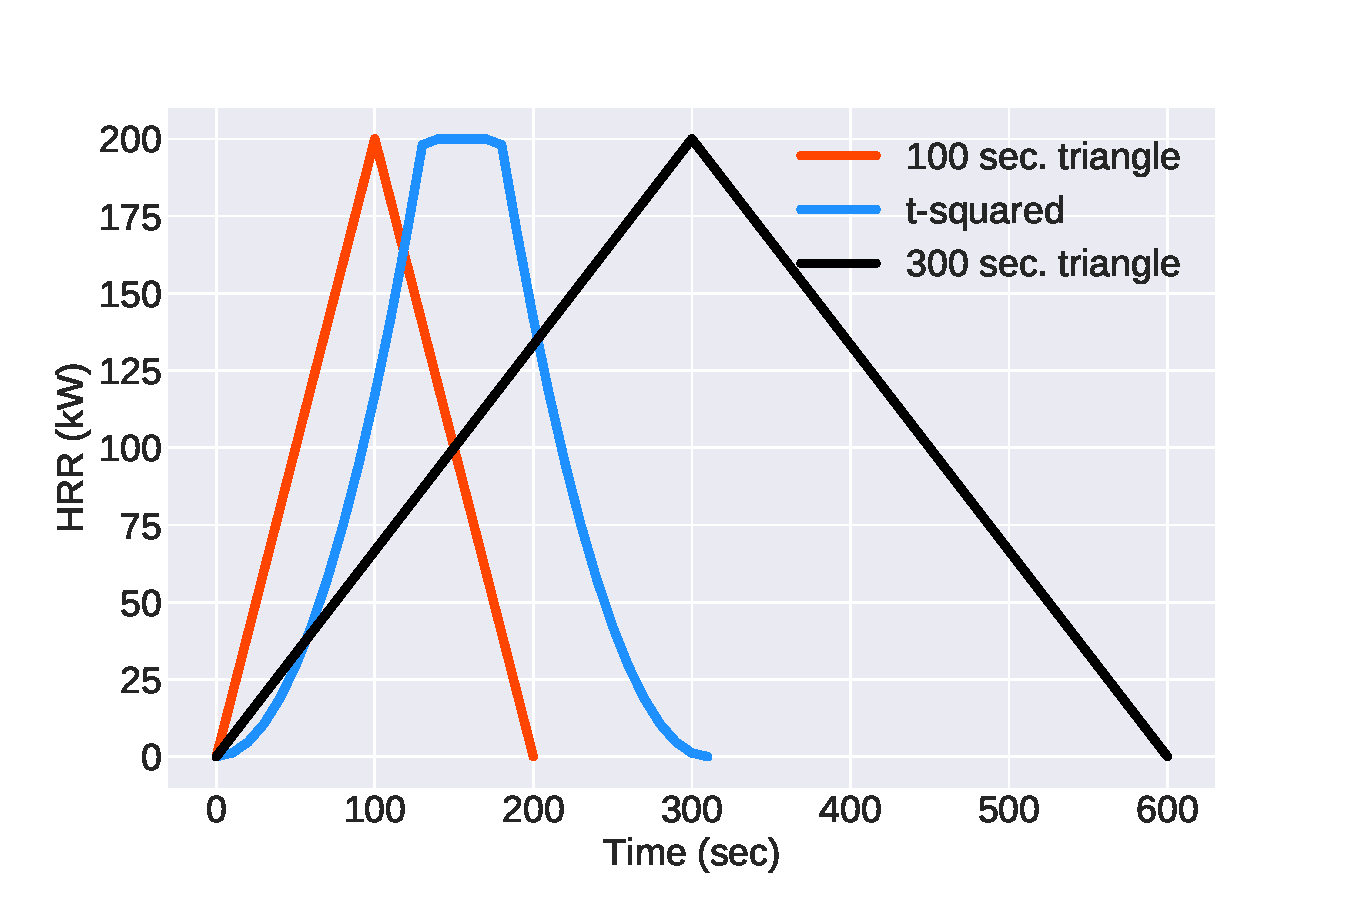
\includegraphics[width=\textwidth,keepaspectratio]{figures/training_ramps.pdf}
      \caption{Training HRR ramps}
      \label{fig:training_ramps}
  \end{subfigure}
  \begin{subfigure}[t]{.45\textwidth}
      \centering
      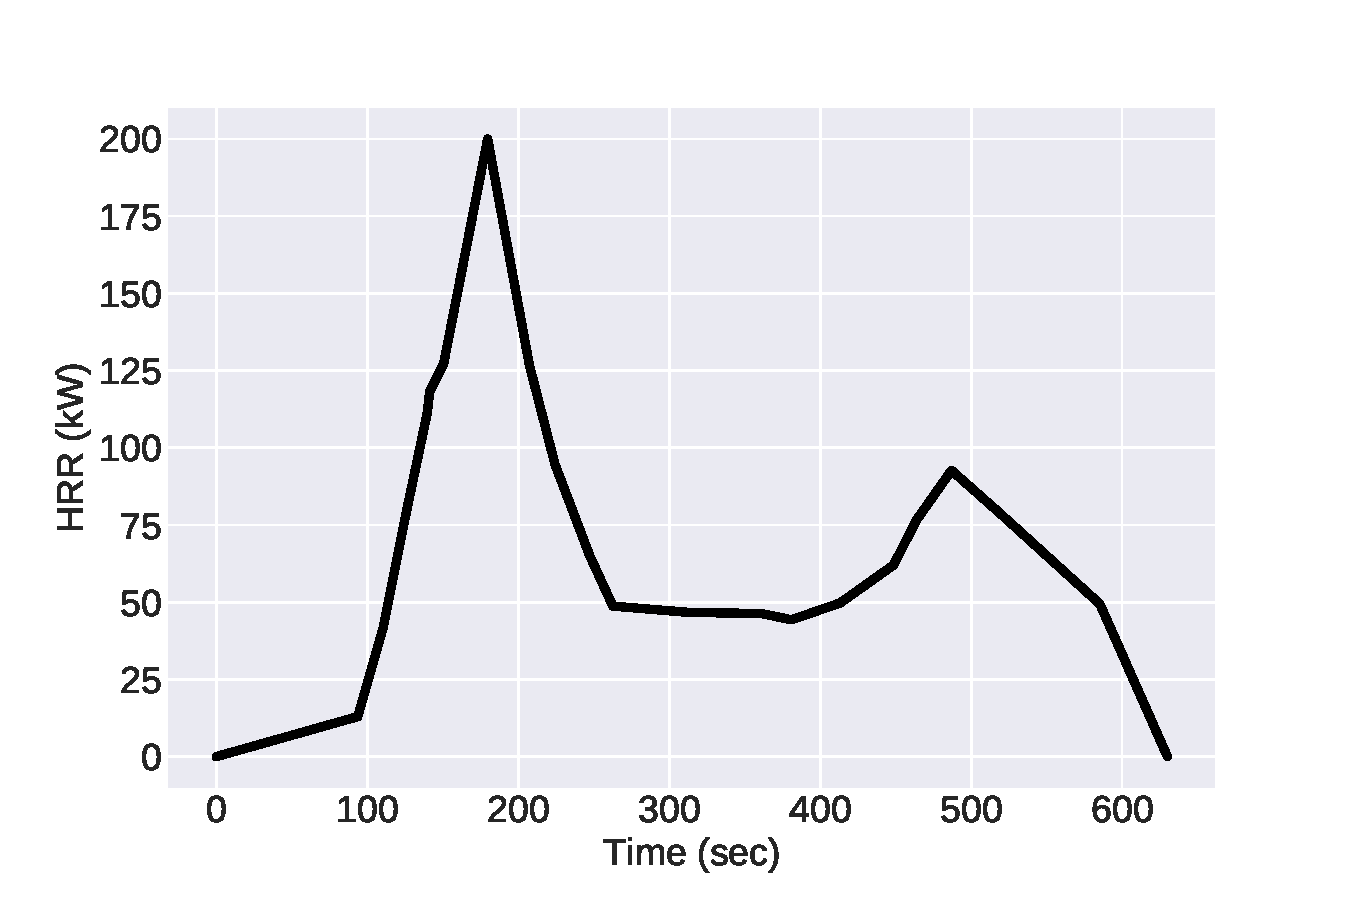
\includegraphics[width=\textwidth ,keepaspectratio]{figures/test_ramp.pdf}
      \caption{Test HRR ramp}
      \label{fig:test_ramp}
  \end{subfigure}
  \caption{\protect\ref{fig:training_ramps} shows the three HRR ramps used in the experiments that comprise the training set for the machine learning models. \protect\ref{fig:test_ramp} shows the HRR ramp used in the experiment that is used to evaluate the models. These ramps determine the setpoint for the flow rate of propane to the burner. However, the burner did not necessarily ignite immediately, so when the ramps are shown in later results, the HRR is assumed to be zero until ignition of the burner visually occurred. }
  \label{fig:hrr_ramps}
\end{figure}


\subsection{Heat flux measurements}
This section describes machine learning methods for inferring the heat release rate of a compartment fire using heat flux measurements from the directional flame thermometers (DFTs) of the aforementioned experimental setup. Modak's point source model \cite{modak1977thermal} provides a simple and intuitive relationship between a fire's heat release rate and the resulting incident radiative heat flux on a nearby target. This model assumes that the radiative energy from a fire emanates isotropically from the center of a fire such that the incident radiative heat flux on a target is described by equation \ref{eqn:point_source},

 \begin{equation}
  \label{eqn:point_source}
  q'' = \frac{\chi_R\dot{Q}cos\theta}{4\pi R^2}
\end{equation}

where $q''$ is the incident radiative heat flux at a target located at a distance $R$ from the center of the fire, $\chi_R$ is the radiative fraction of the fire, and $\theta$ is the angle between the normal to the surface of the target and the line of sight between the target and the fire. Fleury \cite{fleury2010evaluation} also evaluated six different radiation models against experimental data and found the point source model to be the most accurate. Equation \ref{eqn:point_source} suggests that if the fire and sensors are kept at fixed locations, the radiative heat release rate, $\dot{Q}_R = \chi_R\dot{Q}$ is proportional to $q''$.  This linear proportionality motivates the use of linear statistical models.  For $d$ DFTs that each took $n$ measurements throughout an experiment at times $\boldsymbol{t^{\text{DFT}}} = \begin{bmatrix}  t^{\text{DFT}}_1 & t^{\text{DFT}}_2 & \ldots & t^{\text{DFT}}_n \end{bmatrix}^T$ the linear model is 


 \begin{equation}
  \label{eqn:linear_model_expanded}
 \begin{bmatrix}
  \dot{Q}_{R}(t^{\text{DFT}}_1) \\ 
  \dot{Q}_{R}(t^{\text{DFT}}_2) \\ 
  \vdots \\
  \dot{Q}_{R}(t^{\text{DFT}}_n) \\ 
  \end{bmatrix} = \begin{bmatrix}
  q''_1(t^{\text{DFT}}_1) & q''_2(t^{\text{DFT}}_1) & \cdots & q''_d(t^{\text{DFT}}_1) \\ 
  q''_1(t^{\text{DFT}}_2) & q''_2(t^{\text{DFT}}_2) & \cdots & q''_d(t^{\text{DFT}}_2) \\ 
  \vdots & \vdots & \vdots & \vdots \\ 
  q''_1(t^{\text{DFT}}_n) & q''_2(t^{\text{DFT}}_n) & \cdots & q''_d(t^{\text{DFT}}_n) \\ 
  \end{bmatrix}
   \begin{bmatrix}
  \beta_1 \\ 
  \beta_2 \\ 
  \vdots \\
  \beta_d \\ 
  \end{bmatrix} +
    \begin{bmatrix}
  \epsilon_1 \\ 
  \epsilon_2 \\ 
  \vdots \\
  \epsilon_n \\ 
  \end{bmatrix}
\end{equation}

\noindent or written more compactly as 

 \begin{equation}
  \label{eqn:linear_model}
    \boldsymbol{\dot{Q}}_{R}  = \boldsymbol{q}'' \boldsymbol{\beta} + \boldsymbol{\epsilon}
\end{equation}

For and experiment with $n$ observations and $d$ DFTs, $\boldsymbol{\dot{Q}}_{R} \in  \mathbb{R}^n$ is a vector of radiative HRR values, $\boldsymbol{q}'' \in \mathbb{R}^{n\text{x}m}$ is a matrix of heat flux measurements, $\boldsymbol{\beta} \in \mathbb{R}^n$ is a vector of regression slopes, and $\boldsymbol{\epsilon} \in \mathbb{R}^n$ is vector of random errors. Note that the model assumes that $\chi_R$ is constant throughout an experiment; it is not necessarily constant across different experiments if different fuels are used. If only one DFT were used, the point source model would suggest that $\beta = \frac{4 \pi R^2}{ cos \theta}$. However, this is not true for the multivariate case, and as a result, the coefficients of $\boldsymbol{\beta}$ are instead learned from the experimental data in the training set.

In addition to the theoretical explanation from Modak's point source model, the scatterplots shown in Figure \ref{fig:dft_scatterplot} show the linear relationship between the radiative heat release rate, $\boldsymbol{\dot{Q}}_{R}$ and $\boldsymbol{q}''$ from the training set experiments. 

\begin{figure}[htbp]
  \centering
  \begin{subfigure}[t]{.45\textwidth}
      \centering
      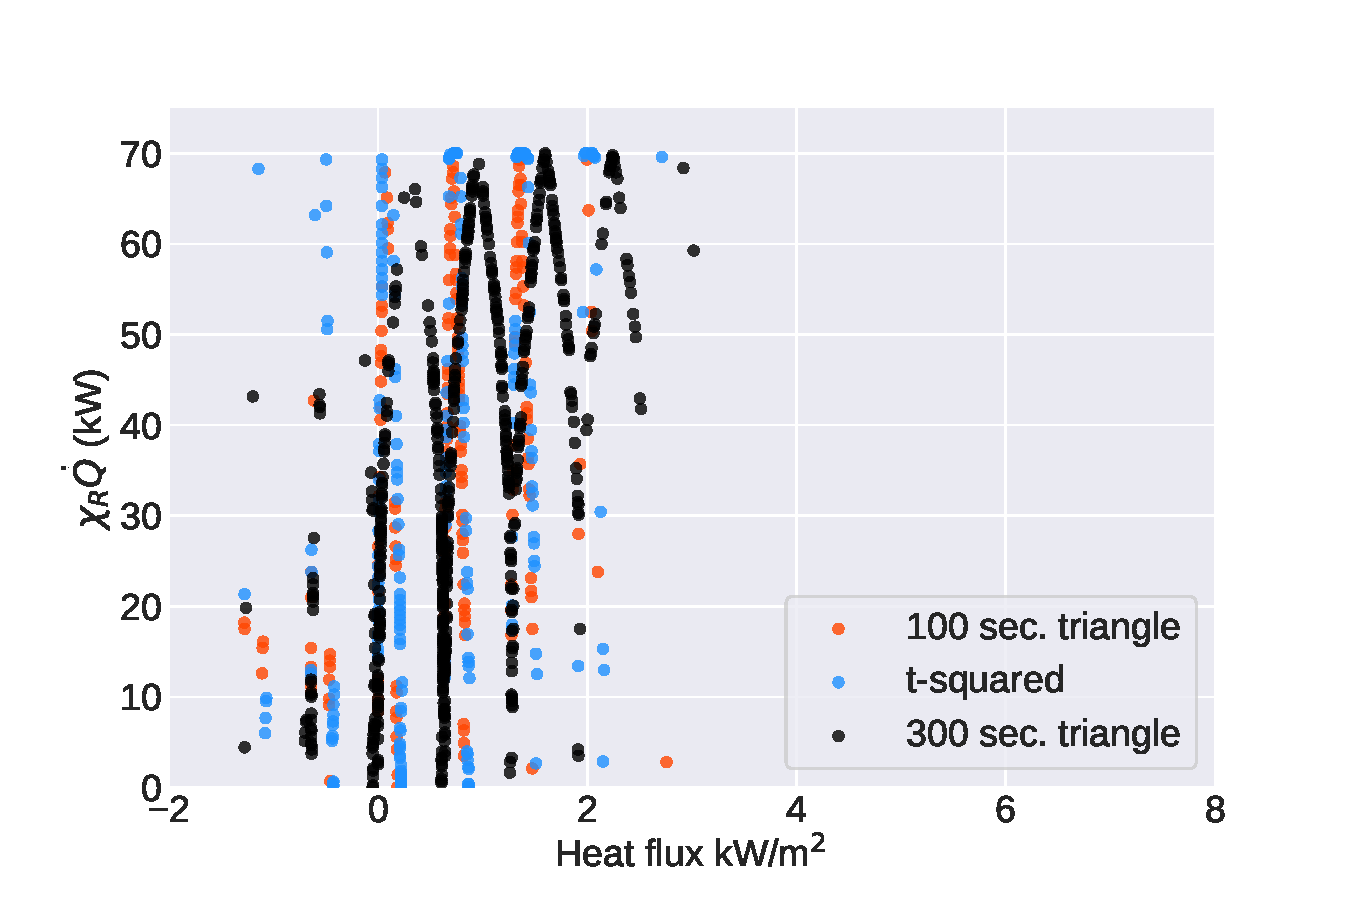
\includegraphics[width=\textwidth,keepaspectratio]{figures/weak_dft_scatter.pdf}
      \caption{Weak correlation}
      \label{fig:weak_scatter}
  \end{subfigure}
  \begin{subfigure}[t]{.45\textwidth}
      \centering
      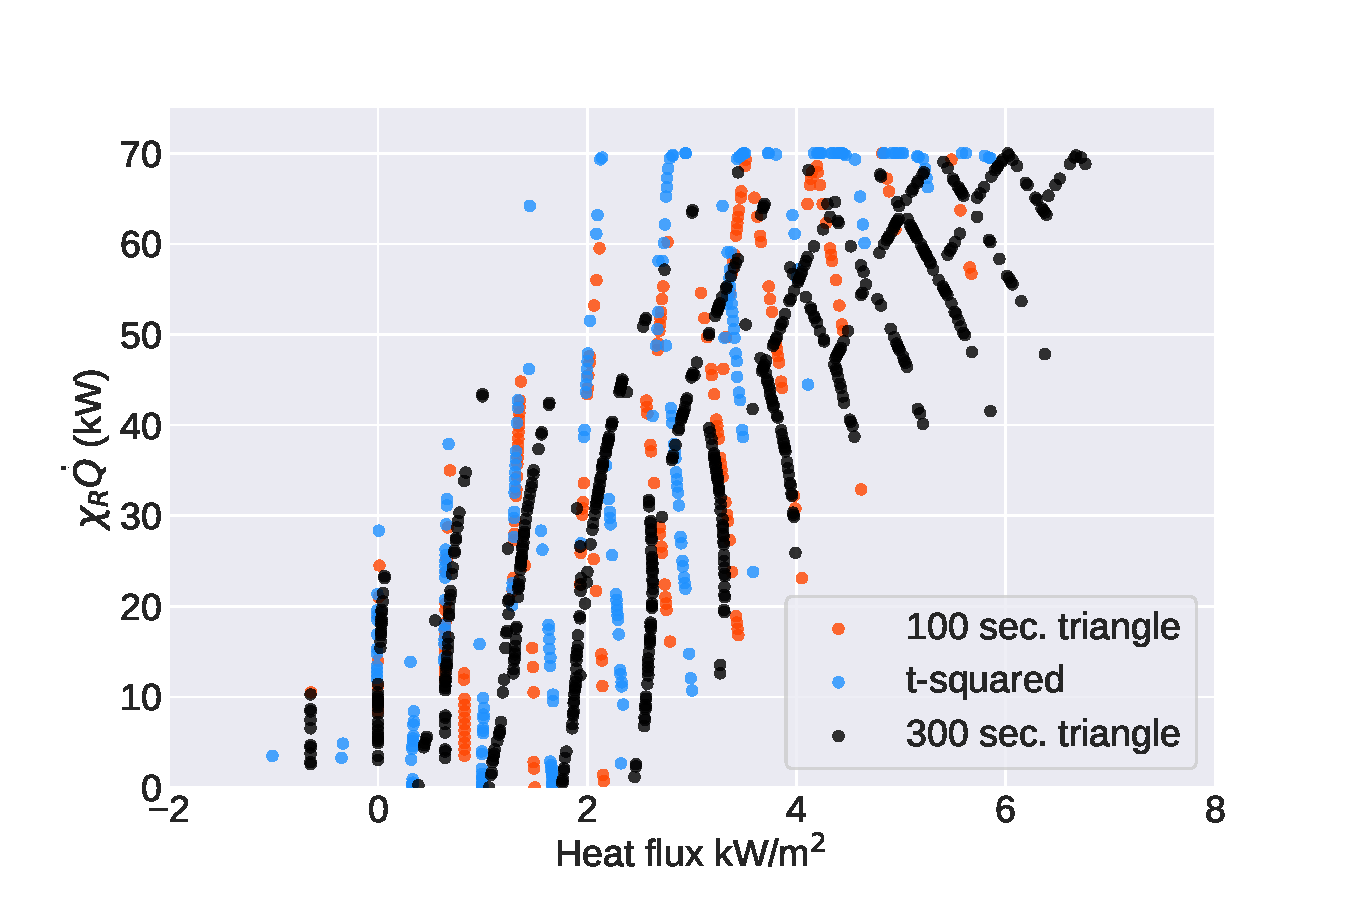
\includegraphics[width=\textwidth ,keepaspectratio]{figures/moderate_dft_scatter.pdf}
      \caption{Moderate correlation}
      \label{fig:moderate_scatter}
  \end{subfigure}
   \begin{subfigure}[t]{.45\textwidth}
      \centering
      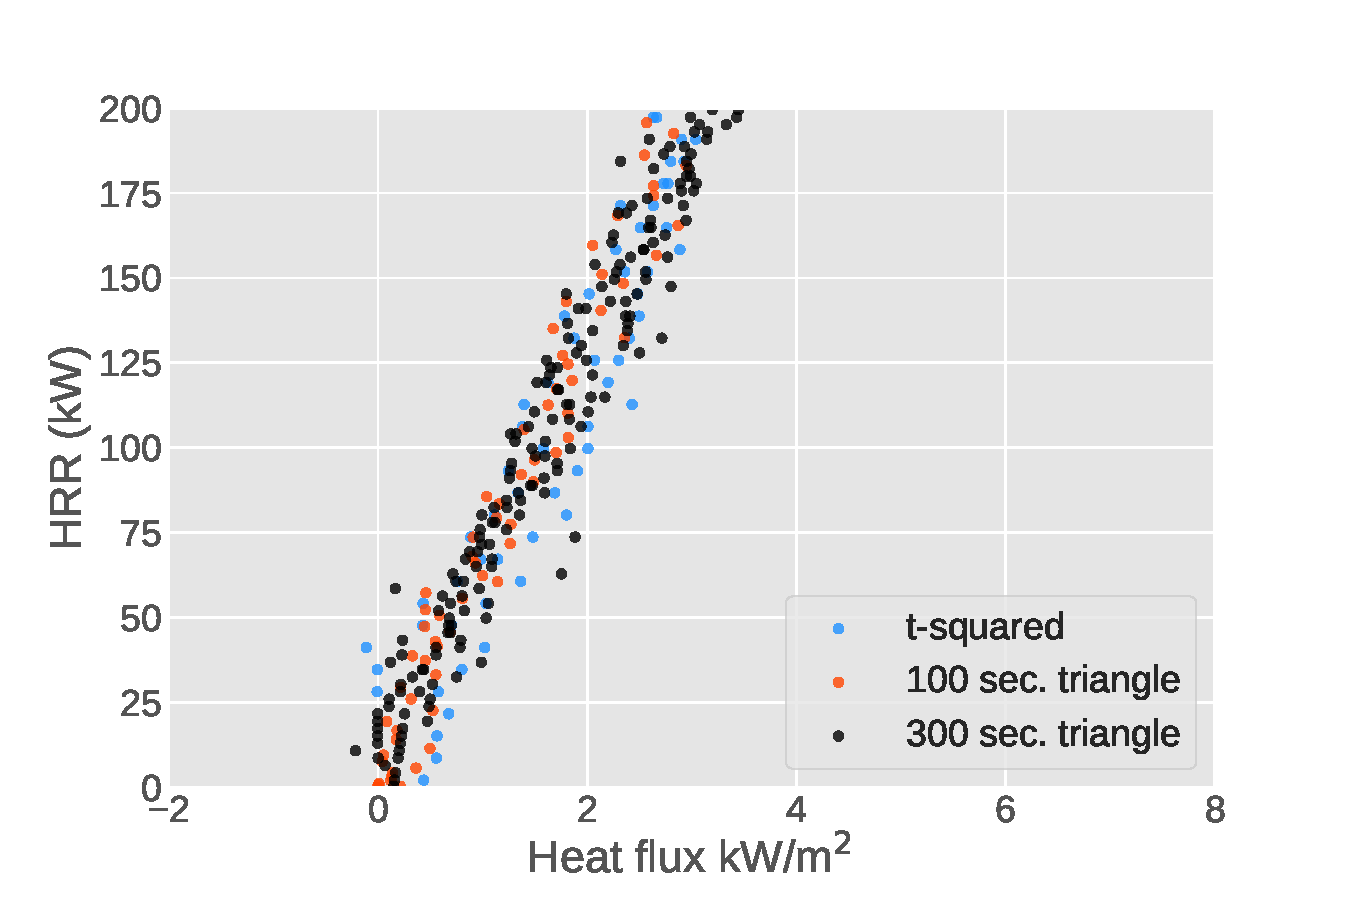
\includegraphics[width=\textwidth ,keepaspectratio]{figures/strong_dft_scatter.pdf}
      \caption{Strong correlation}
      \label{fig:strong_scatter}
  \end{subfigure}
  \caption{Scatterplots of the radiative heat release rate vs. measured heat flux for three different DFTs. These examples demonstrate the variation in the strength of correlations across DFTs. The measurement at each second of the training set experiments is shown.} 
  \label{fig:dft_scatterplot}
\end{figure}

The examples shown in Figure \ref{fig:dft_scatterplot} demonstrate how the strength of the correlation between the radiative HRR and measured heat flux varies significantly across the different DFTs. This finding raises several questions regarding the design of the model. First, should all the DFTs be included in the model? If not, which ones should be excluded and why? It may seem that the best set of sensors to include in the model is the one that includes only the DFTs whose measured heat flux is the most correlated with the radiative heat release rate. However, this is not necessarily true because multiple DFTs with strong correlations can provide redundant information. Also, the presence of multicollinearity can reduce the predictive accuracy of a linear regression model. This refers to the fact that the input features are correlated with each other; the measured heat fluxes will generally increase or decrease in parallel. 

To circumvent these issues, a lasso regression is employed using the Scikit-learn \cite{pedregosa2011scikit} package in Python . This technique is a modified linear regression that performs feature selection in addition to estimating values of $\boldsymbol{\beta}$. These values are estimated according to equation \ref{eqn:lasso}:

 \begin{equation}
  \label{eqn:lasso}
  \boldsymbol{\hat\beta}_{lasso} = \argmin_{\boldsymbol{\beta}}\Bigg\{ \underbrace{\big[\boldsymbol{\dot{Q}}_{R} - \boldsymbol{q}'' \boldsymbol{\beta}\big]^T\big[ \boldsymbol{\dot{Q}}_{R} - \boldsymbol{q}'' \boldsymbol{\beta}\big]}_{\text{I}} + \underbrace{\lambda||\boldsymbol{\beta}||_1}_{II}   \Bigg\}
\end{equation}

\noindent where $||\boldsymbol{\beta}||_1 = \sum_i{|\beta_i|}$ is the L1 norm of $\boldsymbol{\beta}$ and $\lambda$ is a hyperparameter that is learned from the data through 5-fold cross validation. This refers to the process of randomly splitting the training set into five different groups. For a given $\lambda$, lasso regression is fit using four of the five groups, and the model is scored based on its ability to make predictions on the excluded group. Specifically, the score is the coefficient of determination ($R^2$). This process is conducted five times so that each group is excluded once. The score for a given $\lambda$ is evaluated by averaging the scores across the five iterations of the cross validation and the $\lambda$ providing the best score is selected for the model. 

Note that term I is simply the sum of the squared residuals, meaning that if term II is zero, the process is identical to a ordinary least squares linear regression. The inclusion of term II, also known as L1 regularization, serves two purposes. First, it helps prevent overfitting as term II can be viewed as a penalty for increased model complexity. Second, it performs feature selection because the L1 regularization has a tendency to set values in $\boldsymbol{\beta}$ to zero, thereby removing the corresponding features from the model. It should be noted that the use of the $l^2$ norm (known as ridge regression, which is used later in this paper) is another common technique to combat overfitting; however, unlike lasso regression, ridge regression does not also perform feature selection. 

Figure \ref{fig:lasso_graphic} is a graphical illustration of the lasso regression framework. For a simple two variable regression model, $\boldsymbol{\dot{Q}}_{R} = q''_1\beta_1 + q''_2\beta_2$, the sum of the squared residuals, $[\boldsymbol{\dot{Q}}_{R} - \boldsymbol{q}'' \boldsymbol{\beta}\big]^T\big[\chi_R \boldsymbol{\dot{Q}}_{R} - \boldsymbol{q}'' \boldsymbol{\beta}]$, is the colored contour plot, whose minimum is indicated by the ``x" marker. If one were to perform an ordinary linear regression, the $\beta_1$ and $\beta_2$ that provide this optimum would be chosen. The lasso regression framework penalizes sets of $\boldsymbol{\beta}$ that are further away from the origin by a L1 or ''Manhattan" distance measure. A diamond comprises the set of locations that are a constant L1 distance from the origin, just as a circle would comprise the set of points that are a constant L2 distance from the origin. Intuitively, one can imagine a optimization problem in which the goal is to minimize the sum of the squared residuals while remaining within a specified L1 distance from the origin. The diamond shape of constant L1 contours gives the optimal $\beta$ a tendency to contain zeros. The black diamond marker indicates this optimum, which sets $\beta_2$ to zero, thereby removing $q''_2$ from the model. 

\begin{figure}[htb] \centering
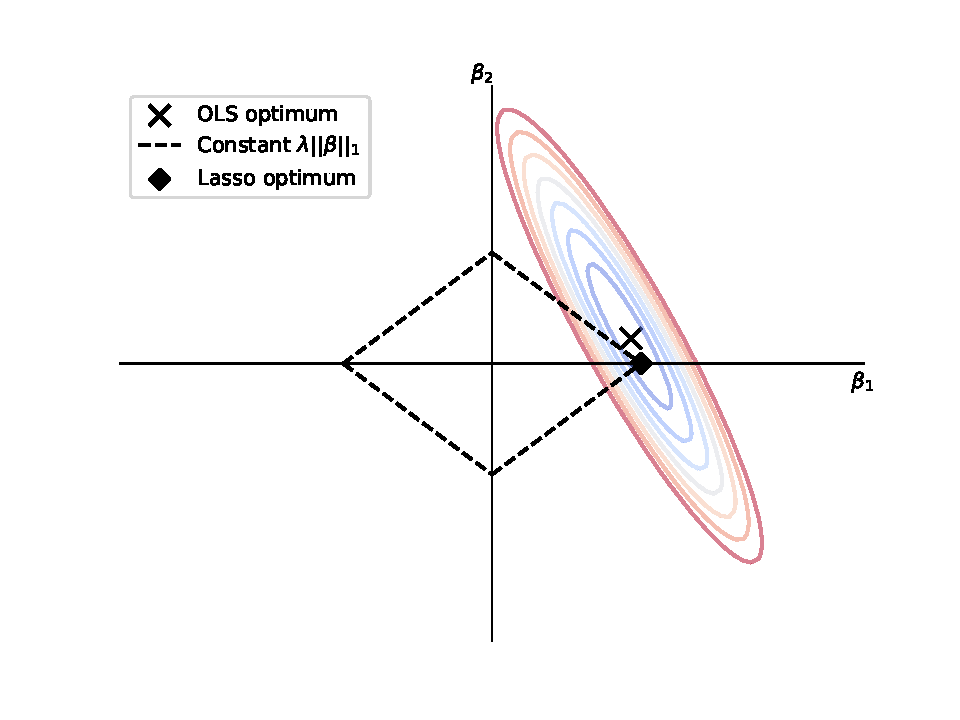
\includegraphics[width=.75\textwidth]{./figures/lasso_graphic.pdf}
\caption{A graphical illustration of the lasso regression framework. The colored contour plot shows the sum of the squared residual function, $[ \boldsymbol{\dot{Q}}_{R} - \boldsymbol{q}'' \boldsymbol{\beta}\big]^T\big[ \boldsymbol{\dot{Q}}_{R} - \boldsymbol{q}'' \boldsymbol{\beta}]$. The ``x" marker indicates the minimum of this function, which would determine $\boldsymbol{\beta}$ in an ordinary linear regression framework. However, in a lasso regression framework, there is a penalty for sets of coefficients that are further away from the origin according to the L1 distance. The dashed diamond comprises a set of points that are a constant L1 distance from the origin, and the black diamond marker indicates the solution to equation \protect\ref{eqn:lasso}.}
\label{fig:lasso_graphic}
\end{figure}

Figure \ref{fig:dft_regressions} shows a comparison of the predicted HRR curves produced by an ordinary linear regression (\ref{fig:linreg_rad}) and a lasso regression (\ref{fig:lasso_rad}).

\begin{figure}[htbp]
  \centering
  \begin{subfigure}[t]{.45\textwidth}
      \centering
      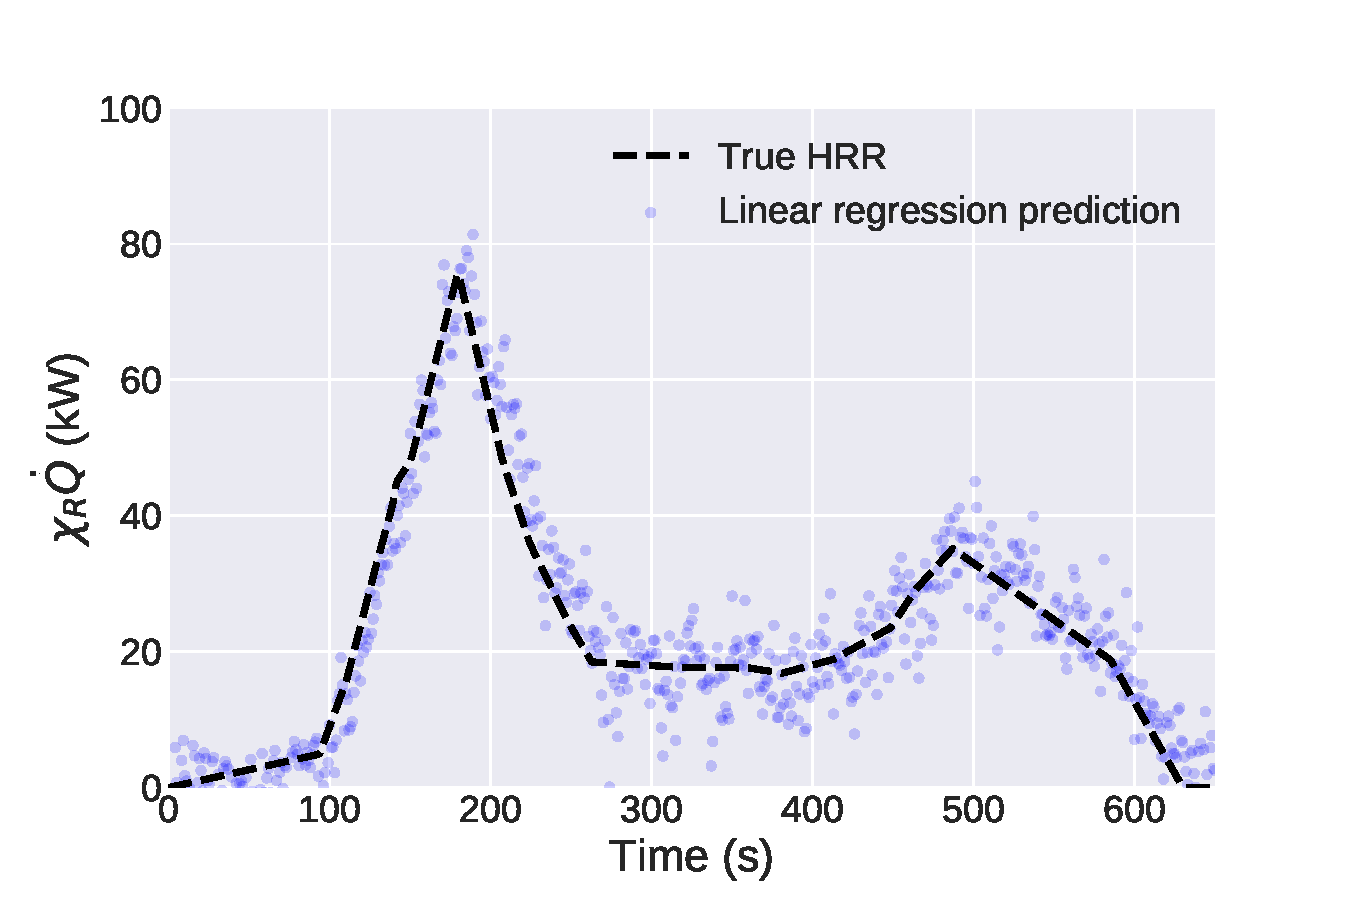
\includegraphics[width=\textwidth,keepaspectratio]{figures/linreg_rad.pdf}
      \caption{Linear regression (33 sensors)}
      \label{fig:linreg_rad}
  \end{subfigure}
  \begin{subfigure}[t]{.45\textwidth}
      \centering
      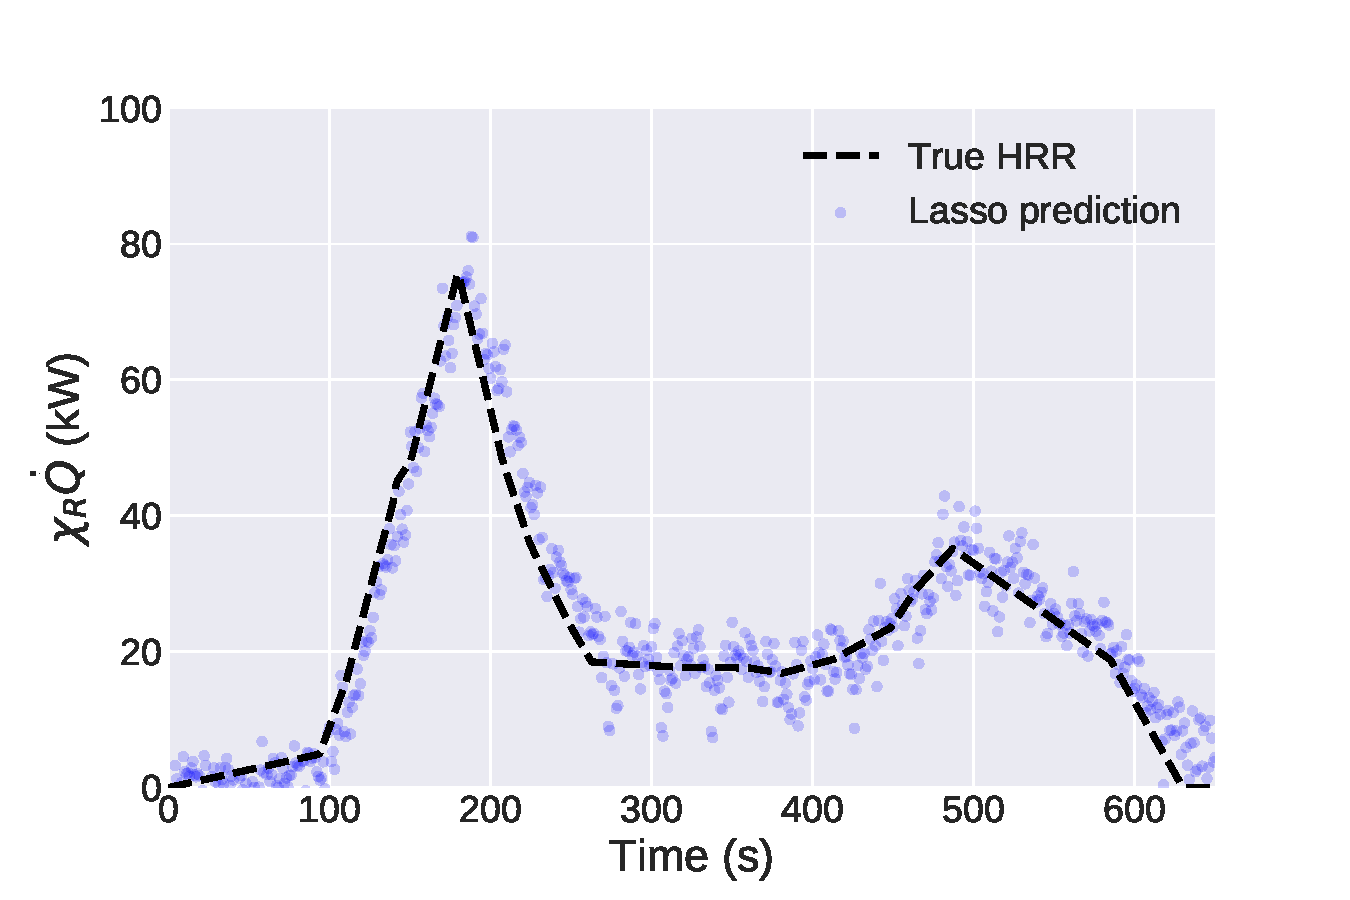
\includegraphics[width=\textwidth ,keepaspectratio]{figures/lasso_rad.pdf}
      \caption{Lasso regression (13 sensors)}
      \label{fig:lasso_rad}
  \end{subfigure}
  \caption{A comparison of the predicted HRR curves between an ordinary linear regression and a lasso regression. The mean absolute error add_value between the two approaches is similar, but the lasso regression is preferred because it uses only 13 DFTs as opposed to the linear regression which uses all 33 DFTs. } 
  \label{fig:dft_regressions}
\end{figure}

The lasso regression excludes 20 of the 33 DFTs from the model. Figure \ref{fig:lasso_dfts} shows locations of the DFTs included in the model and their corresponding regression coefficients ($\beta_i$).

\begin{figure}[htb] \centering
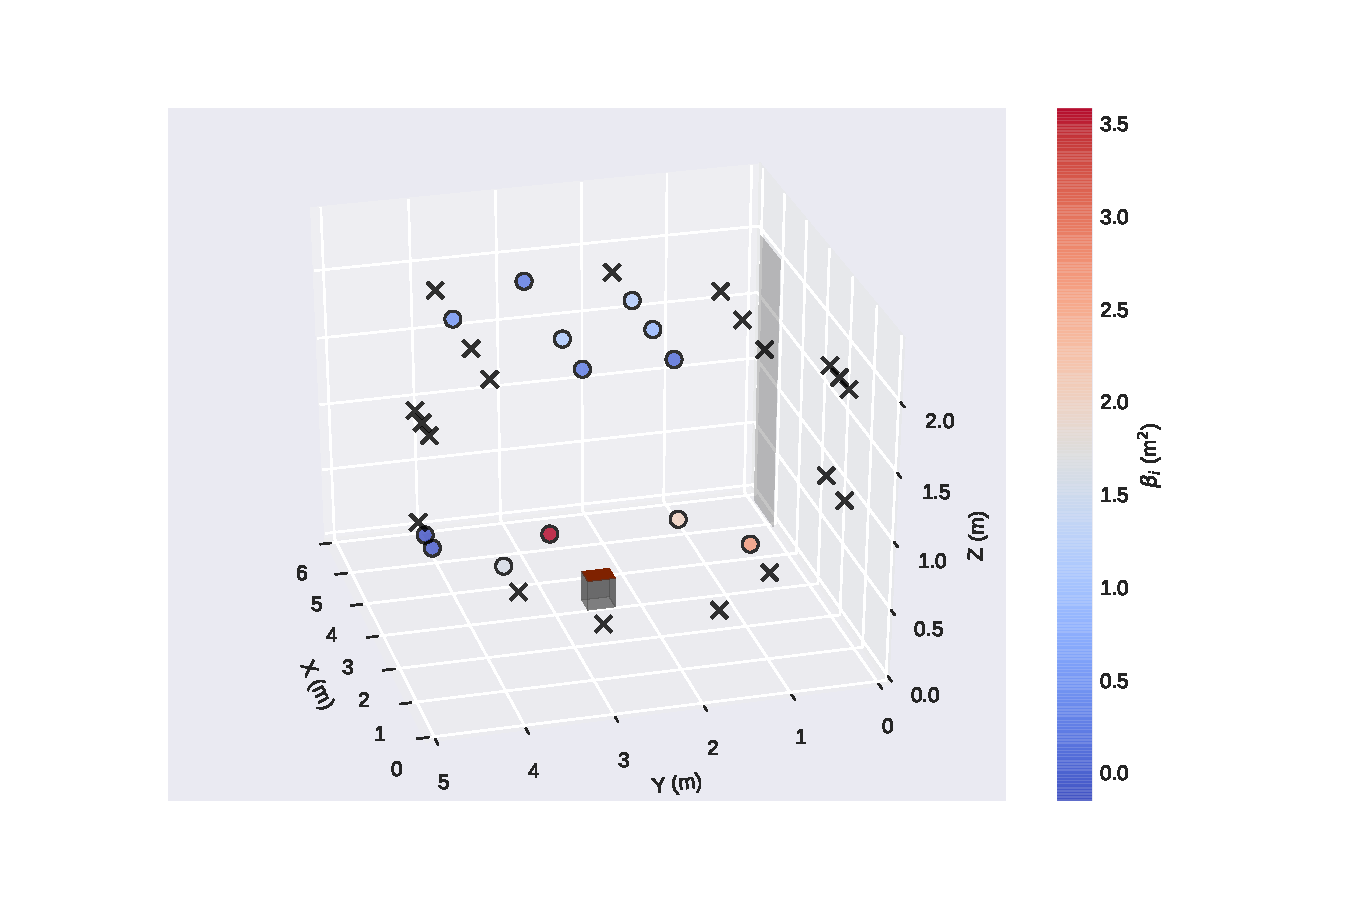
\includegraphics[width=.75\textwidth]{./figures/lasso_dfts.pdf}
\caption{A schematic of the of the burn structure and the DFTs with all DFT locations shown. The ``x" markers indicate DFTs that are excluded by the lasso regression. The circles indicate DFTs included in the lasso regression, and their color indicates the corresponding regression coefficient. The locations of the open door and the burner are also shown. Note the dimensions of $\beta_i$ are heat release rate per heat flux and the units are $m^2$.}
\label{fig:lasso_dfts}
\end{figure}

The lasso regression most greatly weights the heat fluxes of the low DFTs surrounding the burner in its predictions. This is not surprising given that these sensors are the closest to the burner, which likely means that their measurements are the most sensitive to the heat release rate. Also, because these sensors are low to the ground, they likely do not experience significant convective heating, which could introduce error. During the experiments, the authors noticed that the flame has a tendency to lean at different angles in the y-z plane, which could explain the relatively large weight placed into the DFT that lies in the negative-y direction from the burner. The inclusion of the DFTs near the ceiling is possibly due to the fact that the virtual radiation source of the fire grows with increasing HRR.

It should be noted that until this point, the model does not include any transient information, meaning that the lasso regression predicts $\boldsymbol{\dot{Q}}_{R}$ at an instant in time based on the measured heat fluxes at that same instant. It does not consider the history of heat fluxes nor the history of $\boldsymbol{\dot{Q}}_{R}$. As a result, the predictions significantly fluctuate over short timescales, but it is believed that the underlying HRR curve does not. This motivates the use of a temporal smoother to improve the predicted radiative HRR curve. Although there are many types of smoothers that could be used, the authors opted to use Gaussian process regression (also known as kriging) because it is a integral concept of later results in this paper. 

It is reasonable to expect that the lasso predictions are actually noisy draws centered around an underlying ``smoother" function. Mathematically, this can be written as

 \begin{equation}
  \label{eqn:gaussian_process_model}
  \dot{Q}_{R}^{\text{lasso}}(t) = \dot{Q}_{R}^{\text{GP}}(t) + \epsilon(t)
\end{equation}

where $\dot{Q}_{R}^{\text{lasso}}(t)$ is the lasso prediction at time $t$. The error, $\epsilon(t) \sim N(0,\sigma^2)$, is normally distributed with variance $\sigma^2$, and finally $\dot{Q}_{R}^{\text{GP}}(t)$ is the underlying function that Gaussian proccess regression (GPR) attempts to learn. A Gaussian process is a stochastic process in which any finite collection of random variables has a joint multivariate normal distribution \cite{lee2017deep}. Loosely speaking, a Gaussian process can be viewed as a probability distribution of functions, which may seem abstract to readers unfamiliar with this type of statistical modeling, especially because these functions do not have a specified form (linear, polynomial, etc). If one imagines a distribution of functions, then a random sample of $N$ functions could be collected from the distribution. Each of these functions could then be evaluated at some arbitrary time, $t_1$, producing a set of $N$ scalar values. If the distribution of functions meets the definition of a Gaussian process, then this sample of scalar values will reveal a univariate normal distribution (assuming $N$ is large enough to capture the population distribution). Similarly, these functions could be evaluated at two different times, $t_1, t_2$, and the vector of function evaluations would have a bivariate normal distribution. Any vector of $n$ function evaluations, $f(\boldsymbol{t})$, will follow a multivariate normal distribution, whose form is shown in equation \ref{eqn:multivariate_gaussian}.

 \begin{equation}
  \label{eqn:multivariate_gaussian}
  p\bigg(f(\boldsymbol{t}) \bigg) = \mathcal{N}\Big(\boldsymbol{\mu}, \boldsymbol{\Sigma} \Big) = 
  (2\pi)^{-\frac{n}{2}}\text{det}\big[\boldsymbol{\Sigma}\big]^{-\frac{1}{2}}\text{exp}\bigg(-\frac{1}{2}\big[f(\boldsymbol{t}) - \boldsymbol{\mu}\big]^T \boldsymbol{\Sigma}^{-1}\big[f(\boldsymbol{t}) - \boldsymbol{\mu}\big] \bigg)
\end{equation}

Just as a univariate normal distribution is uniquely characterized by a scalar mean and a scalar variance, a multivariate normal distribution is uniquely characterized by a mean vector $\boldsymbol{\mu}$ and a symmetirc positive semi-definite covariance matrix, $\boldsymbol{\Sigma}$, whose entries are described by equation \ref{eqn:covariance_matrix}.

 \begin{equation}
  \label{eqn:covariance_matrix}
  \Sigma_{i,j} = E\bigg([x_i- \mu_i][x_j - \mu_j] \bigg)
\end{equation}

Going back to the thought experiment of drawing functions from a distribution, one can imagine drawing a random sample of $N$ functions and evaluating each function at the same two points, $t_i$ and $t_i + \Delta t$. If $\Delta t$ is small, then one would expect that the function evaluations at $t_i$ and $t_i + \Delta t$ would be similar (correlated), depending on how smooth the drawn functions are. In the limiting case, when $\Delta t = 0$, the function evaluations will be exactly the same (perfectly correlated) if the functions are continuous. Conversely, if $\Delta t$ is large, then the two quantities will generally be uncorrelated. This motivates the use of a function to quantify the covariance between function evaluations at different points based on the size of the interval between the two points. Specifically, the authors use a squared exponential kernel function, shown in equation \ref{eqn:squared_exponential}, 


 \begin{equation}
  \label{eqn:squared_exponential}
    K(t_i, t_j) = \tau^2exp\bigg(-\frac{(t_i-t_j)^2}{2b^2}\bigg)
\end{equation}

\noindent where $\tau^2$ is a hyperparameter that describes the magnitude of the function draws, and $b$, known as the bandwidth, relates to the time scale over which function evaluations are correlated. Intuitively, $b$ defines how smooth the function draws will be, with a larger bandwidth giving smoother functions. As previously noted, a mean vector and a covariance function uniquely characterize a multivariate normal distribution. Similarly, a mean function, $m$, and a kernel function, $K$, uniquely characterize a Gaussian process. For any vector of times $\boldsymbol{t} = \begin{bmatrix}  t_1 & t_2, & \ldots & t_n \end{bmatrix}^T$, if $f(t) \sim \mathcal{GP}(m,K)$, then $f(\boldsymbol{t}) \sim \mathcal{N}\Big(m(\boldsymbol{t}), \boldsymbol{\Sigma}\Big)$, where $\boldsymbol{\Sigma} =  K(\boldsymbol{t},\boldsymbol{t})$, i.e. $\Sigma_{i,j} = K(t_i, t_j)$. 

The concept of Gaussian processes allows for a flexible Bayesian regression framework. The general idea is that the uncertainty of an underlying function is described as a Gaussian process. A prior distribution is first constructed, describing a relatively wide variety of functions. However, many of these functions are unlikely given the degree of mismatch with the observed data as well as the assumptions made in equation \ref{eqn:gaussian_process_model}. Using Bayes' law, a posterior distribution for  $\dot{Q}_{R}^{\text{GP}}(t)$ is obtained. Although this distribution is not the distribution for the true radiative HRR, $\dot{Q}_{R}(t)$, it produces significantly more accurate estimations of $\dot{Q}_{R}(t)$ than the lasso framework does in isolation. 


The first step in the methodology is to define a prior for $\dot{Q}_{R}^{\text{GP}}(t)$. A common choice for a prior is a Gaussian process with mean zero \cite{rasmussen2003gaussian}, i.e. $\dot{Q}_{R}^{\text{GP}}(t) \sim \mathcal{GP}(0, K)$ The astute reader may notice that the prior is not yet fully defined because the hyperparameters, $\tau^2$ and $b$, have not been specified in the kernel function (equation \ref{eqn:squared_exponential}). One approach would be to specify priors for these parameters, resulting in a fully Bayesian Gaussian process regression model. For simplicity, the authors instead opt to determine these parameters by maximizing the marginal likelihood, which is again a common practice \cite{rasmussen2003gaussian}. The idea behind this approach is to choose the $\tau^2$ and $b$ that generate the prior distribution that is most likely to produce the observed data given the assumptions of equation \ref{eqn:gaussian_process_model}. Recall that lasso predictions are computed for every time in the vector $\boldsymbol{t^{\text{DFT}}} = \begin{bmatrix}  t^{\text{DFT}}_1 & t^{\text{DFT}}_2 & \ldots & t^{\text{DFT}}_n \end{bmatrix}^T$. Given the Gaussian process prior, the distribution of function evaluations for these times is multivariate normal. Specifically,  $\dot{Q}_{R}^{\text{GP}}(\boldsymbol{t^{\text{DFT}}}) \sim \mathcal{N}\Big(\boldsymbol{0}, \  K( \boldsymbol{t^{\text{DFT}}}, \boldsymbol{t^{\text{DFT}}}, \tau^2, b) \Big)$ Note the explicit indication of the fact that the covariance matrix returned by the kernel function depends on the hyperparameters $\tau^2$ and $b$. Recall that the lasso predictions, $\dot{Q}_{R}^{\text{lasso}}(\boldsymbol{t^{\text{DFT}}})$,  are assumed to be $\dot{Q}_{R}^{\text{GP}}(\boldsymbol{t^{\text{DFT}}})$ plus a vector of random Gaussian noise, $\boldsymbol{\epsilon} \sim \mathcal{N}(\boldsymbol{0}, \sigma^2\boldsymbol{I})$, where $\boldsymbol{I}$ is the identity matrix. The variance $\sigma^2$ can be estimated by examining the scatter of the lasso predictions around the true HRR for an experiment in the training set according to equation \ref{eqn:sigma_estimate}: 

 \begin{equation}
  \label{eqn:sigma_estimate}
    \sigma^2 \approx \sum_{i=1}^{N_{exp}}\frac{\Big[\dot{Q}_{R}^{\text{lasso}}(t^{\text{DFT}}_i) - \dot{Q}_{R}(t_i^{\text{DFT}})\Big]^2}{N_{exp}-1} 
\end{equation}

\noindent where $N_{exp}$ is the length of $\boldsymbol{t}^{\text{DFT}}$ for the experiment used for this estimation. The authors used the 100 second triangle fire for this calculation, but the results are similar regardless of which experiment is chosen. Technically $\sigma^2$ is the variance of the lasso predictions around $\dot{Q}_{R}^{\text{GP}}(t)$ rather than the true radiative HRR, $\dot{Q}_{R}(t_i^{\text{DFT}})$, but equation \ref{eqn:sigma_estimate} is a convenient approximation. Also, recall that $\dot{Q}_{R}(\boldsymbol{t}^{\text{DFT}})$ is known for the experiments in the training set because they are viewed as calibration experiments.


 Because $\dot{Q}_{R}^{\text{lasso}}(\boldsymbol{t^{\text{DFT}}})$ is the sum of two (multivariate) normally distributed random variables, it is also normally distributed; its mean vector is the sum of the two mean vectors and its covariance matrix is the sum of the two covariance matrices, i.e. $\dot{Q}_{R}^{\text{lasso}}(\boldsymbol{t^{\text{DFT}}}) \sim \mathcal{N}\Big(\boldsymbol{0}, \ K( \boldsymbol{t^{\text{DFT}}}, \boldsymbol{t^{\text{DFT}}}, \tau^2, b) + \sigma^2\boldsymbol{I} \Big)$. Therefore the probability density function (PDF), $p\Big(\dot{Q}_{R}^{\text{lasso}}(\boldsymbol{t^{\text{DFT}}}), \tau, b \Big)$, follows the form of equation \ref{eqn:multivariate_gaussian}. Plugging in the vector of observed lasso predictions for and individual experiment gives a scalar probability density, or \textit{likelihood}, that depends on $\tau^2$ and $b$. Using a Nelder-Mead optimization algorithm \cite{nelder1965simplex} implemented in the python package Scipy \cite{jones2001scipy}, the optimal hyperparameters, $\tau^2_{\text{opt}}$ and $b_{\text{opt}}$ are chosen according to equation \ref{eqn:max_likelihood}. The initial guess for $b$ is 10 seconds and the initial guess for $\tau^2$ is 5,000 kW$^2$. 

\begin{equation}
  \label{eqn:max_likelihood}
  \tau^2_{\text{opt}}, \ b_{\text{opt}} = 
  \argmax_{\tau^2, b} \Bigg\{log\bigg[ p\Big(\dot{Q}_{R}^{\text{lasso}}(\boldsymbol{t^{\text{DFT}}}), \tau, b \Big)\bigg] \Bigg\}
\end{equation}

Once the hyperparameters are optimized, the prior is fully specified. Figure \ref{fig:gp_prior} shows five functions drawn from the Gaussian process (sampled every second). The next step is to update the prior given the observed data using Bayes' law. Specifically, the objective is to compute the probability distribution of $\dot{Q}_{R}^{\text{GP}}(\boldsymbol{t^{*}})$ evaluated at an arbitrary vector of times, $\boldsymbol{t}^* = \begin{bmatrix}  t^*_1 & t^*_2 & \ldots & t^*_p \end{bmatrix}^T$ given the prior and the observed lasso predictions evaluated at $\boldsymbol{t^{\text{DFT}}}$. Given that $\dot{Q}_{R}^{\text{GP}}(t) \sim \mathcal{GP}(0,K_{\text{opt}})$, where $K_{\text{opt}}$ indicates the kernel function with optimized hyperparameters, the function evaluations for any vector of times produces a multivariate normal distribution. If $\boldsymbol{t^{\text{DFT}}}$ and $\boldsymbol{t^{*}}$ are concatenated into a single vector, $\begin{bmatrix} \boldsymbol{t^{\text{DFT}}} & \boldsymbol{t^{*}} \end{bmatrix}^T \in \mathbb{R}^{n+p}$, then the corresponding joint distribution of function evaluations can be written as 

\begin{equation}
  \label{eqn:joint_GP}
  \begin{bmatrix}
  \dot{Q}_{R}^{\text{GP}}(\boldsymbol{t}^{\text{DFT}}) \\
  \dot{Q}_{R}^{\text{GP}}(\boldsymbol{t}^*)
  \end{bmatrix} \sim 
  \mathcal{N} \Bigg(\boldsymbol{0}, 
  \begin{bmatrix}
 K_{\text{opt}}(\boldsymbol{t}^{\text{DFT}}, \boldsymbol{t}^{\text{DFT}}) & K_{\text{opt}}(\boldsymbol{t}^{\text{DFT}}, \boldsymbol{t}^*) \\ 
   K_{\text{opt}}(\boldsymbol{t}^*, \boldsymbol{t}^{\text{DFT}}) &  K_{\text{opt}}(\boldsymbol{t}^*, \boldsymbol{t}^*) 
  \end{bmatrix}
  \Bigg)
\end{equation}

Note that the $n$+$p$ by $n$+$p$ covariance matrix is shown as a block matrix comprised of four smaller matrices. As previously stated, equation \ref{eqn:gaussian_process_model} indicates that   $\dot{Q}_{R}^{\text{lasso}}(\boldsymbol{t^{\text{DFT}}}) \sim \mathcal{N}\Big(\boldsymbol{0}, \ K_{\text{opt}}( \boldsymbol{t^{\text{DFT}}}, \boldsymbol{t^{\text{DFT}}}) + \sigma^2\boldsymbol{I} \Big)$, which allows equation \ref{eqn:joint_GP} to be expressed in terms of the lasso predictions, $\dot{Q}_{R}^{\text{lasso}}(\boldsymbol{t^{\text{DFT}}})$, shown below:


\begin{equation}
  \label{eqn:joint_GP_lasso}
  \begin{bmatrix}
  \dot{Q}_{R}^{\text{lasso}}(\boldsymbol{t}^{\text{DFT}}) \\
  \dot{Q}_{R}^{\text{GP}}(\boldsymbol{t}^*)
  \end{bmatrix} \sim 
  \mathcal{N} \Bigg(\boldsymbol{0}, 
  \begin{bmatrix}
 K_{\text{opt}}(\boldsymbol{t}^{\text{DFT}}, \boldsymbol{t}^{\text{DFT}}) + \sigma^2\boldsymbol{I}& K_{\text{opt}}(\boldsymbol{t}^{\text{DFT}}, \boldsymbol{t}^*) \\ 
   K_{\text{opt}}(\boldsymbol{t}^*, \boldsymbol{t}^{\text{DFT}}) &  K_{\text{opt}}(\boldsymbol{t}^*, \boldsymbol{t}^*) 
  \end{bmatrix}
  \Bigg)
\end{equation}

Equation \ref{eqn:joint_GP_lasso} describes the joint distribution of $\dot{Q}_{R}^{\text{lasso}}(\boldsymbol{t}^{\text{DFT}})$ and $\dot{Q}_{R}^{\text{GP}}(\boldsymbol{t}^*)$, meaning that one can concatenate these two vectors together, compute the covariance matrix, and then obtain an expression for $p\Big(\dot{Q}_{R}^{\text{lasso}}(\boldsymbol{t}^{\text{DFT}}), \  \dot{Q}_{R}^{\text{GP}}(\boldsymbol{t}^*)\Big)$, the probability density for the concatenated vector, using equation \ref{eqn:multivariate_gaussian}. Recall that the first $n$ entries in this concatenated vector are known because they are the lasso predictions, and the goal is to learn the distribution for the remaining $p$ entries, i.e. the conditional probability distribution, $p\Big(\dot{Q}_{R}^{\text{GP}}(\boldsymbol{t}^*)  \Big| \dot{Q}_{R}^{\text{lasso}}(\boldsymbol{t}^{\text{DFT}})  \Big)$. Using Bayes' law, 

$$
p\Big(\dot{Q}_{R}^{\text{GP}}(\boldsymbol{t}^*)  \Big| \dot{Q}_{R}^{\text{lasso}}(\boldsymbol{t}^{\text{DFT}})  \Big) = \frac{p\Big(\dot{Q}_{R}^{\text{lasso}}(\boldsymbol{t}^{\text{DFT}})  \Big| \dot{Q}_{R}^{\text{GP}}(\boldsymbol{t}^*)\Big) p\Big(\dot{Q}_{R}^{\text{GP}}(\boldsymbol{t}^*)\Big)}{p\Big(\dot{Q}_{R}^{\text{lasso}}(\boldsymbol{t}^{\text{DFT}})\Big)}
$$

\begin{equation}
  \label{eqn:bayes_joint}
 = \frac{p\Big(\dot{Q}_{R}^{\text{lasso}}(\boldsymbol{t}^{\text{DFT}}), \  \dot{Q}_{R}^{\text{GP}}(\boldsymbol{t}^*)\Big)}{p\Big(\dot{Q}_{R}^{\text{lasso}}(\boldsymbol{t}^{\text{DFT}})\Big)}
\end{equation}

The numerator of equation \ref{eqn:bayes_joint} is described by equation \ref{eqn:joint_GP_lasso}. The denominator is again $\dot{Q}_{R}^{\text{lasso}}(\boldsymbol{t^{\text{DFT}}}) \sim \mathcal{N}\Big(\boldsymbol{0}, \ K_{\text{opt}}( \boldsymbol{t^{\text{DFT}}}, \boldsymbol{t^{\text{DFT}}}) + \sigma^2\boldsymbol{I} \Big)$. Though the matrix algebra is not trivial, it can be shown that dividing these two multivariate normal PDFs results in another multivariate normal PDF,

\begin{equation}
  \label{eqn:gp_posterior}
 \dot{Q}_{R}^{\text{GP}}(\boldsymbol{t}^*)  \Big| \dot{Q}_{R}^{\text{lasso}}(\boldsymbol{t}^{\text{DFT}}) \sim 
 \mathcal{N}\Big(\boldsymbol{m}_{post}, \boldsymbol{C}_{post}\Big)
\end{equation}

\noindent where

$$
\boldsymbol{m}_{post} = K_{\text{opt}}(\boldsymbol{t}^*, \boldsymbol{t}^{\text{DFT}})\Big[K_{\text{opt}}(\boldsymbol{t}^{\text{DFT}}, \boldsymbol{t}^{\text{DFT}}) + \sigma^2\boldsymbol{I}\Big]^{-1} \dot{Q}_{R}^{\text{lasso}}(\boldsymbol{t}^{\text{DFT}})
$$

\noindent and 

$$
\boldsymbol{C}_{post} = K_{\text{opt}}(\boldsymbol{t}^*, \boldsymbol{t}^*) -  K_{\text{opt}}( \boldsymbol{t}^*, \boldsymbol{t}^{\text{DFT}})\Big[K_{\text{opt}}(\boldsymbol{t}^{\text{DFT}}, \boldsymbol{t}^{\text{DFT}}) + \sigma^2\boldsymbol{I}\Big]^{-1}K_{\text{opt}}(\boldsymbol{t}^{\text{DFT}},\boldsymbol{t}^*)
$$


Five draws from the posterior distribution calculated with equation \ref{eqn:gp_posterior} are shown in \ref{fig:gp_posterior}. The draws from the posterior generally reconstruct the true experimental radiative HRR curve better than the relatively noisy lasso predictions, demonstrating the utility of the ensemble regression methodology. From this point on, the mean of the posterior distribution, $\boldsymbol{m}_{post}$ is used as the estimate of $\dot{Q}_R(t)$. 

\begin{figure}[htbp]
  \centering
  \begin{subfigure}[t]{.45\textwidth}
      \centering
      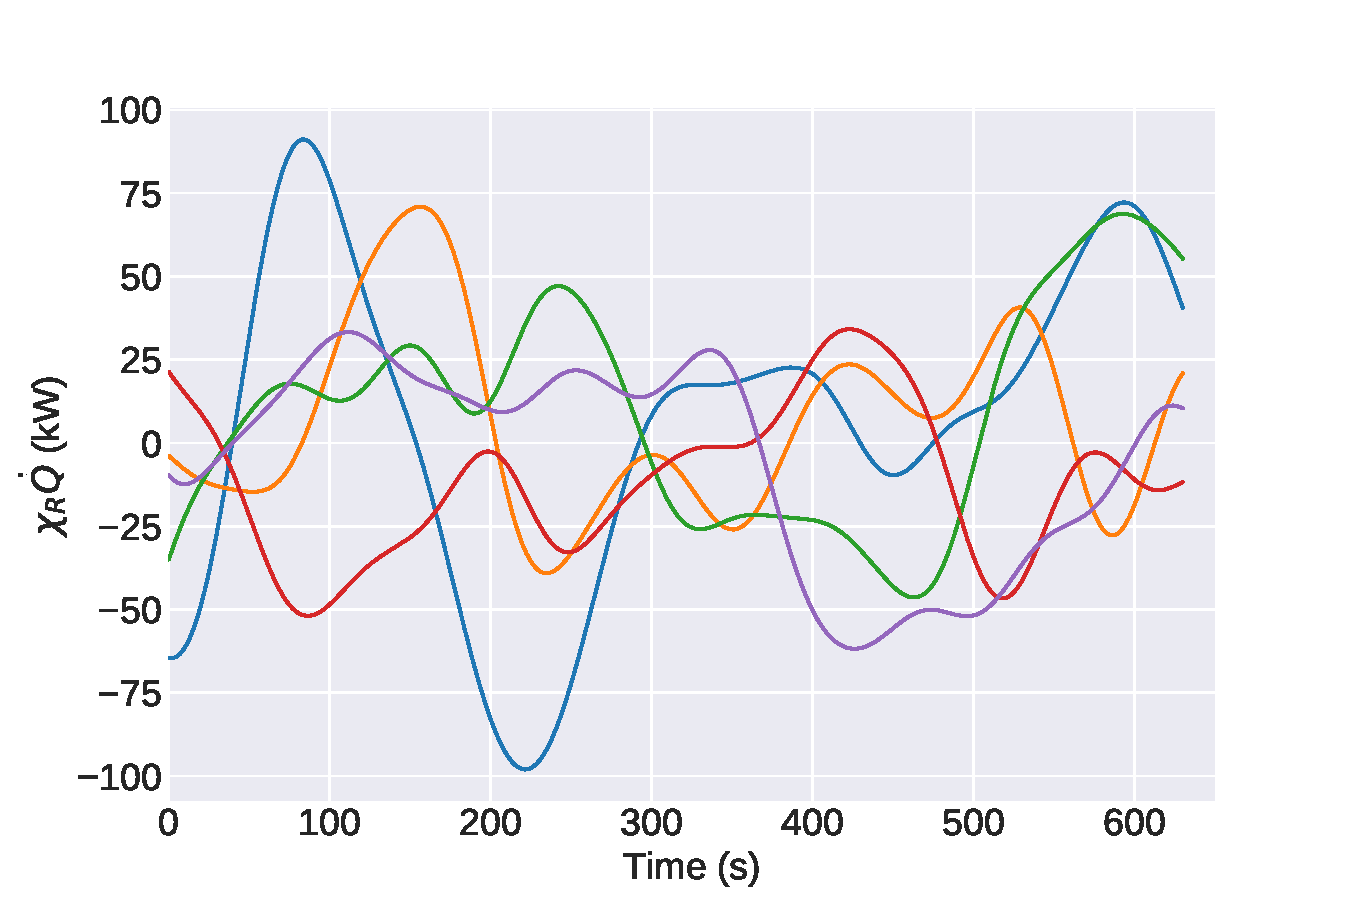
\includegraphics[width=\textwidth,keepaspectratio]{figures/gp_prior.pdf}
      \caption{Five draws from the prior with optimized hyperparameters.}
      \label{fig:gp_prior}
  \end{subfigure}
  \begin{subfigure}[t]{.45\textwidth}
      \centering
      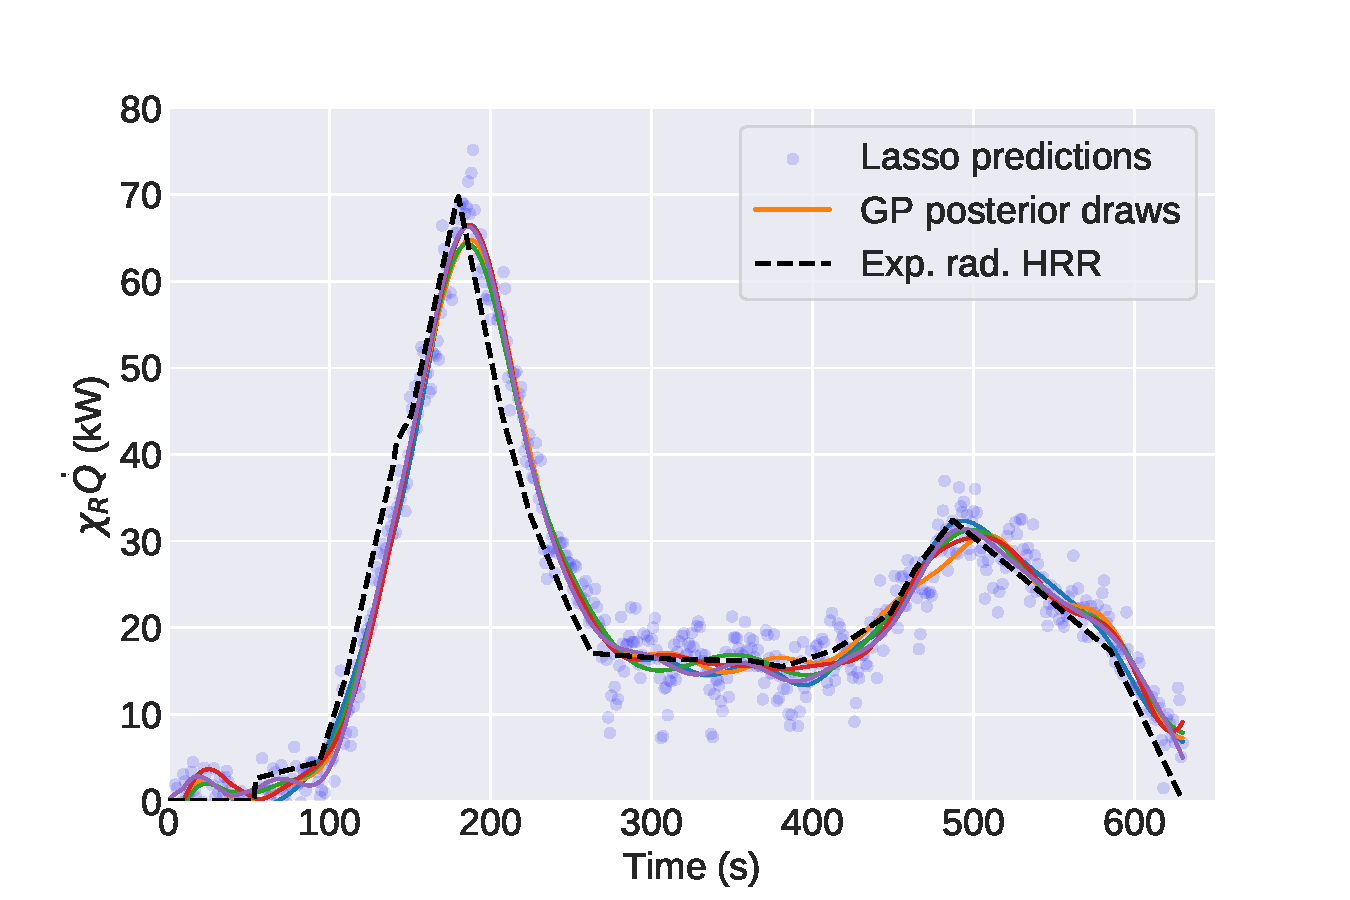
\includegraphics[width=\textwidth ,keepaspectratio]{figures/gp_posterior.pdf}
      \caption{Five draws from the posterior distribution.}
      \label{fig:gp_posterior}
  \end{subfigure}
  \caption{A visual demonstration of the Gaussian process methodology. Figure \protect\ref{fig:gp_prior} shows five random draws from the Gaussian process prior with optimized hyperparameters. Using Bayes' law, the GPR methodology updates this distribution of functions given the lasso predictions. The resulting distribution of functions produces more accurate reconstructions of the true radiative HRR curve than the lasso model does by itself.} 
  \label{fig:gp_regression_example}
\end{figure}

In order to gain a better idea of the the ability of this framework to measure radiative HRR curves, the methodology described in this section is conducted four times with each of the four experiments serving as the test case once. The model trains on the other three experiments and predicts the HRR curve for the test experiment. These results are shown in Figure \ref{fig:dft_gp_results}.

\begin{figure}[htbp]
  \centering
  \begin{subfigure}[t]{.45\textwidth}
      \centering
      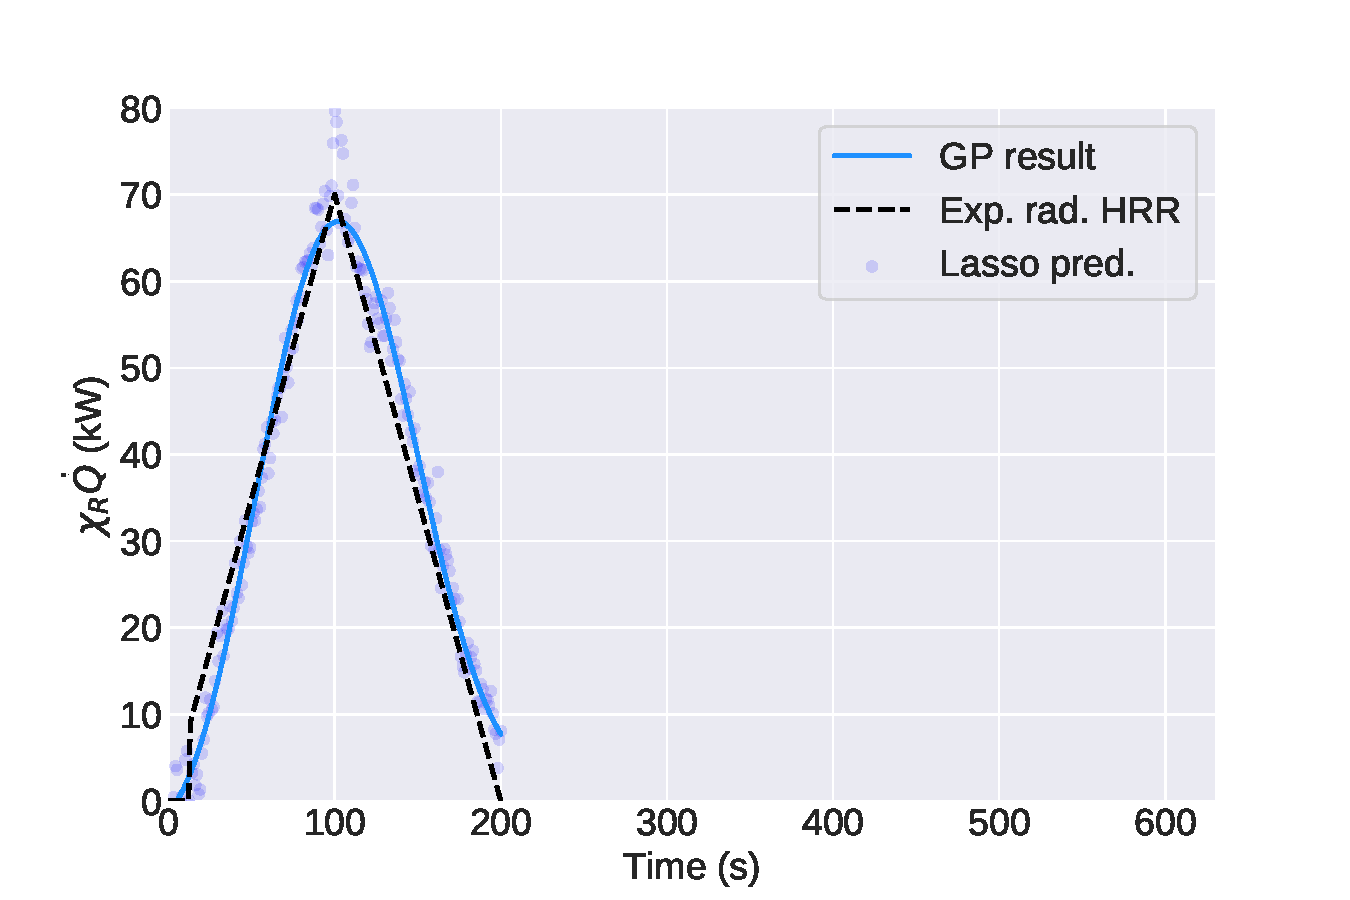
\includegraphics[width=\textwidth,keepaspectratio]{figures/dft_result_100s_triangle.pdf}
      \caption{100 sec. triangle}
      \label{fig:dft_result_100s_triangle}
  \end{subfigure}
  \begin{subfigure}[t]{.45\textwidth}
      \centering
      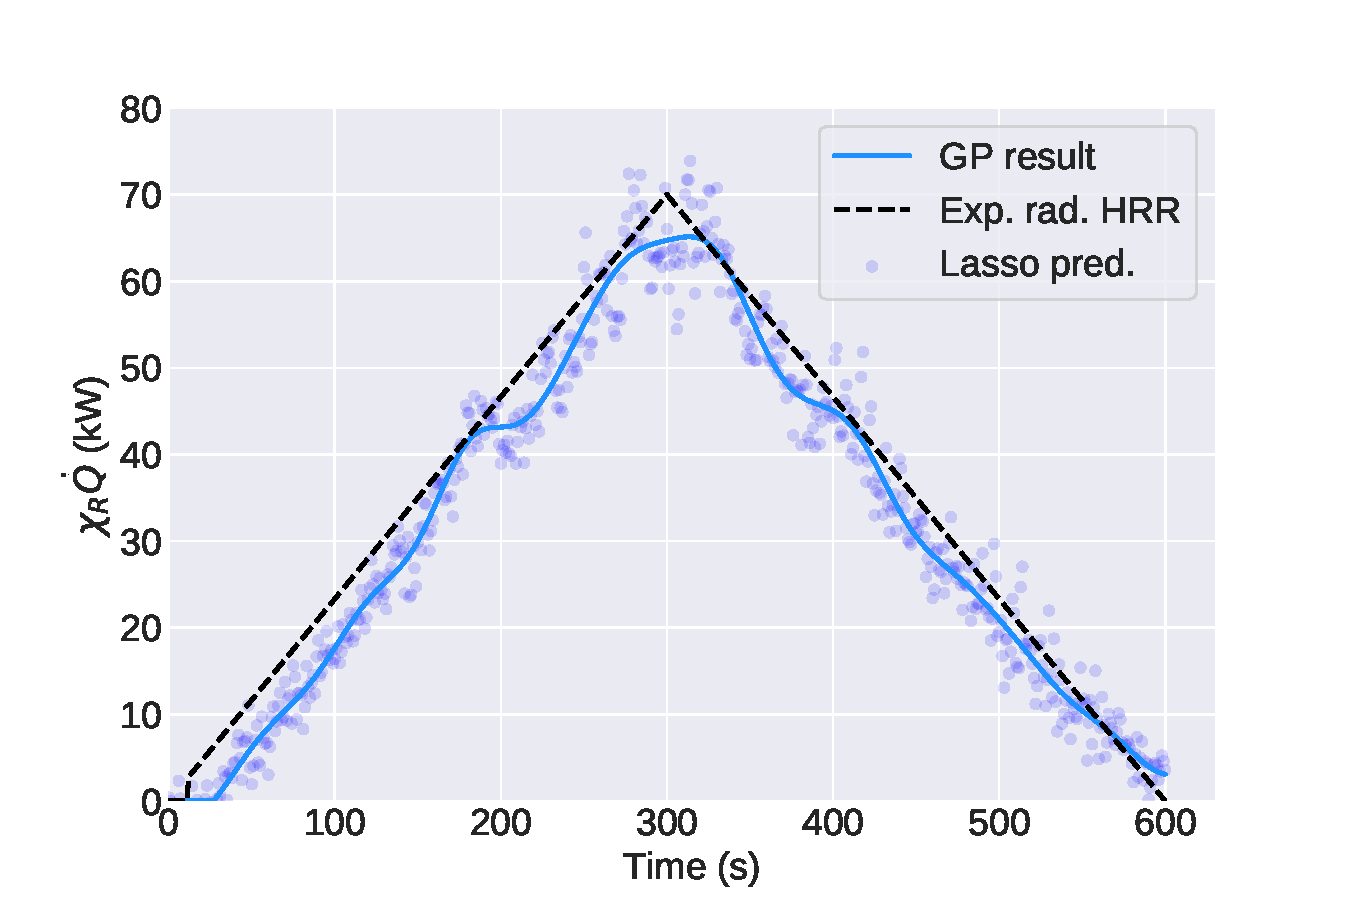
\includegraphics[width=\textwidth ,keepaspectratio]{figures/dft_result_300s_triangle.pdf}
      \caption{300 sec. triangle}
      \label{fig:dft_result_300s_triangle}
  \end{subfigure}
   \begin{subfigure}[t]{.45\textwidth}
      \centering
      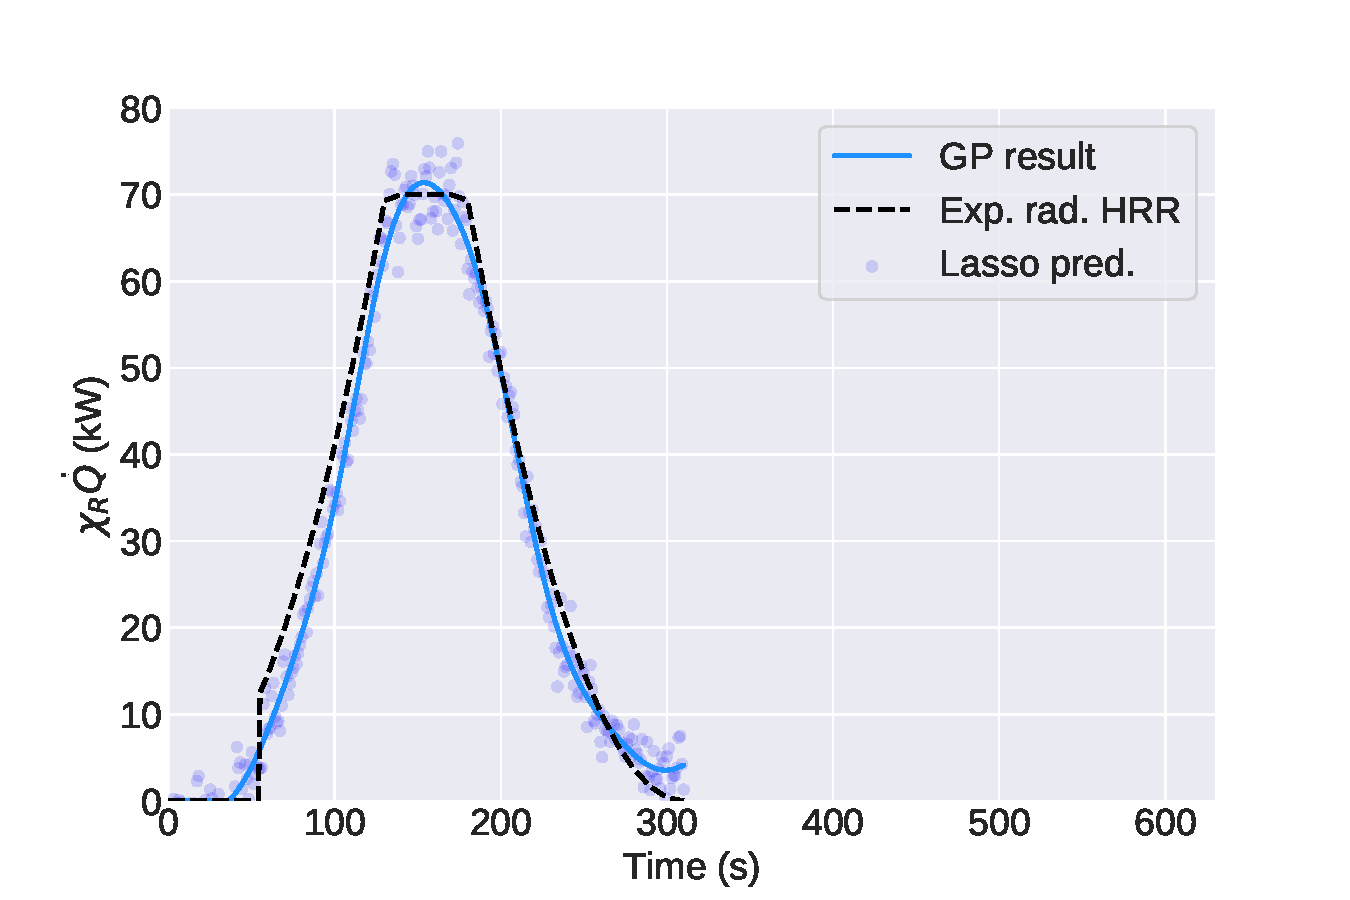
\includegraphics[width=\textwidth ,keepaspectratio]{figures/dft_result_t_squared.pdf}
      \caption{t-squared}
      \label{fig:dft_result_t_squared}
  \end{subfigure}
    \begin{subfigure}[t]{.45\textwidth}
      \centering
      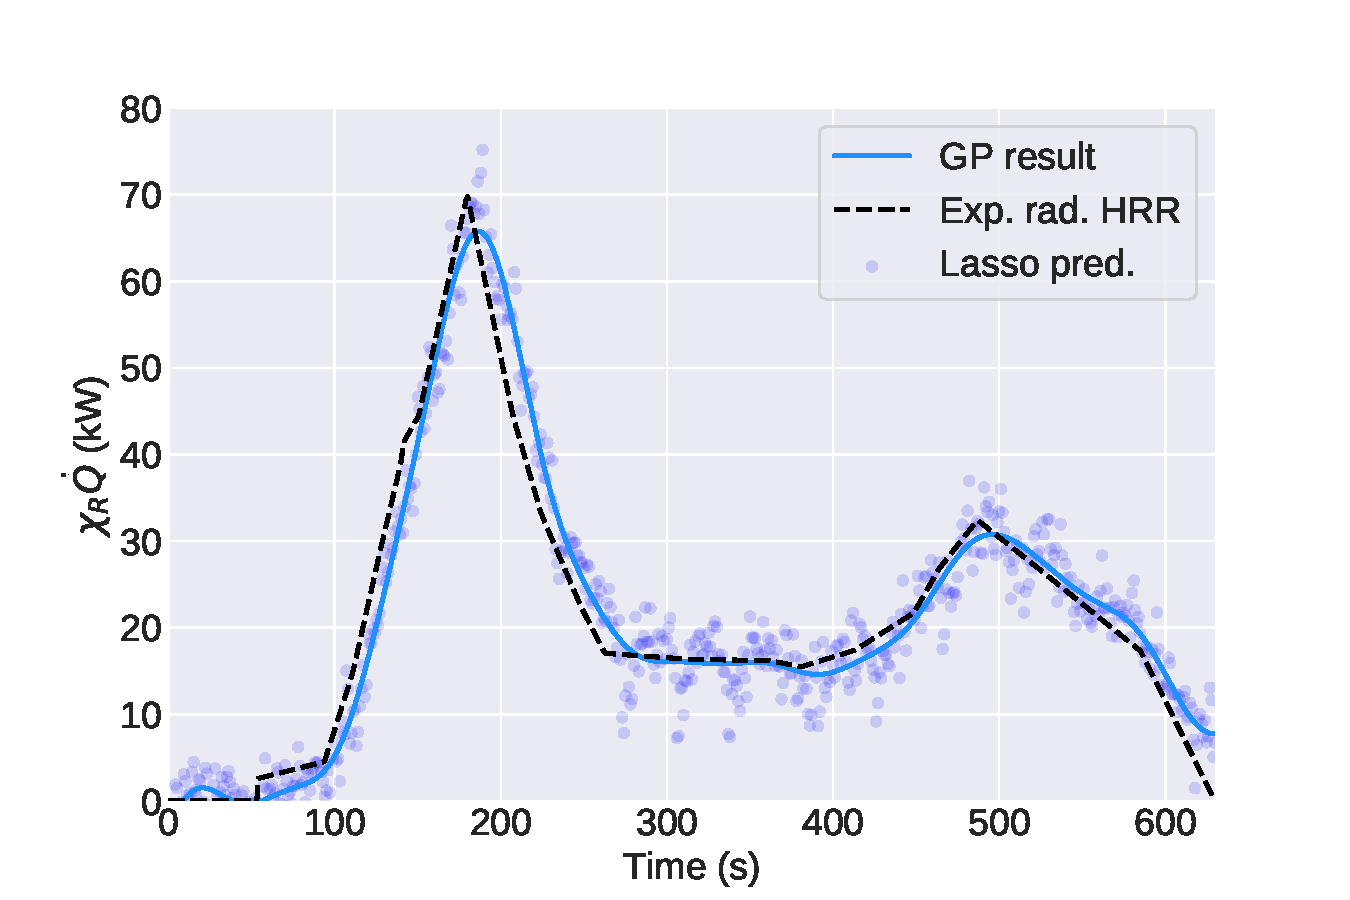
\includegraphics[width=\textwidth ,keepaspectratio]{figures/dft_result_weird_curve.pdf}
      \caption{Arbitrary ramp}
      \label{fig:dft_result_weird_curve}
  \end{subfigure}
  \caption{A demonstration of the methodology described in this section for each of the four burner experiments. For each experiment, the model trains on the other three experiments and predicts the radiative HRR ramp of the excluded experiment. Although the Lasso model produces noisy estimates, the Gaussian process regression is able to use the lasso predictions to make more accurate predictions.} 
  \label{fig:dft_gp_results}
\end{figure}



\clearpage
\subsection{Video analysis}
This section explores another machine learning approach for predicting the radiative heat release rate of a fire, which relies on analyzing video footage of the fire. The radiative heat release rate is specified because the approach is likely sensitive to the radiative fraction of the fuel burned. Nevertheless, this approach is likely the easiest to implement of the models described in the paper because it does not require any sensors besides a video camera and some method of producing fires with known HRR ramps for calibration. 

The central idea of this model is that the flame is expected to grow with increasing $\dot{Q}$. Using a video camera in a fixed location, a video of each burner experiment was collected. One frame was extracted as an image for every second of footage. The images were then reshaped into a 256 by 256 matrix of pixels. An example of these reshaped images is shown in Figure \ref{fig:fire_image}. Each pixel is described as a vector of length 3, with the entries describing the intensities of green, blue, and red light respectively on a scale from 0 to 255. In order to aggregate the three values into a single measure for each pixel, a ``normalized" intensity is calculated according to equation \ref{eqn:normalized_intensity},  

\begin{equation}
  \label{eqn:normalized_intensity}
 \text{Normalized intensity} = \frac{G + B + R}{(255)(3)}
\end{equation}

\noindent where $G$, $B$, and $R$ are the intensities of green, blue, and red light respectively. The denominator makes it so that the normalized intensity is on a scale between 0 and 1. Figure \ref{fig:brightness_heatmap} shows an example of a heatmap of the normalized intensity for an individual frame. Finally, a simple criterion is imposed to isolate the flame area. If the normalized intensity of a pixel is above 0.99, that pixel is assigned a value of 1; otherwise it is set to zero. Figure \ref{fig:binary_fire_image} shows the resulting binary map of this approach with the white region showing pixels that are above 99\% of the maximum normalized intensity and the black region showing all other pixels. 


\begin{figure}[htbp]
  \centering
  \begin{subfigure}[t]{.35\textwidth}
      \centering
      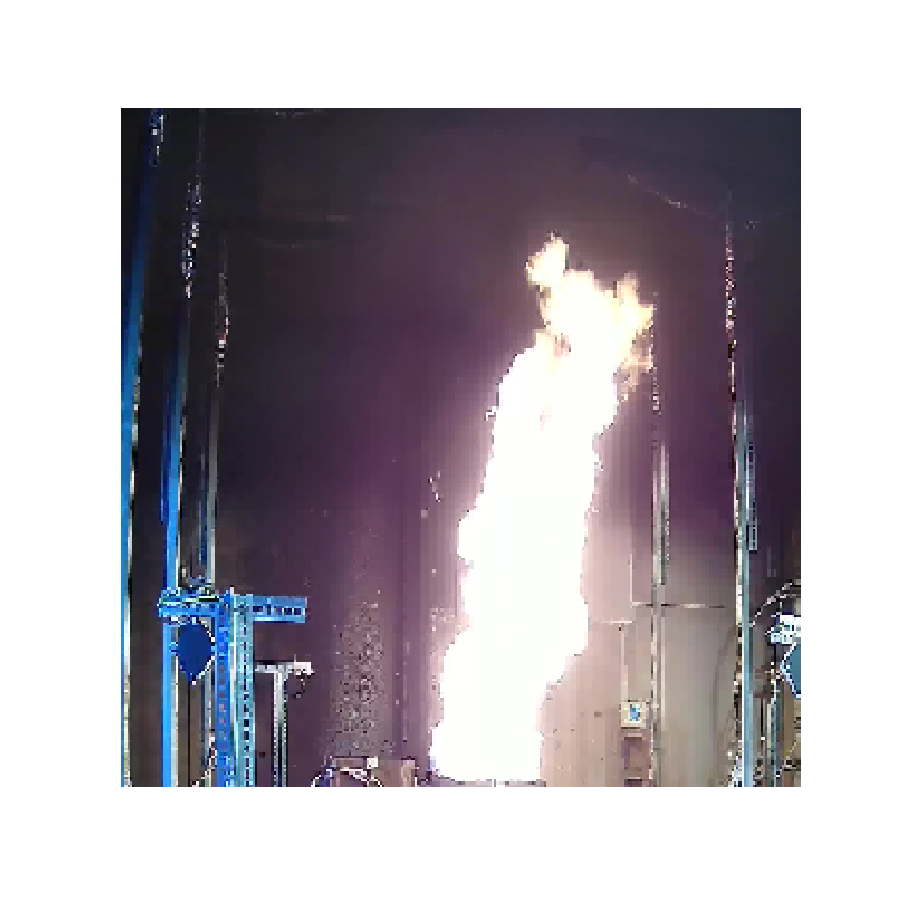
\includegraphics[width=\textwidth,keepaspectratio]{figures/fire_image.pdf}
      \caption{A resized (256x256) image of the fire from a frame of video footage.}
      \label{fig:fire_image}
  \end{subfigure}
  \begin{subfigure}[t]{.4\textwidth}
      \centering
      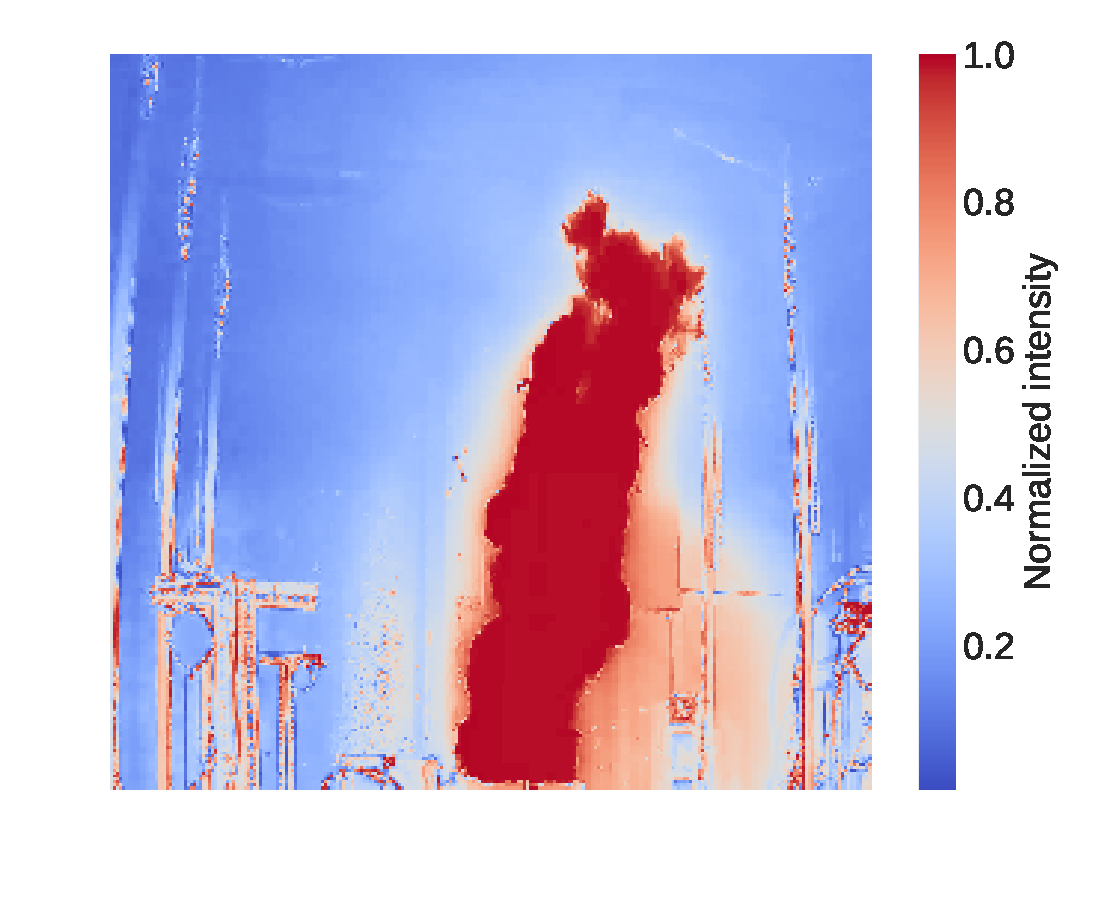
\includegraphics[width=\textwidth ,keepaspectratio]{figures/brightness_heatmap.pdf}
      \caption{Normalized intensity heatmap}
      \label{fig:brightness_heatmap}
  \end{subfigure}
  \begin{subfigure}[t]{.35\textwidth}
      \centering
      
\includegraphics[width=\textwidth ,keepaspectratio]{figures/binary_fire_image.pdf}
      \caption{Binary map identifying flame}
      \label{fig:binary_fire_image}
  \end{subfigure}
  \caption{Illustration of the video processing methodology. From the video, frames are extracted as 256x256 images such as the one shown in \protect\ref{fig:fire_image}. Each pixel has three intensity values which are aggregated into one value using equation \protect\ref{eqn:normalized_intensity} and this quantity is plotted as a heatmap in \protect\ref{fig:brightness_heatmap}. Finally, the pixels that have a normalized intensity above 0.99 are identified. These pixels are shown as white with all other pixels shown as black in \protect\ref{fig:binary_fire_image}.} 
  \label{fig:fire_image_processing}
\end{figure}

Next, the fraction, $f_{bright}$ of all pixels in the frame that are above 0.99 normalized intensity is computed. Figure \ref{fig:frac_bright} shows that the radiative heat release rate is correlated with this quantity, but there is non-linearity in the relationship. However, Figure \ref{fig:frac_bright_43} shows that $\dot{Q}_R = \chi_R\dot{Q}$ exhibits a fairly linear correlation with $f_{bright}^{4/3}$.


\begin{figure}[htbp]
  \centering
  \begin{subfigure}[t]{.45\textwidth}
      \centering
      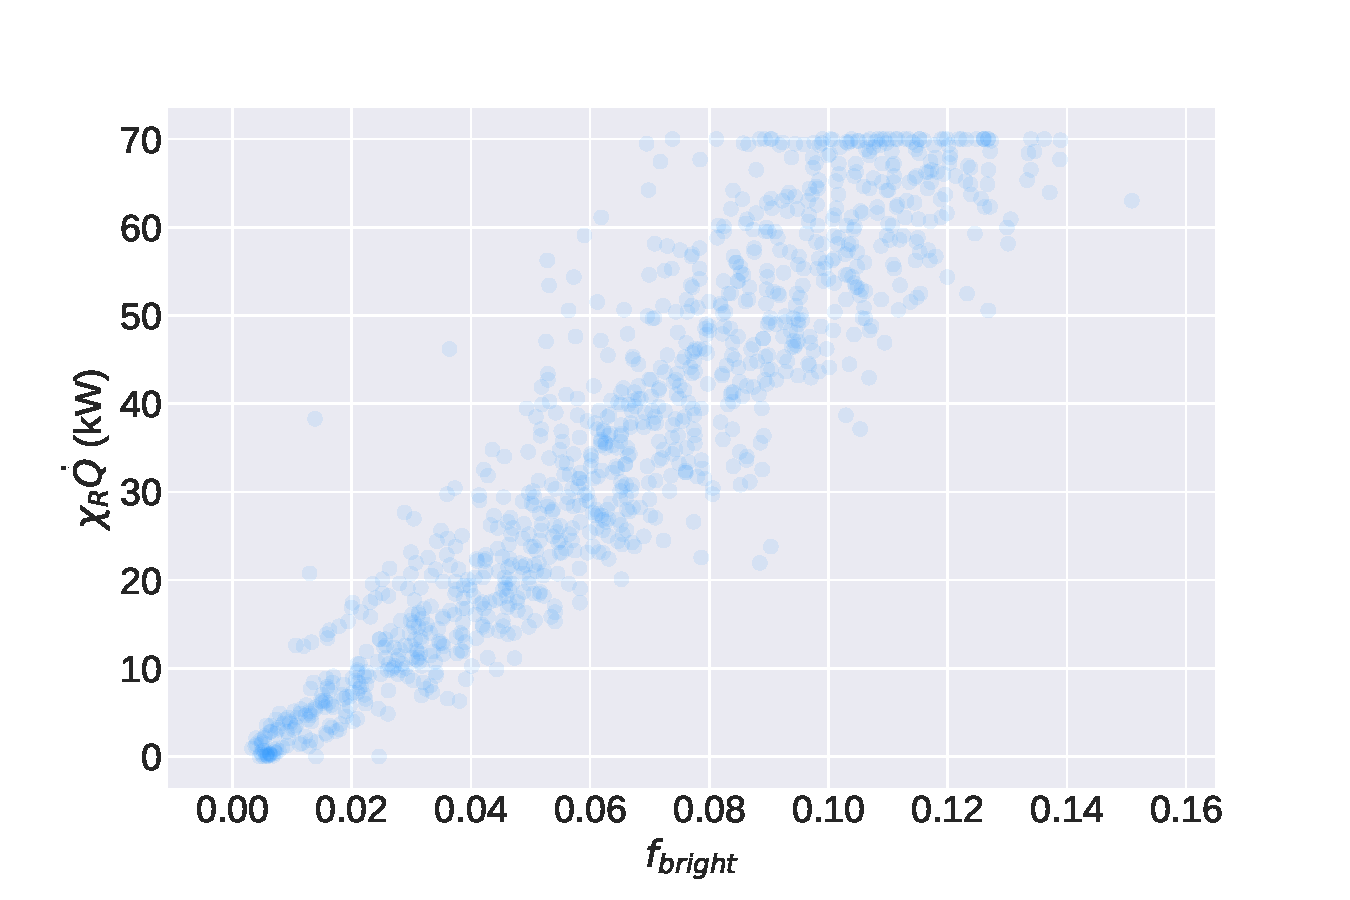
\includegraphics[width=\textwidth,keepaspectratio]{figures/frac_bright_scatterplot.pdf}
      \caption{}
      \label{fig:frac_bright}
  \end{subfigure}
  \begin{subfigure}[t]{.45\textwidth}
      \centering
      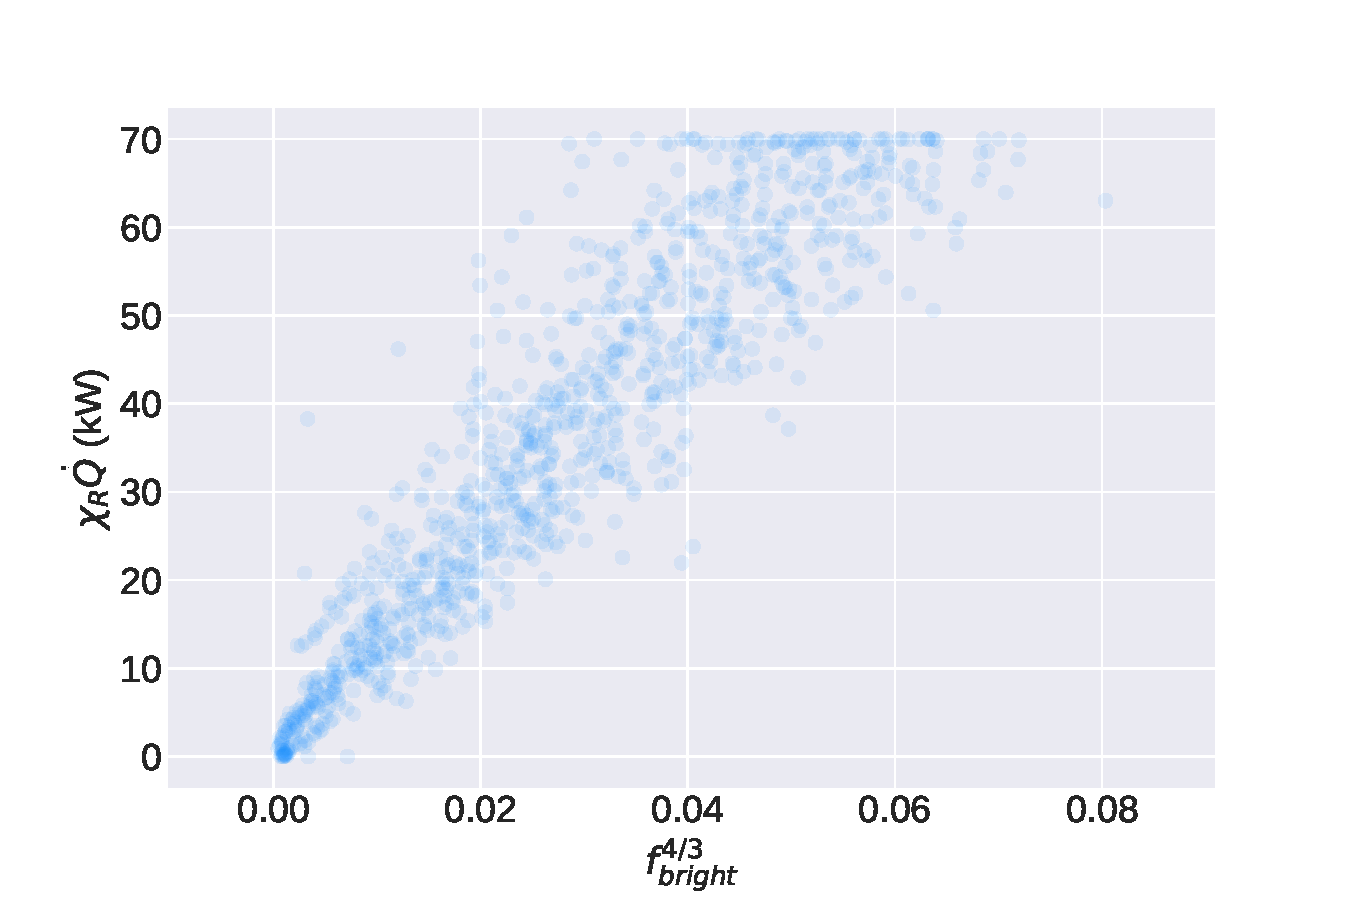
\includegraphics[width=\textwidth ,keepaspectratio]{figures/frac_bright_43_scatterplot.pdf}
      \caption{}
      \label{fig:frac_bright_43}
  \end{subfigure}
  \caption{Scatterplot showing the radiative heat release rate against the fraction of pixels with normalized intensities above 0.99 (\protect\ref{fig:frac_bright}). Raising $f_{bright}$ to the power of 4/3 appears to correct for the non-linearity in the relationship (\protect\ref{fig:frac_bright_43}).} 
  \label{fig:frac_bright_scatterplots}
\end{figure}


The linear correlation motivates the use of a simple linear regression, whose form is specified in equation 

\begin{equation}
  \label{eqn:bright_linear_regression}
 \dot{Q_R} = f_{bright}^{4/3}\beta
\end{equation}

The Gaussian process methodology described in the previous section is then repeated using the predictions from the simple regression model in place of the predictions from the lasso model with the heat flux measurements. The predictions of $\dot{Q}_R$ for each of the four experiments is shown in Figure \ref{fig:image_results}.

\begin{figure}[htbp]
  \centering
  \begin{subfigure}[t]{.45\textwidth}
      \centering
      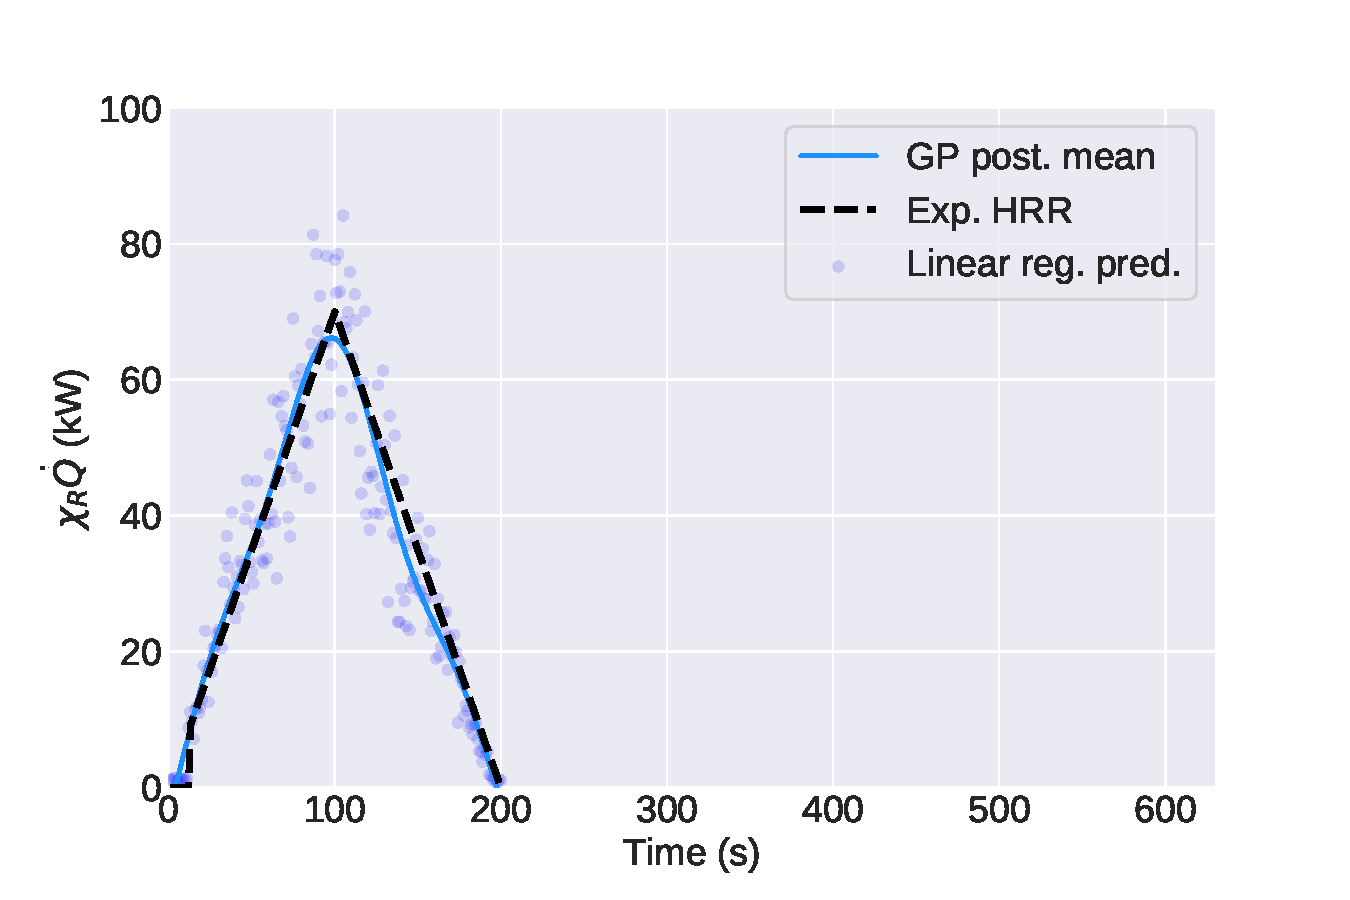
\includegraphics[width=\textwidth,keepaspectratio]{figures/image_result100s_triangle.pdf}
      \caption{100 second triangle}
      \label{fig:image_result_100s_triangle}
  \end{subfigure}
  \begin{subfigure}[t]{.45\textwidth}
      \centering
      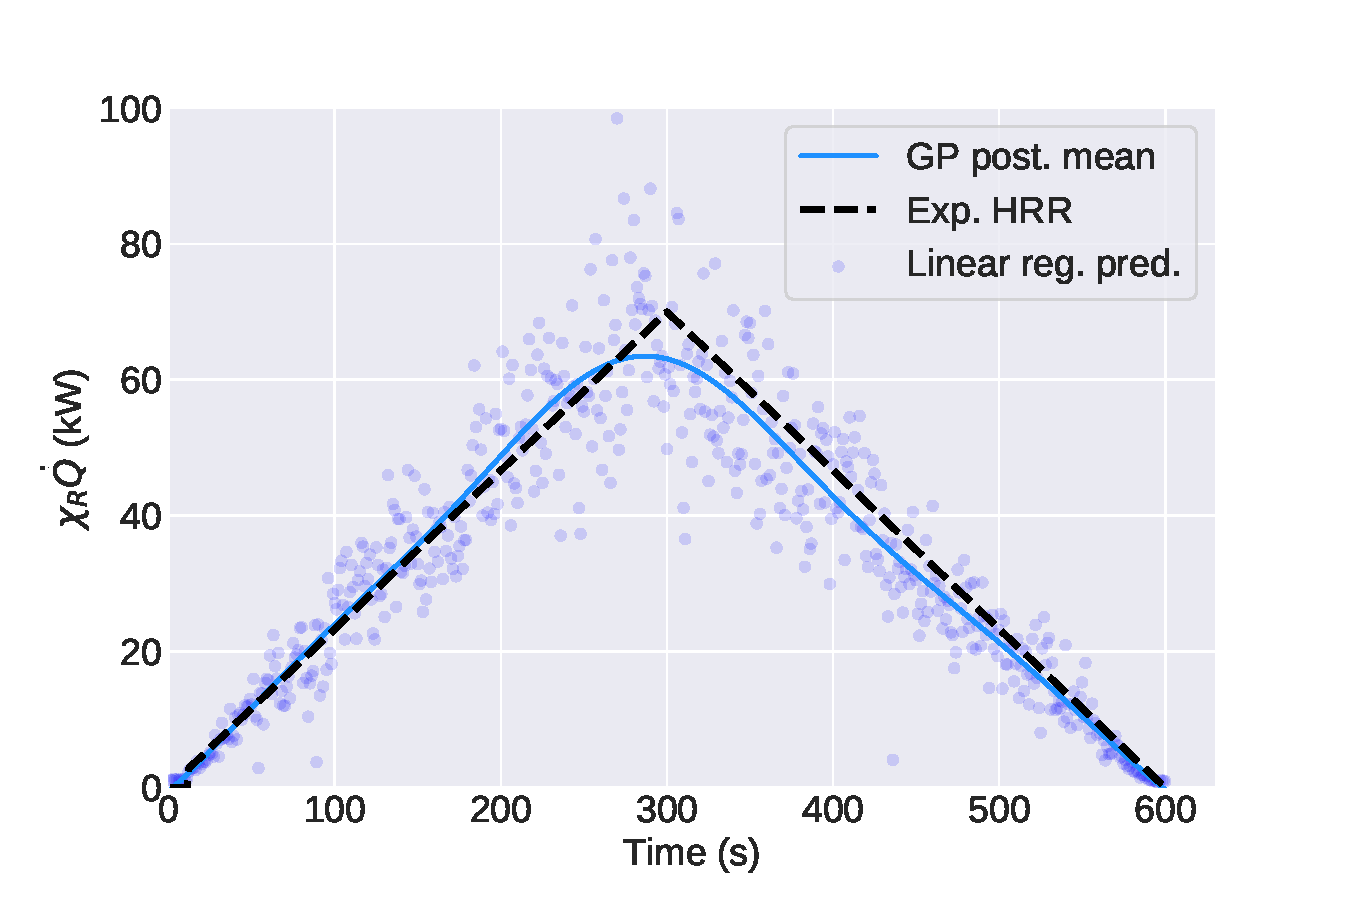
\includegraphics[width=\textwidth ,keepaspectratio]{figures/image_result300s_triangle.pdf}
      \caption{300 second triangle}
      \label{fig:image_result_300s_triangle}
  \end{subfigure}
   \begin{subfigure}[t]{.45\textwidth}
      \centering
      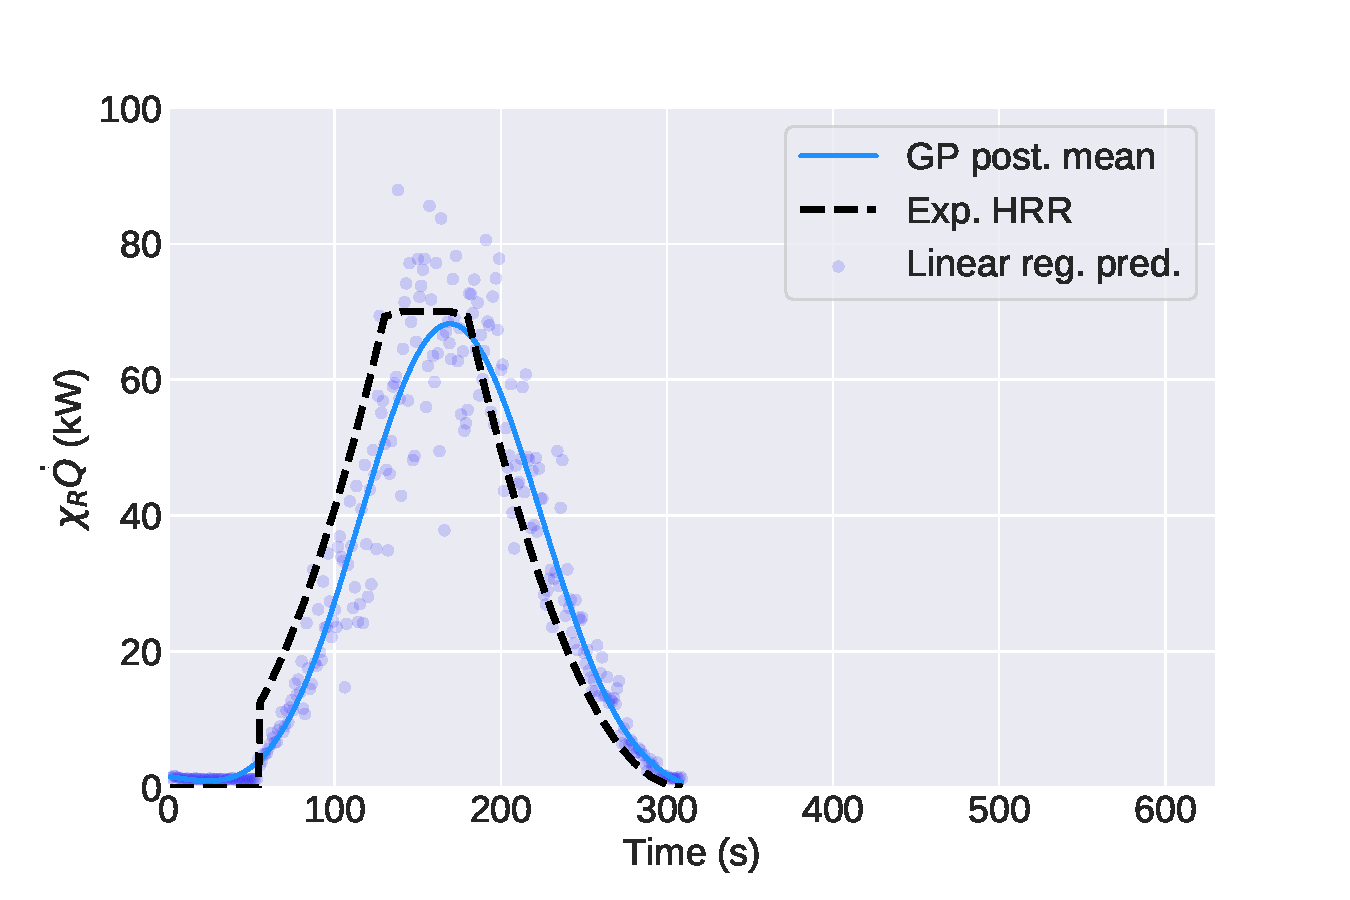
\includegraphics[width=\textwidth ,keepaspectratio]{figures/image_resultt_squared.pdf}
      \caption{t-squared}
      \label{fig:image_result_t_squared}
  \end{subfigure}
    \begin{subfigure}[t]{.45\textwidth}
      \centering
      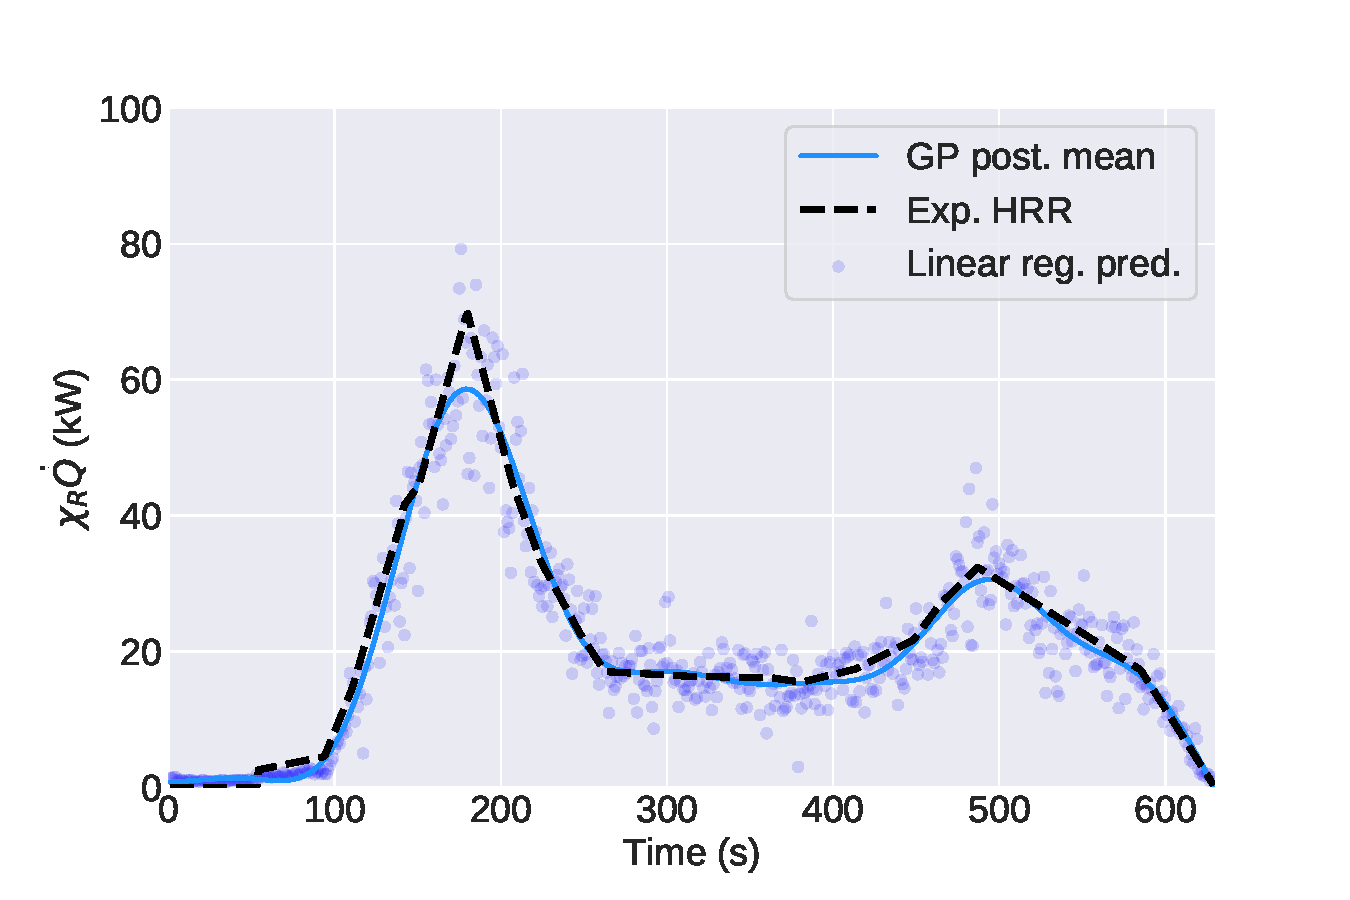
\includegraphics[width=\textwidth ,keepaspectratio]{figures/image_resultweird_curve.pdf}
      \caption{Arbitrary ramp}
      \label{fig:image_result_weird_curve}
  \end{subfigure}
  \caption{The predicted radiative HRR curve for each of the four burner experiments using the video analysis methodology described in this section. Again, for each of the four tests, the model is trained on the three other tests only.} 
  \label{fig:image_results}
\end{figure}

The results of this methodology appear to vary significantly across the four burner experiments. The linear regression predictions appear to be noisier than the lasso model used on the heat flux measurements, but interestingly the Gaussian process predicts the radiative HRR more accurately than its counterpart described in the previous section, at least for the triangle fires and the arbitrary ramp fire. The predictions in the t-squared fire appear to lag behind the actual radiative HRR, though it is not clear why. The burner ignited the latest in this experiment of the four (~50 fixthis seconds), but one would expect that a framework based on video analysis would not exhibit time lag effects. 


\clearpage
\subsection{Thermocouple measurements}
In this section, various models are presented for predicting the heat release rate of a fire based on a set of thermocouple measurements. The models presented in the previous sections are assumed to depend signficantly on the radiative fraction, $\chi_R$ of the fuel, and therefore are assumed to provide insight into the the radiative component of the heat release rate, $\chi_R$, rather than the total heat release rate, $\dot{Q}$. Ideally, the temperatures can provide information on $\dot{Q}_R$ regardless of $\chi_R$, making the calorimetry framework robust to differences in fuels. To examine if this is the case, a sensitivity analysis was conducted to examine how much varying $\chi_R$ affects the thermocouple responses. This was done by running 10 different FDS cases modeling the experimental setup. For all cases, the total HRR ramp was a symmetric triangle fire with a peak HRR of 200 kW and a 200 second time to peak. However, $\chi_R$ was varied from 0 to 0.40 in the simulations. The results are shown in Figure \ref{fig:constant_Qtot_assumption}. 

\begin{figure}[htb] \centering
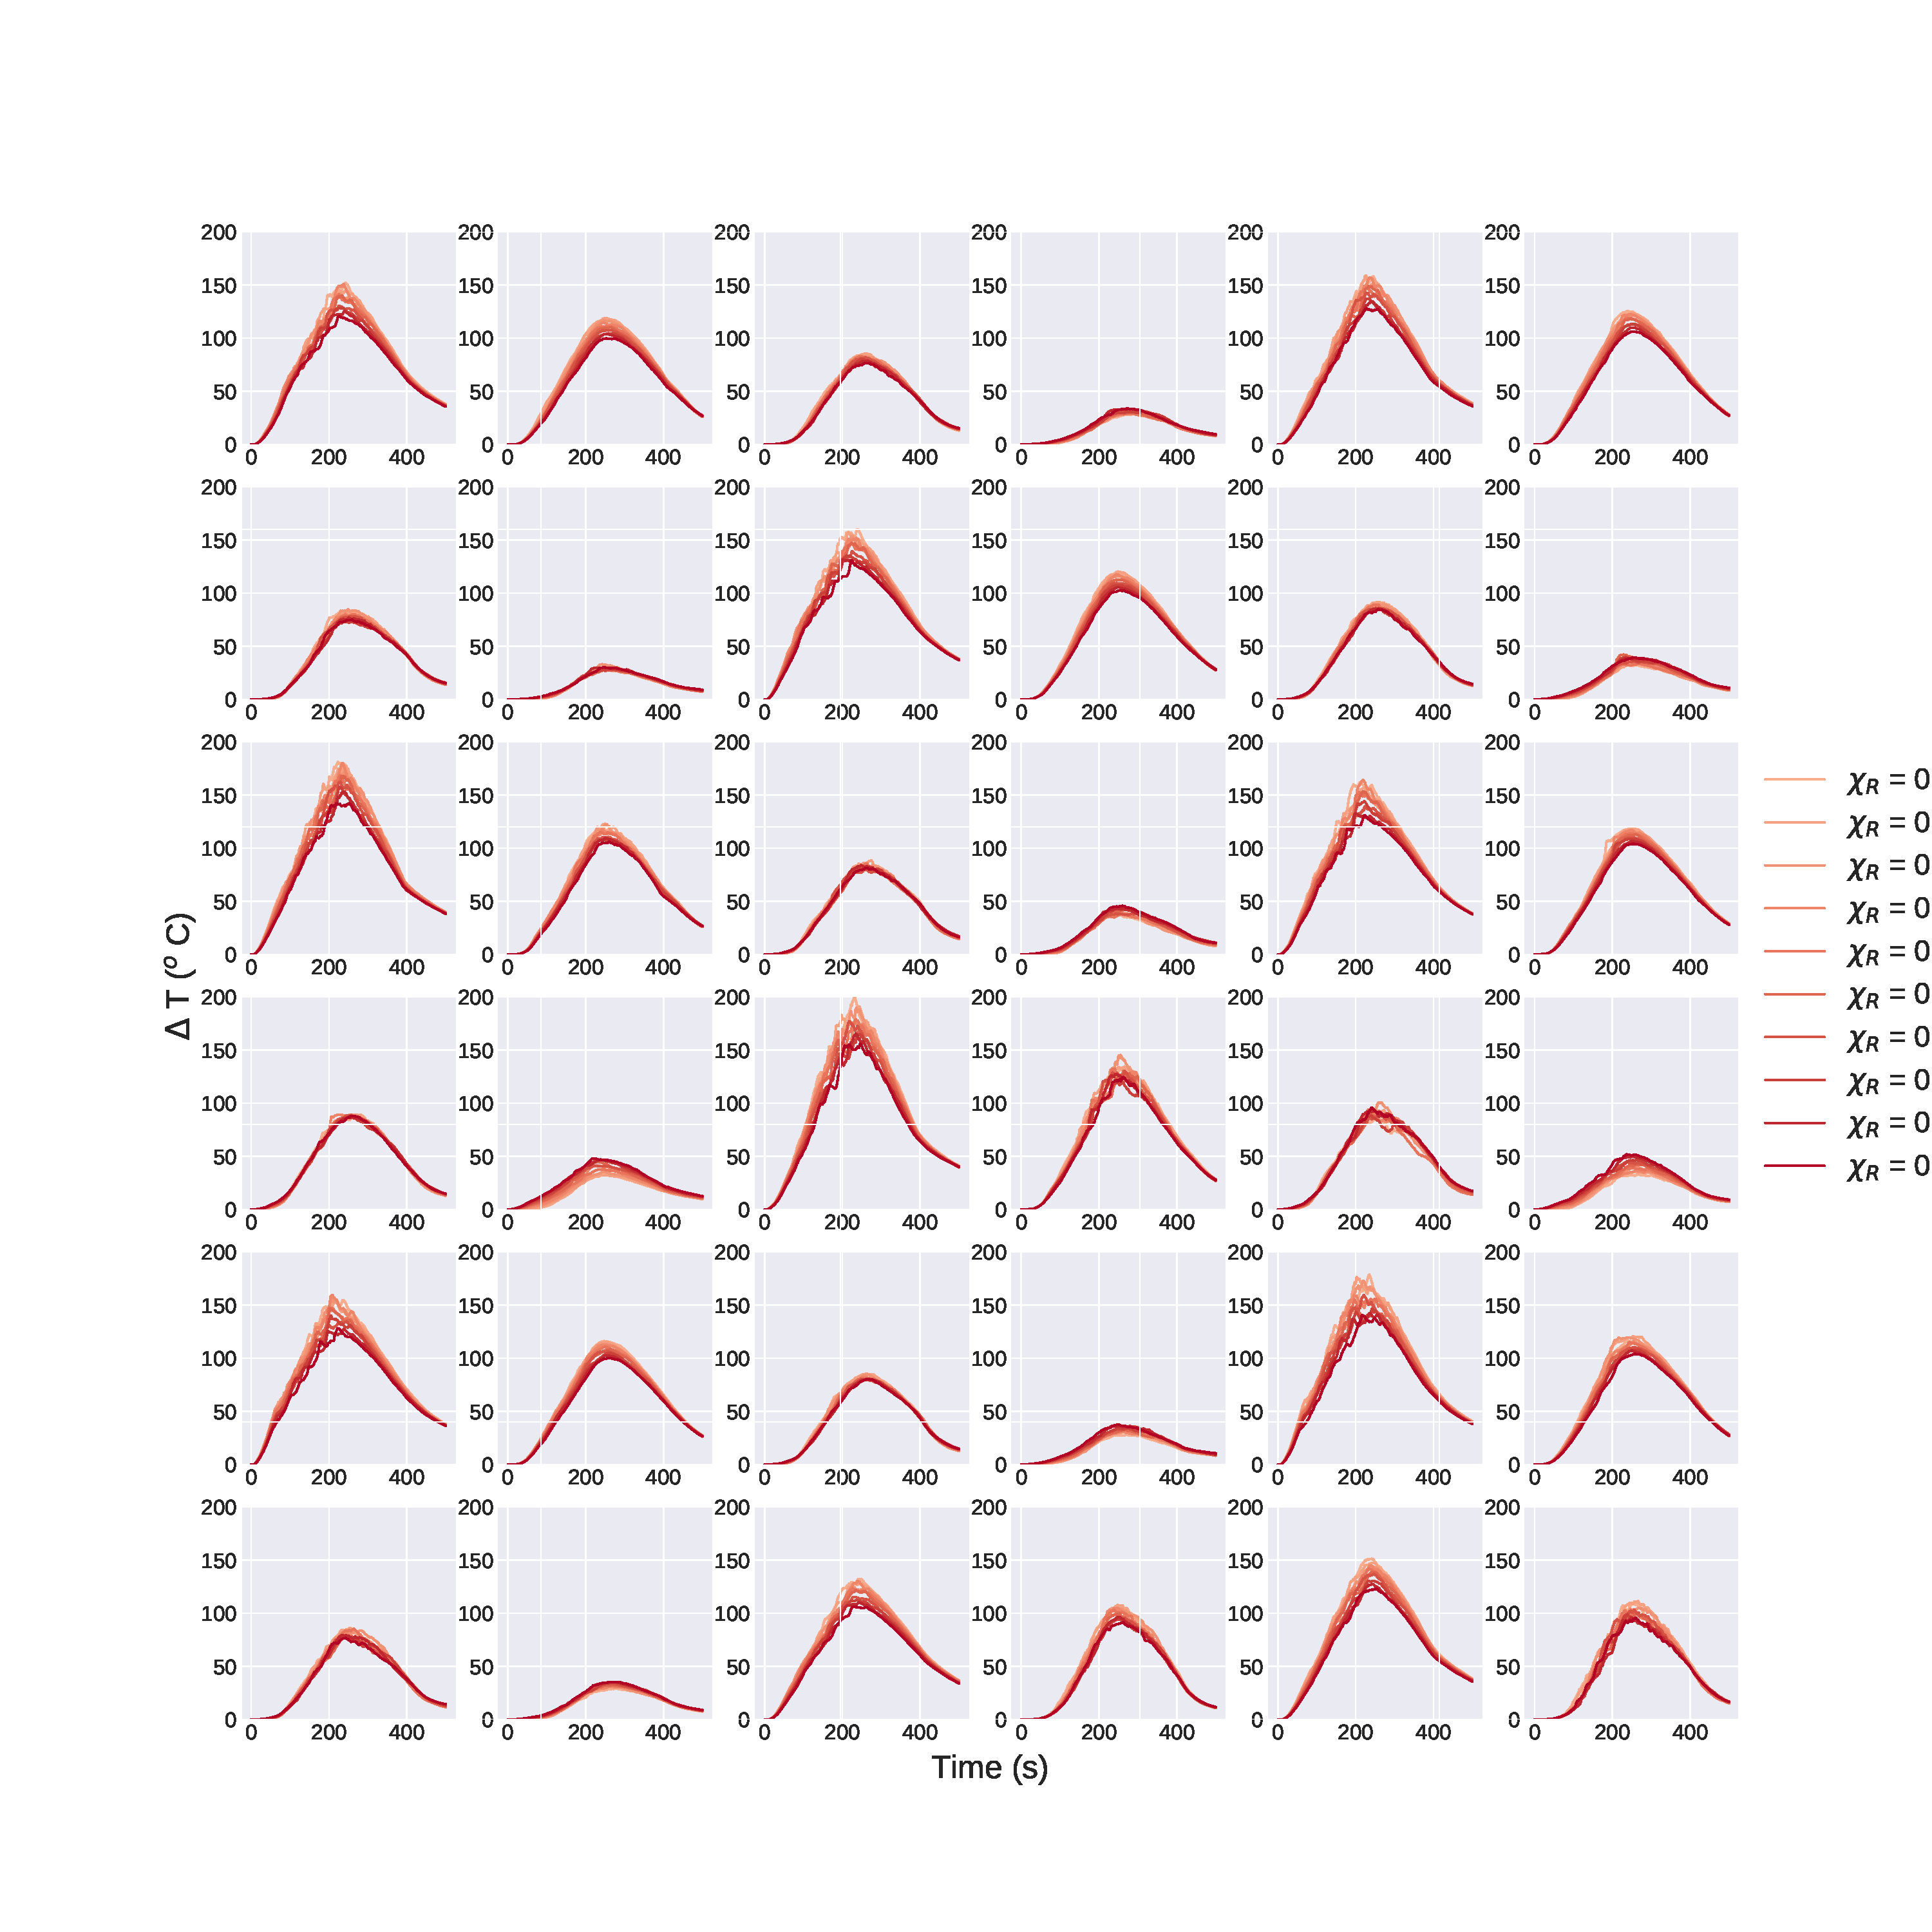
\includegraphics[width=.9\textwidth]{./figures/constant_Qtot_assumption.pdf}
\caption{A matrix of plots showing the sensitivity of the predicted thermocouple response to different radiative fractions, $\chi_R$. 10 different FDS cases were run and the total HRR ramp was the same across all cases; however, the radiative fraction was varied from $\chi_R = 0$ to $\chi_R=0.4$. The total HRR ramp for all cases is a symmetric triangle fire with a peak HRR of 200 kW that reaches the peak in 200 seconds.}
\label{fig:constant_Qtot_assumption}
\end{figure}

The results indicate that the thermocouple responses are relatively insensitive to $\chi_R$. This is likely due to the fact that the thermocouples are heated from both convection and radiation, so when the total heat output from the fire is the same, they will experience a similar amount of heating irrespective of the contributions of the individual heat transfer modes. 

The next step is to explore the relationship between the temperature differences, $\Delta T$ measured by the thermocouples and $\dot{Q}$. A scatterplot such as the one shown in Figure \ref{fig:temp_scatter} serves as a useful starting point.  


\begin{figure}[htb] \centering
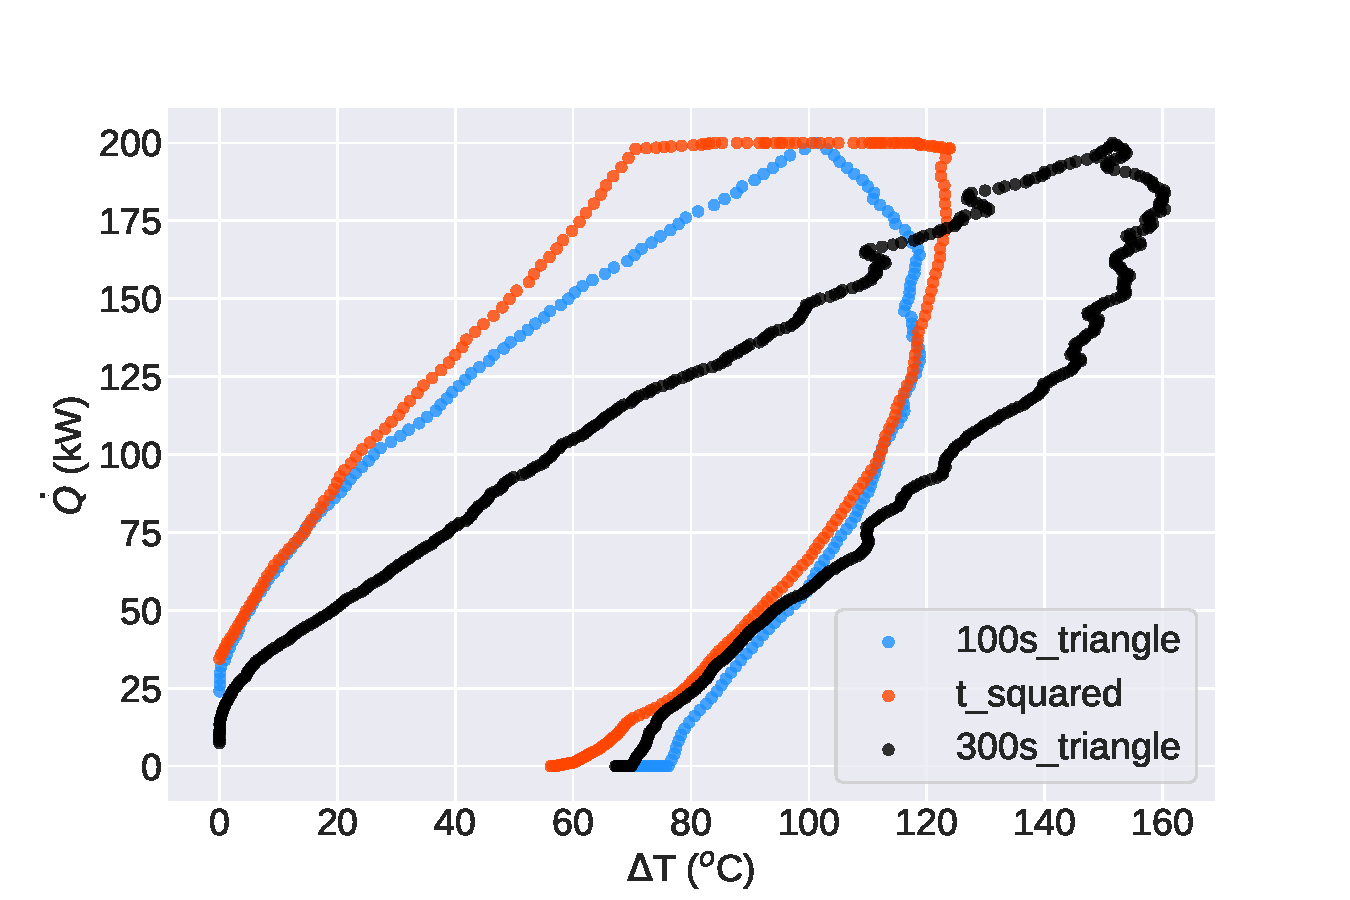
\includegraphics[width=.75\textwidth]{./figures/temp_scatter.pdf}
\caption{A scatterplot of the total heat release rate, $\dot{Q}$ vs. the experimentally measured $\Delta T$ of a single thermocouple. The result is typical of all other thermocouples and shows that the temperature response exhibits complex hysteresis that hinders the effectiveness of standard regression models. }
\label{fig:temp_scatter}
\end{figure}

Although the results shown in Figure \ref{fig:temp_scatter} are from only one of the 35 thermocouples that collected measurements during the experiments, the results are representative of the other sensors. Unlike the heat flux measurements, which show a linear relationship with $\dot{Q}$, the thermocouple measurements are characterized by complicated hysteretic paths that greatly hinder the use of ordinary statistical models. This is expected given the fact that the thermal masses of thermocouples make their measurements dependent on the history of surrounding gas temperatures and radiative heat fluxes. Furthermore, the surrounding gas temperature is also dependent on the fire's HRR history, meaning that the HRR cannot be reasonably inferred using only thermocouple measurements at an instant in time. These results motivate the use of physical models, which can predict a thermocouple's response as a time series given an HRR time series. FDS has this capability, but the simulations are computationally expensive and a HRR inversion framework can require many runs. The speed of the runs can be greatly improved by using coarser meshes at the potential expense of accuracy. In order to gain insight into which thermocouples are ideal for HRR inversion, two FDS simulations were run of the previously described 200 second triangle fire. In one simulation, the cells are 20 cm by 20 cm by 10 cm, and in the other they are 10 cm by 10 cm by 5 cm. The former case runs approximately eight times faster, but it is a relatively coarse mesh and may not full resolve the flow in some regions. Figure \ref{fig:grid_sensitivity} shows the results of these FDS simulations for the thermocouple locations used in the experiments.


\begin{figure}[htbp]
  \centering
  \begin{subfigure}[t]{.45\textwidth}
      \centering
      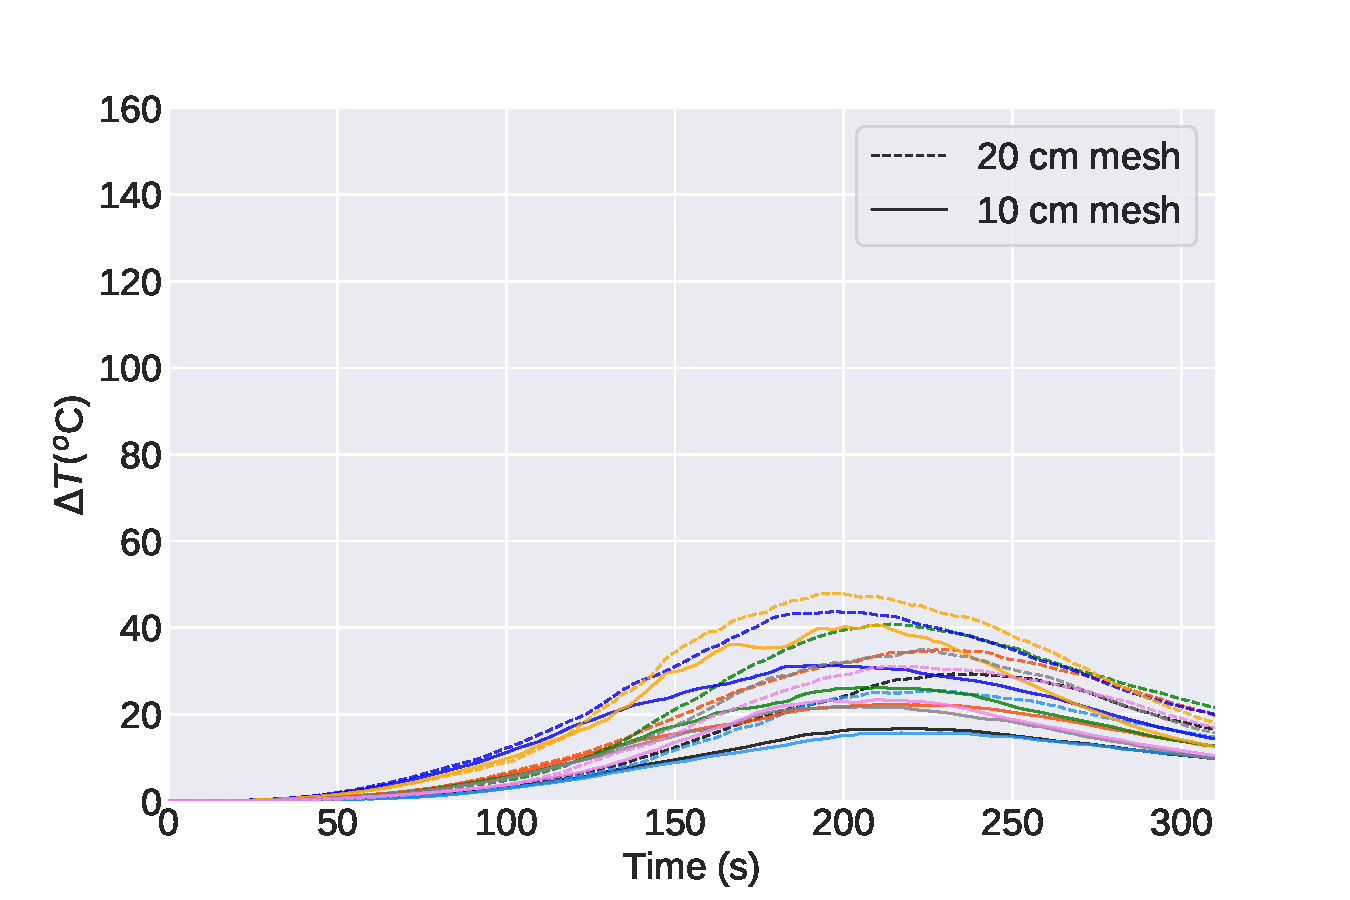
\includegraphics[width=\textwidth,keepaspectratio]{figures/053mesh_sensitivity.pdf}
      \caption{0.53 m off ground}
      \label{fig:0.53mesh_sensitivity}
  \end{subfigure}
  \begin{subfigure}[t]{.45\textwidth}
      \centering
      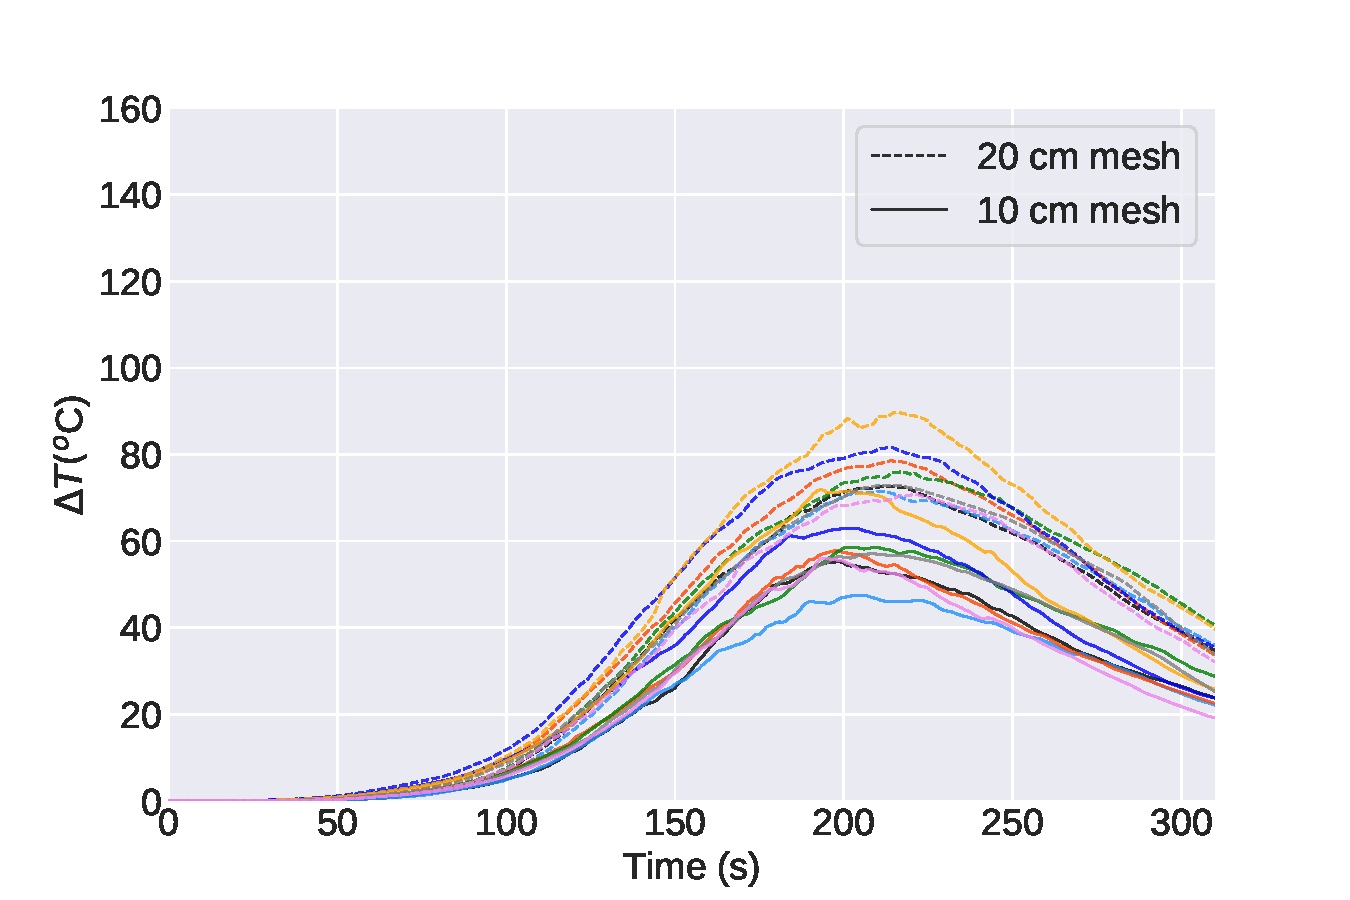
\includegraphics[width=\textwidth ,keepaspectratio]{figures/107mesh_sensitivity.pdf}
      \caption{1.07 m off ground}
      \label{fig:1.07mesh_sensitivity}
  \end{subfigure}
   \begin{subfigure}[t]{.45\textwidth}
      \centering
      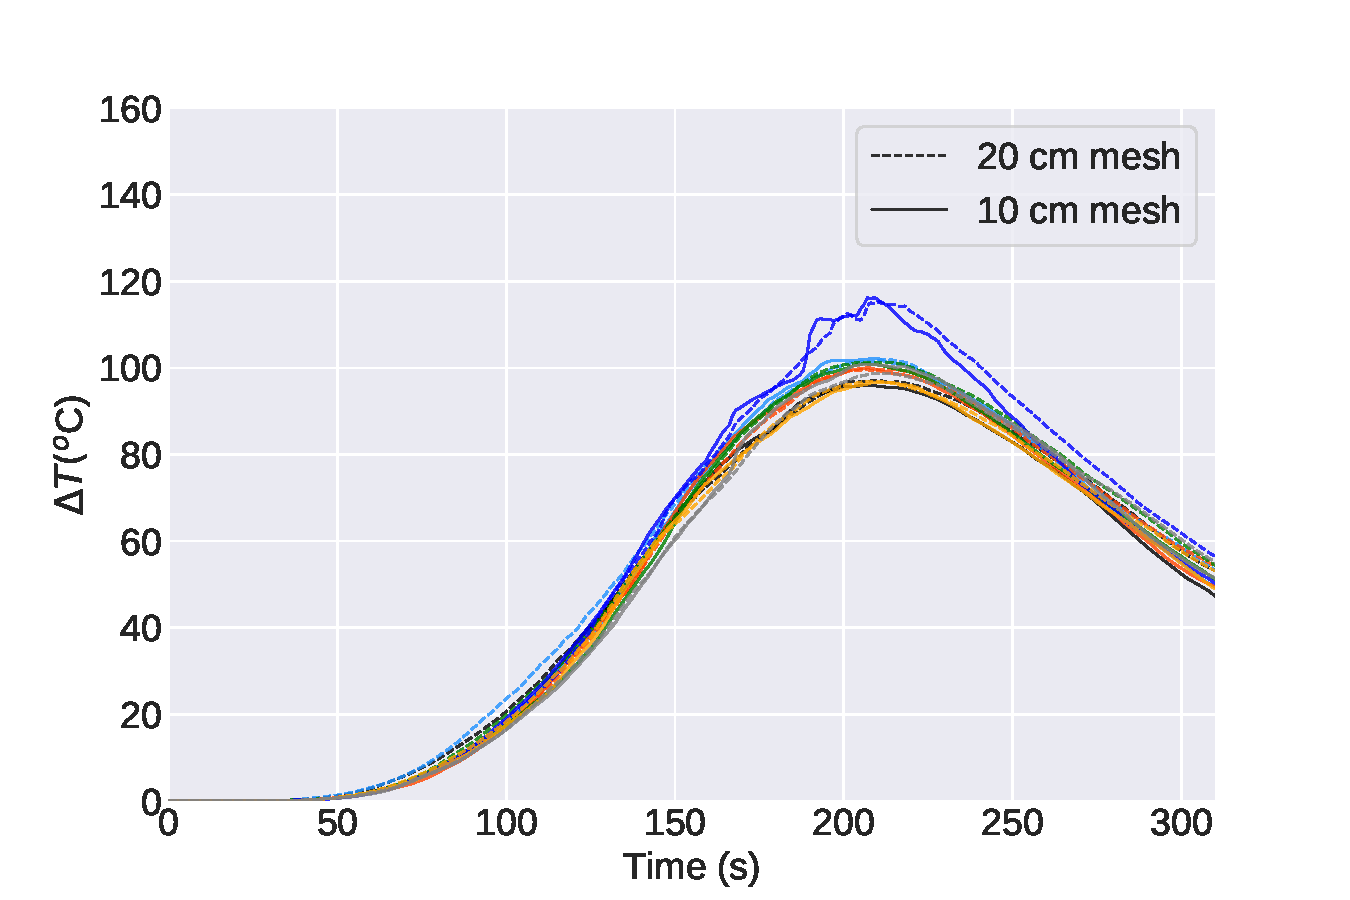
\includegraphics[width=\textwidth ,keepaspectratio]{figures/16mesh_sensitivity.pdf}
      \caption{1.6 m off ground}
      \label{fig:1.6mesh_sensitivity}
  \end{subfigure}
    \begin{subfigure}[t]{.45\textwidth}
      \centering
      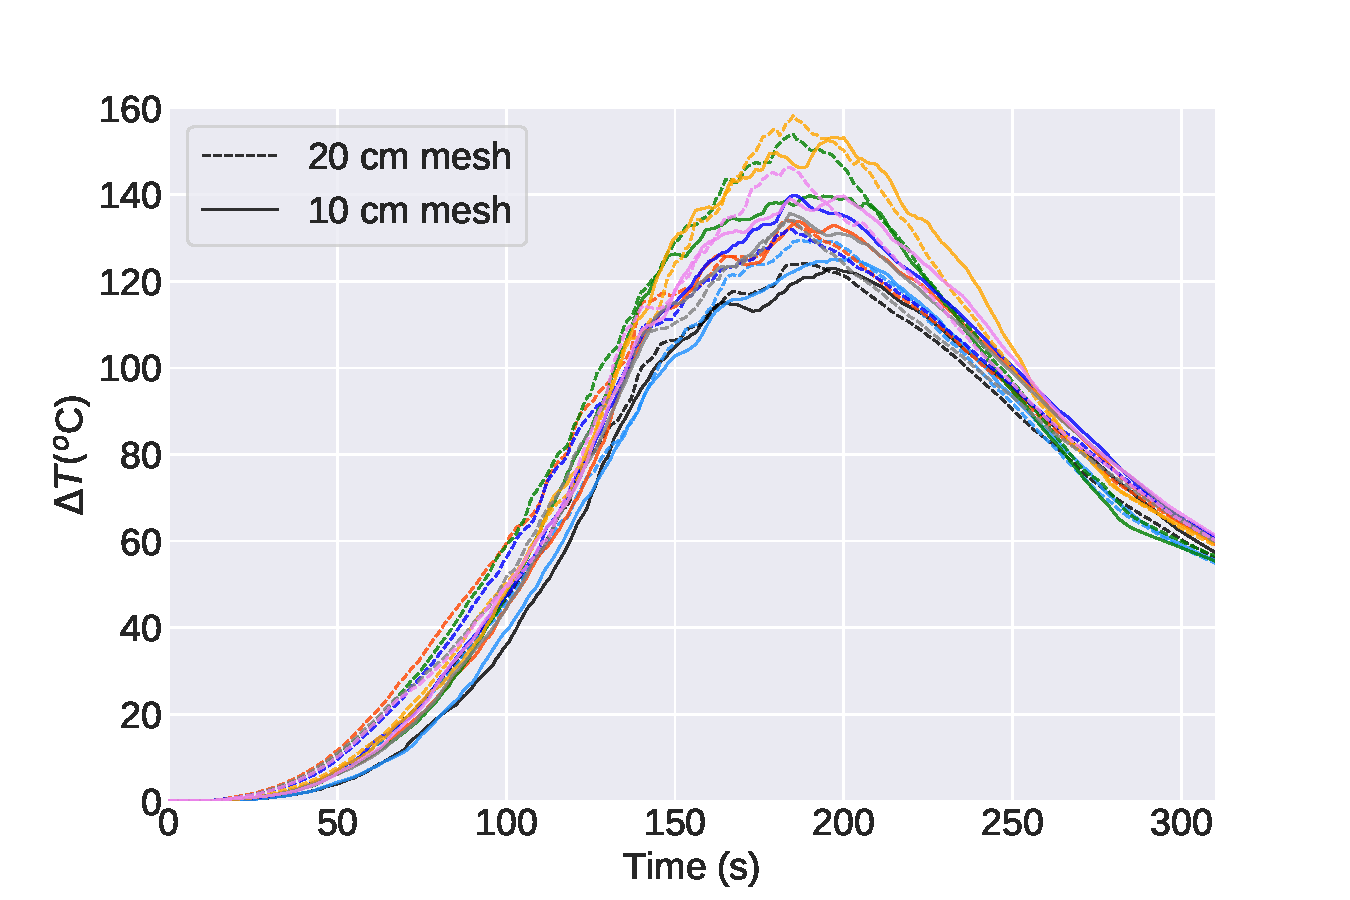
\includegraphics[width=\textwidth ,keepaspectratio]{figures/211mesh_sensitivity.pdf}
      \caption{2.1 m off ground}
      \label{fig:2.11mesh_sensitivity}
  \end{subfigure}
  \caption{The simulated responses of all thermocouples in the experiment using both a 10 cm x 10 cm x 5 cm mesh and a 20 cm x 20 cm x 10 cm mesh. The HRR ramp is the 100 second triangle fire previously described. The thermocouples are grouped by their heights off the ground. The results indicate that the thermocouples higher off the ground are both more sensitive to the HRR and less sensitive to the grid size, making them ideal for the HRR inversion framework.}
  \label{fig:grid_sensitivity}
\end{figure}


The ideal thermocouples are the ones whose measurements are the most sensitive to the quantity of interest, $\dot{Q}$, and the least sensitive to the use of a coarse mesh in FDS. Notice that the thermocouples that are 1.6 m off the ground or higher exhibit both of these figures of merit. As a result, these 17 thermocouples are used for the HRR inversion framework. 


\clearpage
\subsubsection{Forward FDS emulators}

Even with the coarse mesh, the FDS simulations can still be computationally expensive, taking nearly 30 minutes to run for one simulation, and many simulations can be required for inverse problems. Ideally, the inversion framework could provide nearly instantaneous estimates of the HRR using data collected from a new experiment without sacrificing accuracy. One way to accomplish this is to use emulators of FDS. These are machine learning models that learn the mapping between the input and the output of a physical model in order to circumvent the need for additional simulations. Specifically, an array of of artifical neural networks (ANN) is used to learn the mapping between a transient HRR $\dot{Q}(t)$ and an array of transient thermocouple responses, $\begin{bmatrix} \Delta T_1(t) & \Delta T_2(t) & \ldots & \Delta T_{17}(t) \end{bmatrix}$. A schematic of an emulator ANN is shown in Figure \ref{fig:neural_network_drawings} for a single thermocouple. 

\begin{figure}[htbp]
  \centering
  \begin{subfigure}[t]{.6\textwidth}
      \centering
      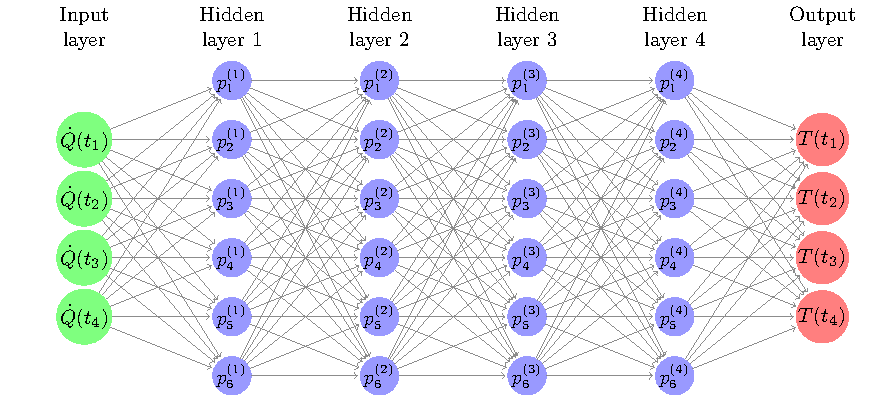
\includegraphics[width=\textwidth,keepaspectratio]{figures/neural_netowrk_diagram.pdf}
      \caption{A simplified diagram of the neural network   }
      \label{fig:neural_network_diagram}
  \end{subfigure}
  \begin{subfigure}[t]{.35\textwidth}
      \centering
      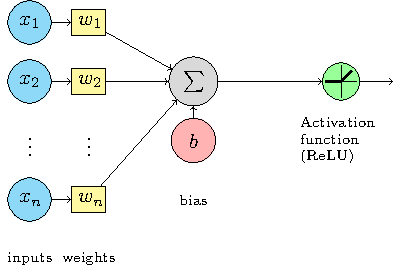
\includegraphics[width=\textwidth ,keepaspectratio]{figures/perceptron_diagram.pdf}
      \caption{}
      \label{fig:perceptron_diagram}
  \end{subfigure}
  \caption{\protect\ref{fig:neural_network_diagram} shows a simplified diagram of the neural network architecture used for each thermocouple response. In reality, the input layer and output layers each have 91 nodes as opposed to four, and each of the hidden layers has 128 perceptrons as opposed to six. The neural network is fully connected, meaning that each output of a given layer is an input to every perceptron in the next layer. \protect\ref{fig:perceptron_diagram} is a diagram showing the operation of an individual perceptron. All of the inputs to a given perceptron are weighted and then summed with an additional bias parameter. The result of this summation is sent through an activation function, which is the rectified linear activation function (ReLU) with the exception of the output layer, which simply outputs the sum.} 
  \label{fig:neural_network_drawings}
\end{figure}



Both the HRR time series, $\dot{Q}(t)$, and the thermocouple response time series, $\Delta T (t)$, are discretized into 91 evenly spaced points over the interval [0, 900] seconds. In other words, the ANN learns the mapping between the vectors $\dot{Q}(\boldsymbol{t})$ and $\Delta T_i(\boldsymbol{t})$ where $\boldsymbol{t} = \boldsymbol{t}^{\text{NN}}  =  \begin{bmatrix} 0 & 10 & \ldots & 900 \end{bmatrix}$ seconds. Figure \ref{fig:neural_network_diagram} is a diagram of an ANN for an individual thermocouple response. Each of the entries in $\dot{Q}(\boldsymbol{t})$ is passed to each of the 128 perceptrons in the first hidden layer. A diagram of an individual perception is shown in Figure \ref{fig:perceptron_diagram}.  The perceptron computes a weighted sum of all inputs and adds a bias. The result of this summation is passed through a recitified linear activation function, which returns the result if it is positive and returns zero otherwise. The output of the activation function then becomes an input to every perceptron in the next layer. A linear activation function is used in the output layer, which means that these perceptrons simply return the weighted sum of their inputs and their bias. Each perceptron in the first hidden layer has 92 parameters to learn (91 weights plus one bias) and all other perceptrons have 129 parameters to learn (128 weights plus one bias). This totals to 73,051 trainable parameters. The ANNs are constructed using the sequential method in the Python package Keras \cite{chollet2018keras}. The parameters are trained using the Adam method \cite{kingma2014adam}, which is a stochastic optimization method. The batch size is set to 31, the validation split is  20\% of the data. Also, the authors found that the performance is improved by dividing $\dot{Q}(t)$ by 200 kW and $\Delta T(t)$ by 200 $^oC$. This normalization makes it so that the inputs and outputs will generally vary on the order of one, which can lead to improved training \cite{sola1997importance}. 

The next consideration is how to build a training set for the emulators. Using the previously discussed Gaussian process framework, a random distribution of viable HRR curves is specified, $\dot{Q}(t)\sim \mathcal{GP}(m,K)$, where $\dot{Q}_{max} =$. In the previous sections, the prior mean function was set to zero for simplicity and because the posterior GP is strongly informed by the data, so the prior mean has little impact. In the current case, the mean function has a significant impact on the family of functions drawn from the GP. If the mean is zero, them the function evaluations are equally likely to be positive or negative (like the draws shown in \ref{fig:gp_prior}), which is not ideal for constructing HRR curves given that the HRR must be positive. Because of this, the mean function, $m(t)$, is set to  a constant 150 kW which gives the GP a tendency to favor positive function evaluations.  The squared exponential kernel function (equation \ref{eqn:squared_exponential}) is used again here. The hyperparameters, $\tau$ and $b$, were previously determined through a statistical optimization process. Here, they are chosen less formally with the goal of producing a reasonable distribution of HRR curves. Future work should explore the optimal hyperparameters and kernel functions for maximizing the training efficiency of the emulators. Nevertheless, the approach outlined here appears to produce reasonably good results. The hyperparameter, $\tau^2$ is chosen to be 8,100 kW$^{\text{2}}$, meaning that the standard deviation of any individual function evaluation is $\sqrt{8100} = 90$ kW, producing a reasonable variation of HRR values centered around 150 kW. For some cases, a bandwidth, $b$, of 30 seconds was used and for other cases, a bandwidth of 60 seconds was used based on visual inspection of the results. Another important consideration is that the functions must start at $\dot{Q}(0) = 0$ and end at $\dot{Q}(t_{end}) = 0$. One approach would be to change the corresponding values of the drawn functions to zero, but this can result in sharp discontinuities that are unphysical. Instead, the initial and end conditions can be imposed in the Gaussian process itself, producing random functions that ``gracefully" start and end at zero. This can be done using the previously described Bayesian updating approach, treating the start and end conditions as observations with zero unceratinty (i.e. $\sigma^2 = 0$). Let $\boldsymbol{t}^{\text{zero}} = \begin{bmatrix} 0 & t_{end}  \end{bmatrix}$ be a vector of times at which $Q(t)$ is zero, i.e. $Q(\boldsymbol{t}^{\text{zero}}) = \boldsymbol{0}$. The objective is to evaluate a distribution of function evaluations, $p\Big(\dot{Q}(\boldsymbol{t}^{\text{NN}})\Big)$ for functions that satisfy this constraint. Similar to equation \ref{eqn:joint_GP}, the joint distribution is shown in equation \ref{eqn:joint_hrr_gp}.


\begin{equation}
  \label{eqn:joint_hrr_gp}
  \begin{bmatrix}
  \dot{Q}(\boldsymbol{t}^{\text{zero}}) \\
  \dot{Q}(\boldsymbol{t}^{\text{NN}})
  \end{bmatrix} \sim 
  \mathcal{N} \Bigg( \begin{bmatrix}
  m(\boldsymbol{t}^{\text{zero}}) \\
  m(\boldsymbol{t}^{\text{NN}})
  \end{bmatrix}  \ \ \ 
  \begin{bmatrix}
 K(\boldsymbol{t}^{\text{zero}}, \boldsymbol{t}^{\text{zero}}) & K(\boldsymbol{t}^{\text{zero}}, \boldsymbol{t}^{\text{NN}}) \\ 
   K(\boldsymbol{t}^{\text{NN}}, \boldsymbol{t}^{\text{zero}}) &  K(\boldsymbol{t}^{\text{NN}}, \boldsymbol{t}^{\text{NN}}) 
  \end{bmatrix}
  \Bigg)
\end{equation}

\noindent Note that the mean vector is no longer a vector of zeros as it was in equation \ref{eqn:joint_GP}.  Instead, it is written in terms of the mean function, which returns a vector in which all entries are 150 kW. Again, Bayes' law is applied to give the result shown in equation \ref{eqn:hrr_train_posterior}.

\begin{equation}
  \label{eqn:hrr_train_posterior}
 \dot{Q}(\boldsymbol{t}^{\text{NN}})  \Big| \dot{Q}(\boldsymbol{t}^{\text{zero}}) \sim 
 \mathcal{N}\Big(\boldsymbol{m}_{post}, \boldsymbol{C}_{post}\Big)
\end{equation}

\noindent where 

$$
\boldsymbol{m}_{post} = 
m(\boldsymbol{t}^{\text{NN}}) -  K(\boldsymbol{t}^{\text{NN}}, \boldsymbol{t}^{\text{zero}})\Big[K(\boldsymbol{t}^{\text{zero}}, \boldsymbol{t}^{\text{zero}}) \Big]^{-1} m(\boldsymbol{t}^{\text{zero}})
$$

\noindent and 

$$
\boldsymbol{C}_{post} = K(\boldsymbol{t}^{\text{NN}}, \boldsymbol{t}^{\text{NN}}) -  K( \boldsymbol{t}^{\text{NN}}, \boldsymbol{t}^{\text{zero}})\Big[K(\boldsymbol{t}^{\text{zero}}, \boldsymbol{t}^{\text{zero}})\Big]^{-1}K(\boldsymbol{t}^{\text{zero}},\boldsymbol{t}^{\text{NN}})
$$


The expressions for the mean and covariance are slightly different than in equation \ref{eqn:gp_posterior} because of the non-zero mean vector. Also, the observed function evaluations, $\dot{Q}(\boldsymbol{t}^{\text{zero}})$ (analagous to $\dot{Q}_{R}^{\text{lasso}}(\boldsymbol{t}^{\text{DFT}})$ in equation \ref{eqn:gp_posterior}) are a vector of zeros with zero variance ($\sigma^2=0)$. As a result $\dot{Q}(\boldsymbol{t}^{\text{zero}})$ does not appear in the expression for $\boldsymbol{m}_{post}$. A final consideration is that the emulators should be able to produce the results from FDS simulations of variable duration. As a result, the duration of the simulation, $t_{end}$ is uniformly drawn between 150 and 900 seconds. For each drawn HRR curve, $t_end$ is drawn first, which determines $\boldsymbol{t}^{\text{zero}}$. Then a HRR curve is drawn according to the distribution described by equation \ref{eqn:hrr_train_posterior}. The times at which the drawn functions are evaluated, $\boldsymbol{t}_{NN}$ is identical regardless of the drawn $t_{end}$. However, $\dot{Q}(t_i^{\text{NN}})$ is set to zero if $t^{\text{NN}}_i > t_{end}$.

Examples of HRR curves randomly generated from this approach are shown in Figure \ref{fig:gp_nn_training}. 

\begin{figure}[htbp]
  \centering
  \begin{subfigure}[t]{.45\textwidth}
      \centering
      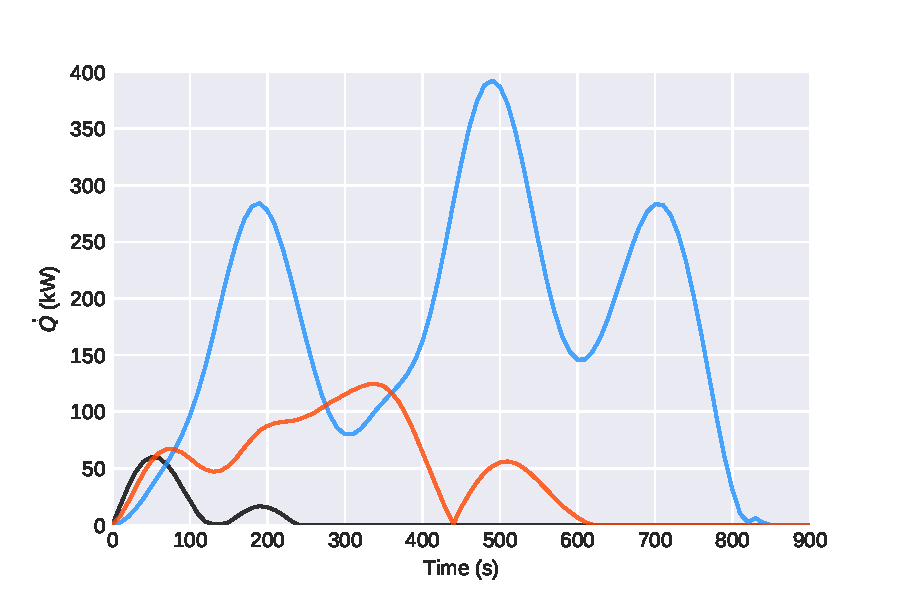
\includegraphics[width=\textwidth,keepaspectratio]{figures/gp_nn_training_smooth.pdf}
      \caption{ $b=60$ sec.}
      \label{fig:gp_nn_training_smooth}
  \end{subfigure}
  \begin{subfigure}[t]{.45\textwidth}
      \centering
      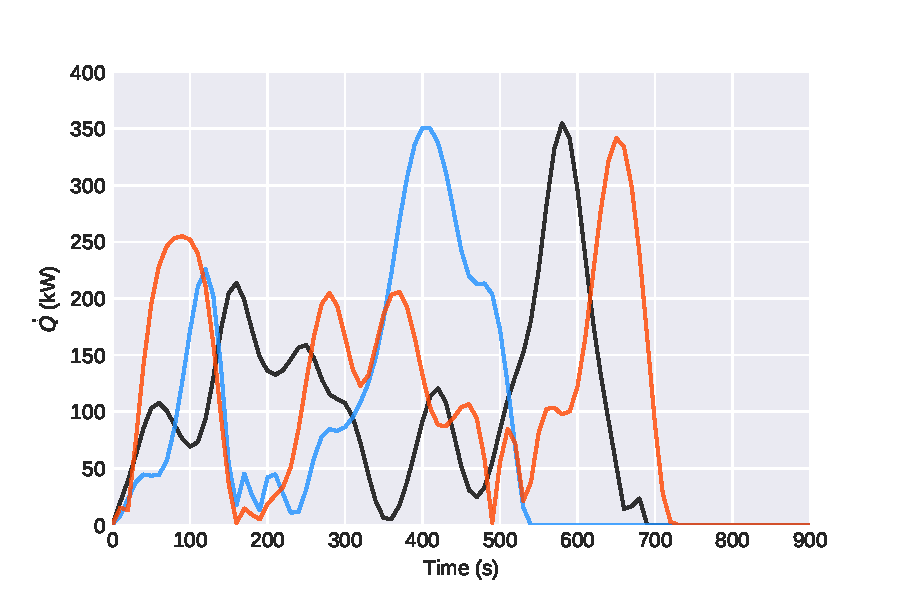
\includegraphics[width=\textwidth ,keepaspectratio]{figures/gp_nn_training_wiggly.pdf}
      \caption{ $b=30$ sec.}
      \label{fig:gp_nn_training_wiggly}
  \end{subfigure}
  \caption{Example draws from the Gaussian processes used to generate the random HRR curves in the neural network training set. \protect\ref{fig:gp_nn_training_smooth} shows that the drawn functions are smoother when the bandwidth is set to 60 seconds compared to those shown in \protect\ref{fig:gp_nn_training_wiggly} using a bandwidth of 30 seconds. The emulators train on functions drawn from both distributions. Note that the HRR curves also have a varying duration so that the emulators can learn to produce the results from FDS simulations with different simulation durations.} 
  \label{fig:gp_nn_training}
\end{figure}







\begin{figure}[htb] \centering
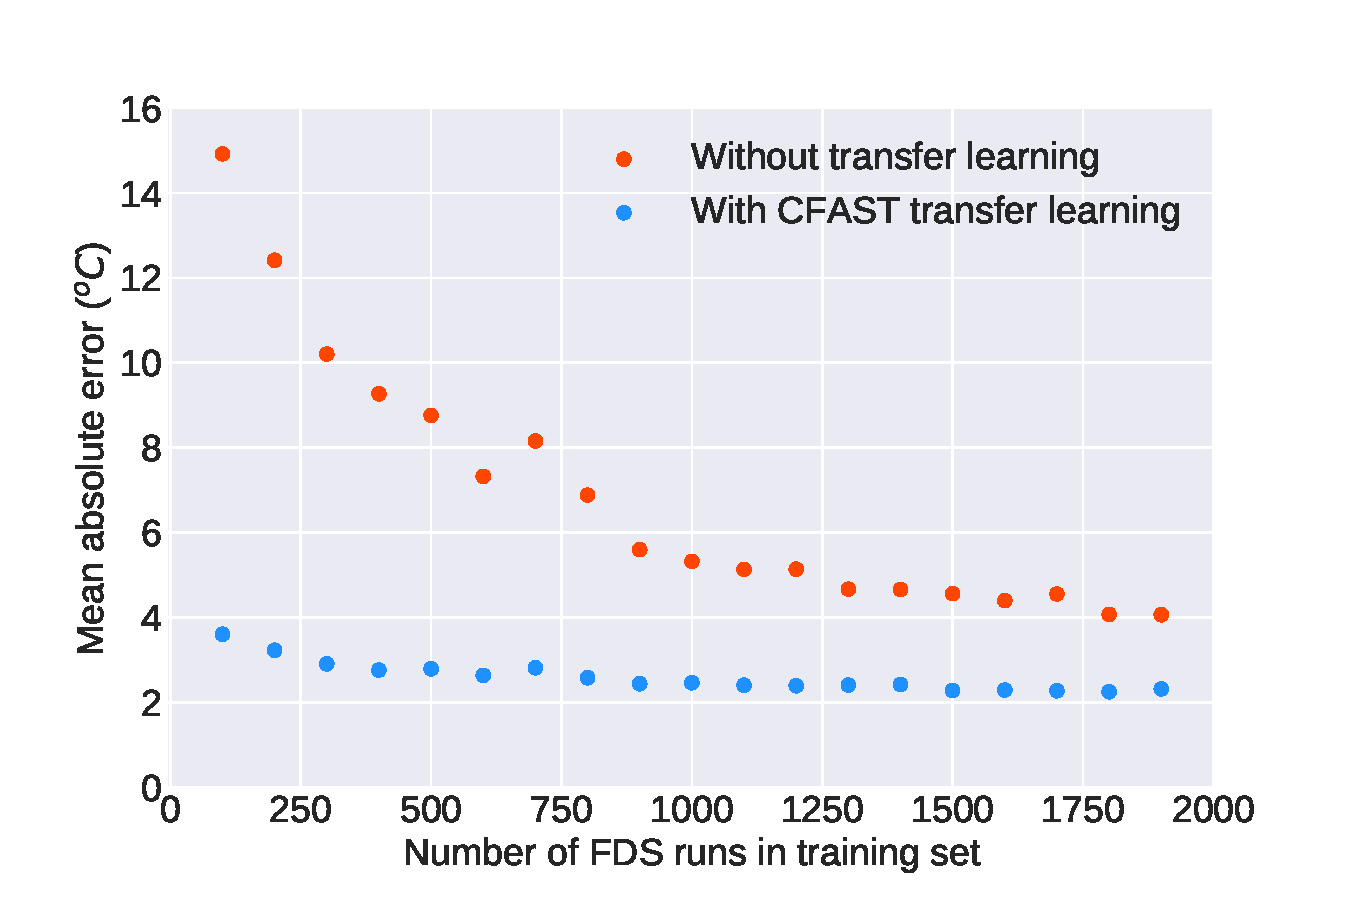
\includegraphics[width=.75\textwidth]{./figures/transfer_learning_effect.pdf}
\caption{A plot demonstrating the effect of transfer learning for one thermocouple response. When the neural network is first trained on 20,000 predictions of the upper gas layer from CFAST, a simplified two zone model, it is able to learn to emulate FDS results with a far smaller training set. }
\label{fig:transfer_learning}
\end{figure}


\begin{figure}[htbp]
  \centering
  \begin{subfigure}[t]{.45\textwidth}
      \centering
      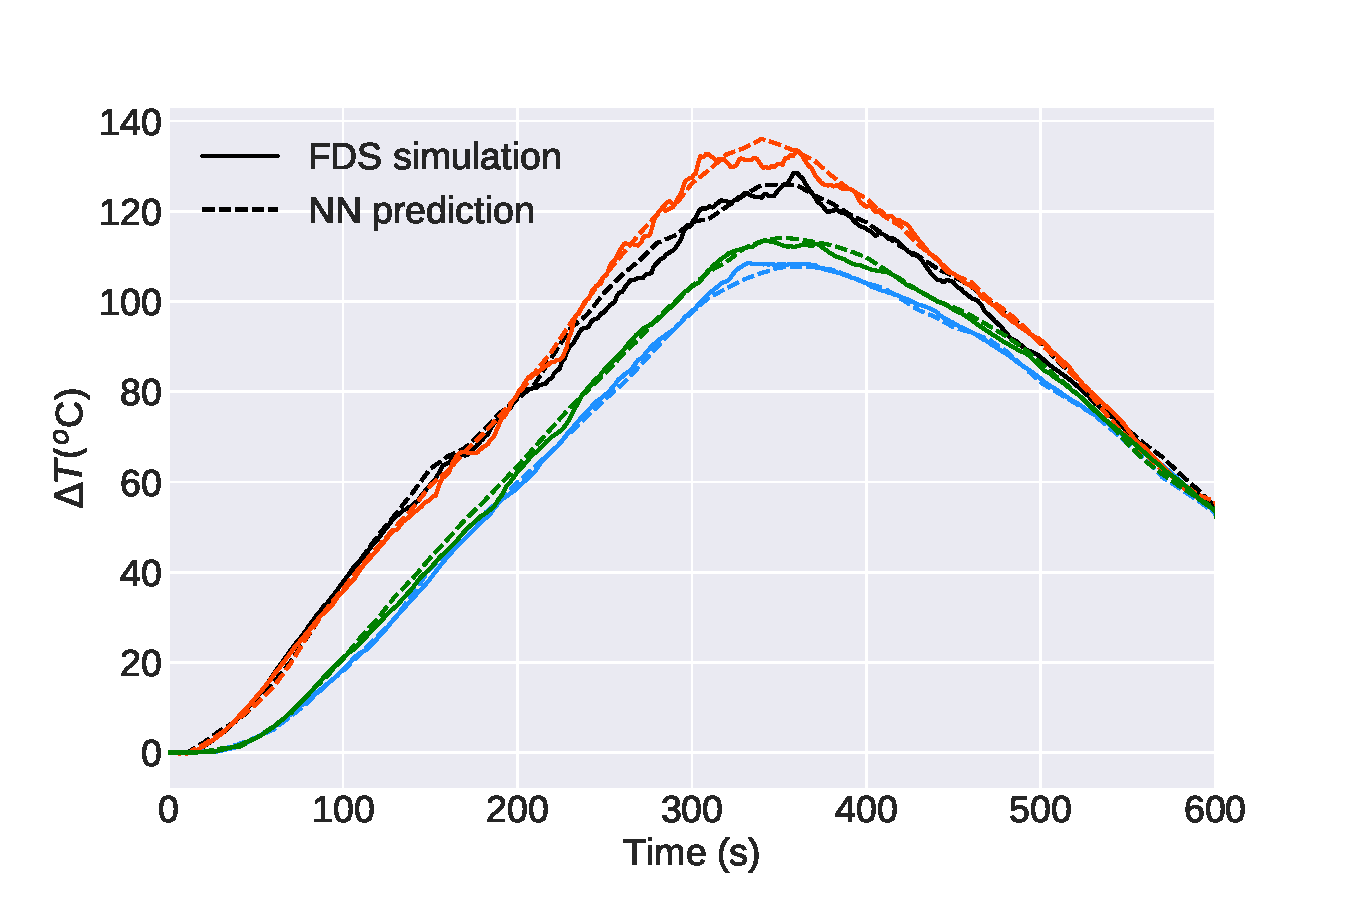
\includegraphics[width=\textwidth,keepaspectratio]{figures/forward_NN_examples.pdf}
      \caption{Example thermocouple responses simulated \\ in FDS compared to the deep learning emulators }
      \label{fig:forward_NN_examples}
  \end{subfigure}
  \begin{subfigure}[t]{.45\textwidth}
      \centering
      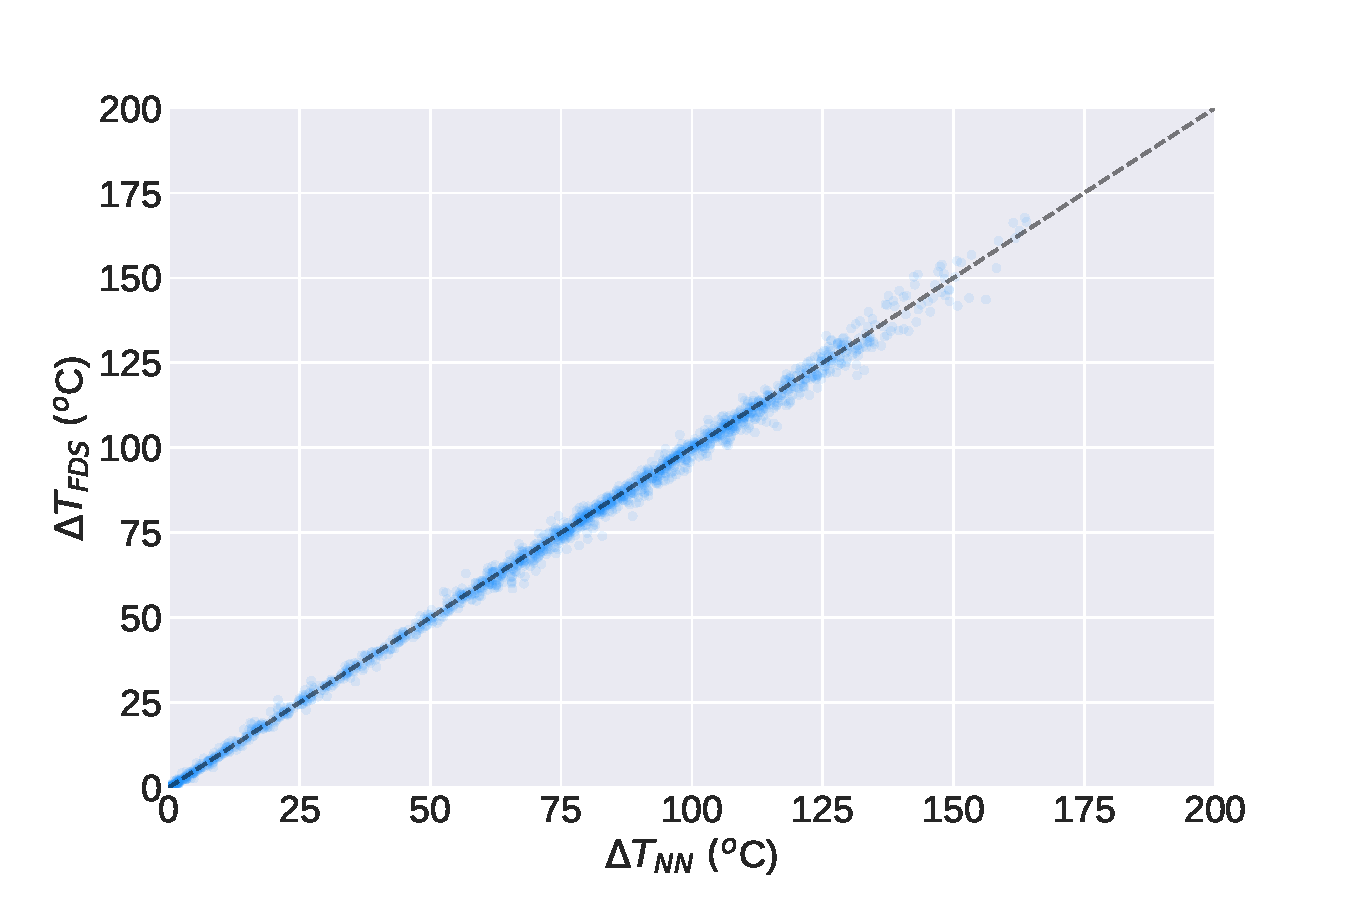
\includegraphics[width=\textwidth ,keepaspectratio]{figures/forward_error_scatter.pdf}
      \caption{Comparison of the FDS simulation results compared to the predictions from the emulators across all times, all three training set tests, and all 17 thermocouples.  }
      \label{fig:forward_error_scatter}
  \end{subfigure}
  \caption{A comparison of the predictions of the deep learning emulators compared to FDS simulations for the experimental fire ramps, which were not in the neural networks training set. \protect\ref{fig:forward_error_scatter} shows that the emulators successfully predict the FDS output with a mean absolute error of <2$^o$ C across all sensors, all times, and all three experiments in Figure \protect\ref{fig:training_ramps}.} 
  \label{fig:forward_error}
\end{figure}

\begin{figure}[htb] \centering
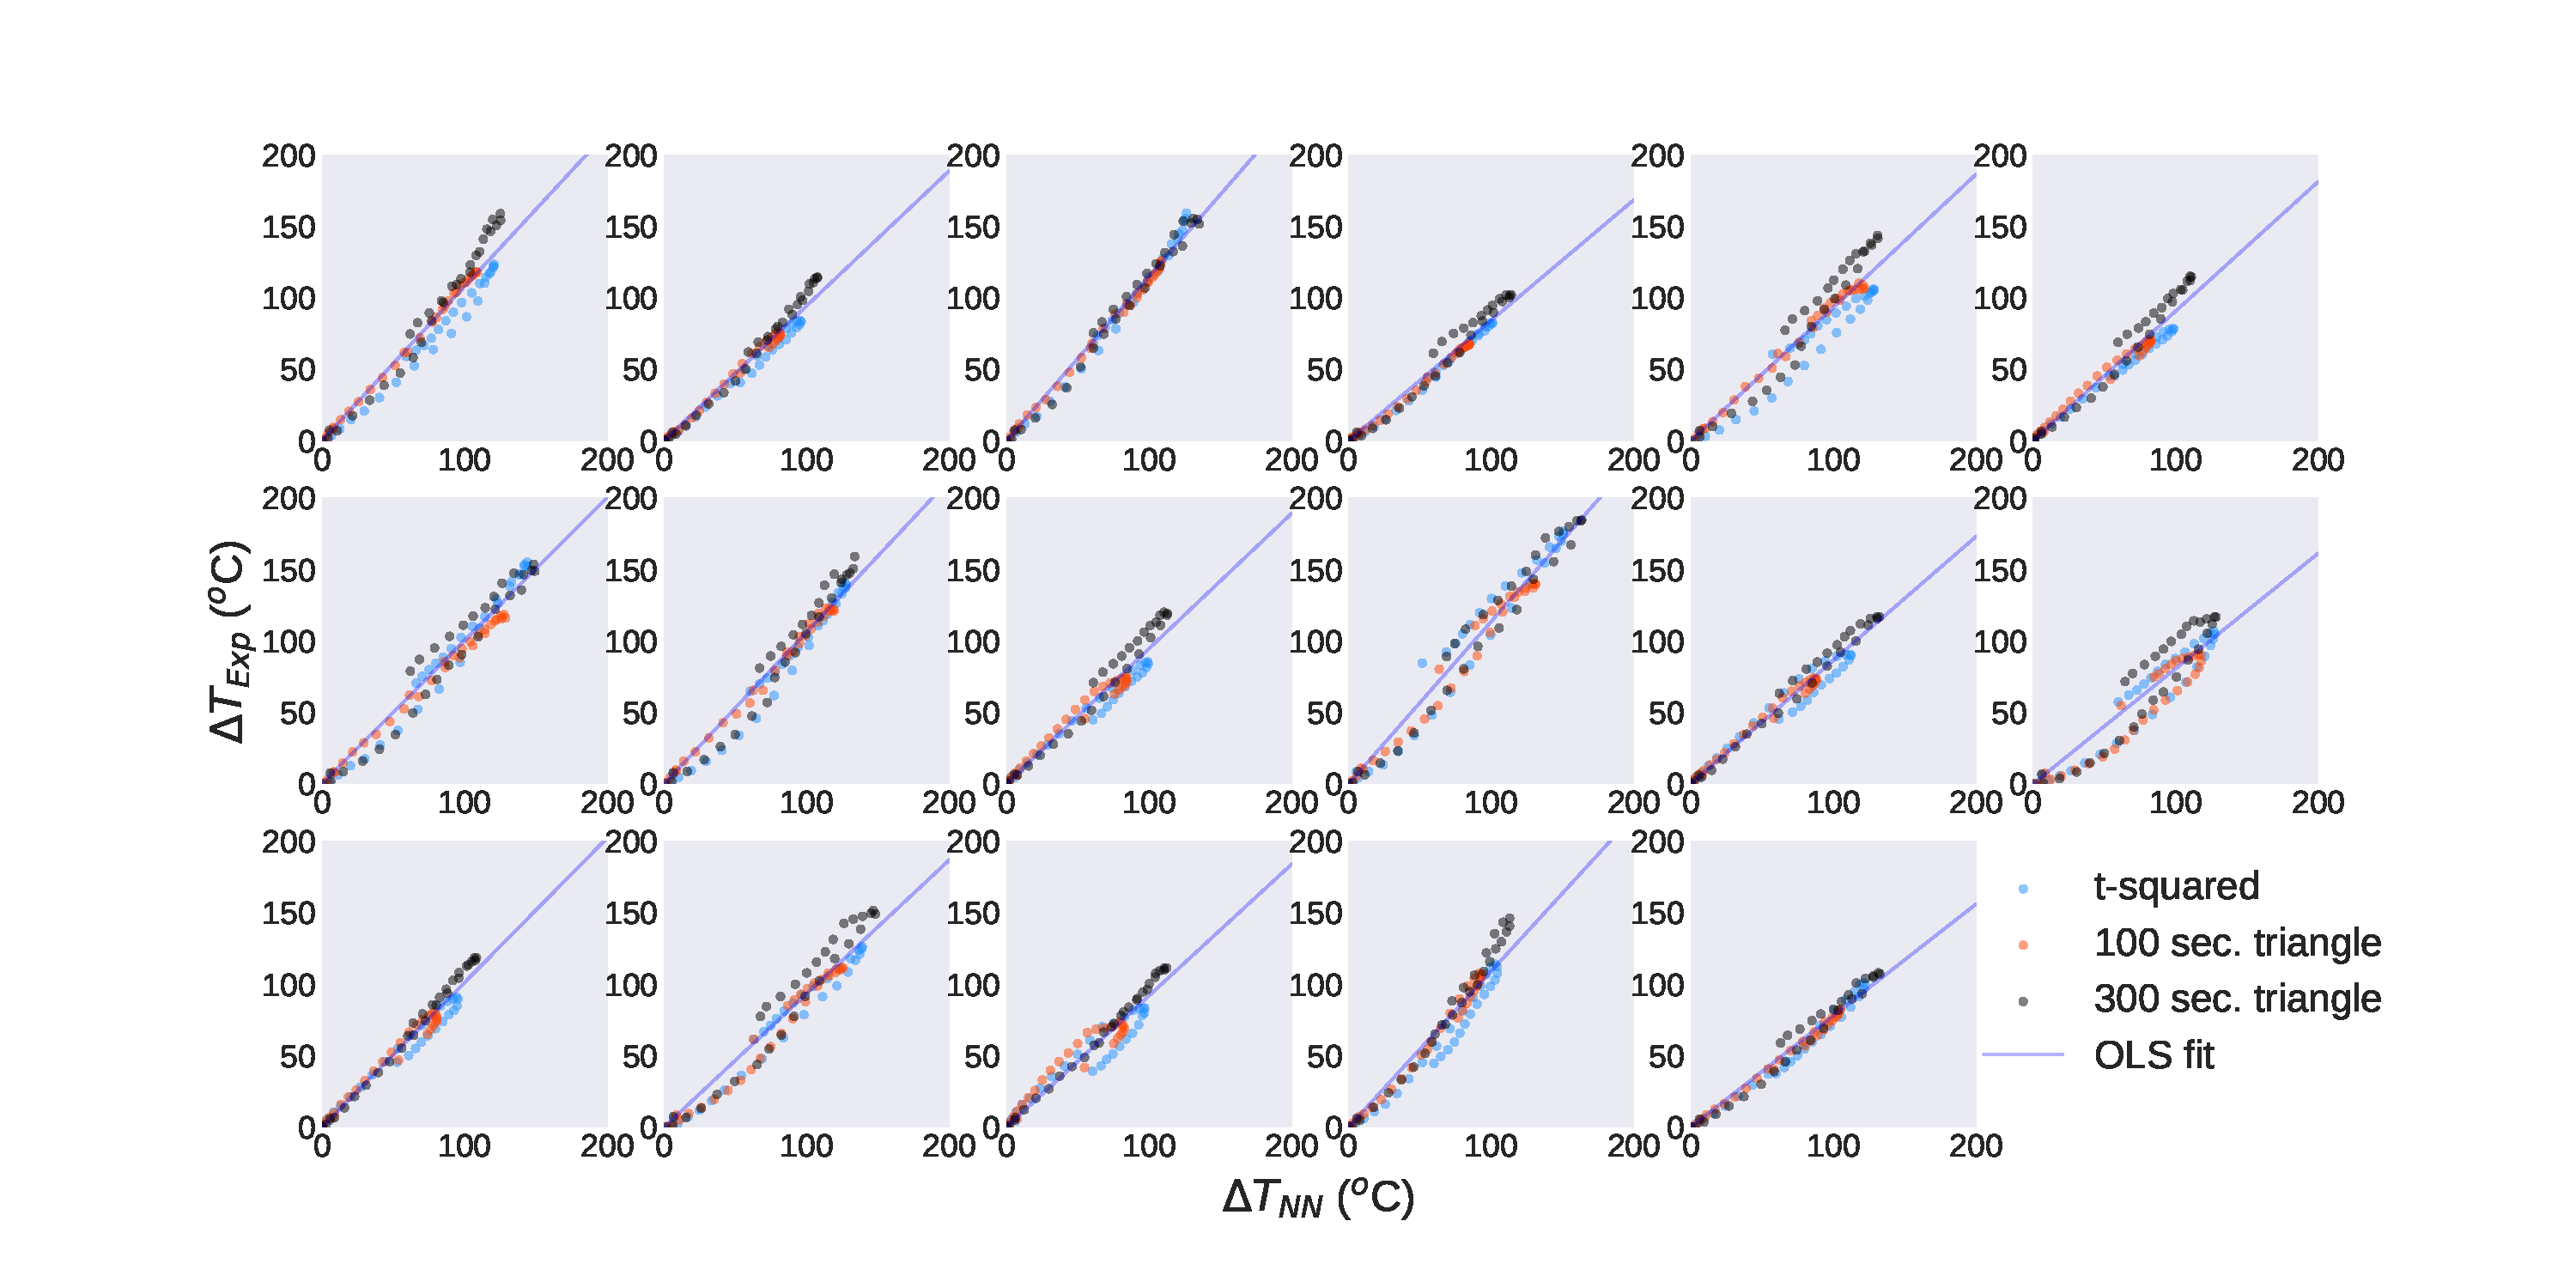
\includegraphics[width=.9\textwidth]{figures/fds_vs_reality.pdf}
\caption{}
\label{fig:fds_vs_reality}
\end{figure}

\begin{figure}[htbp]
  \centering
  \begin{subfigure}[t]{.45\textwidth}
      \centering
      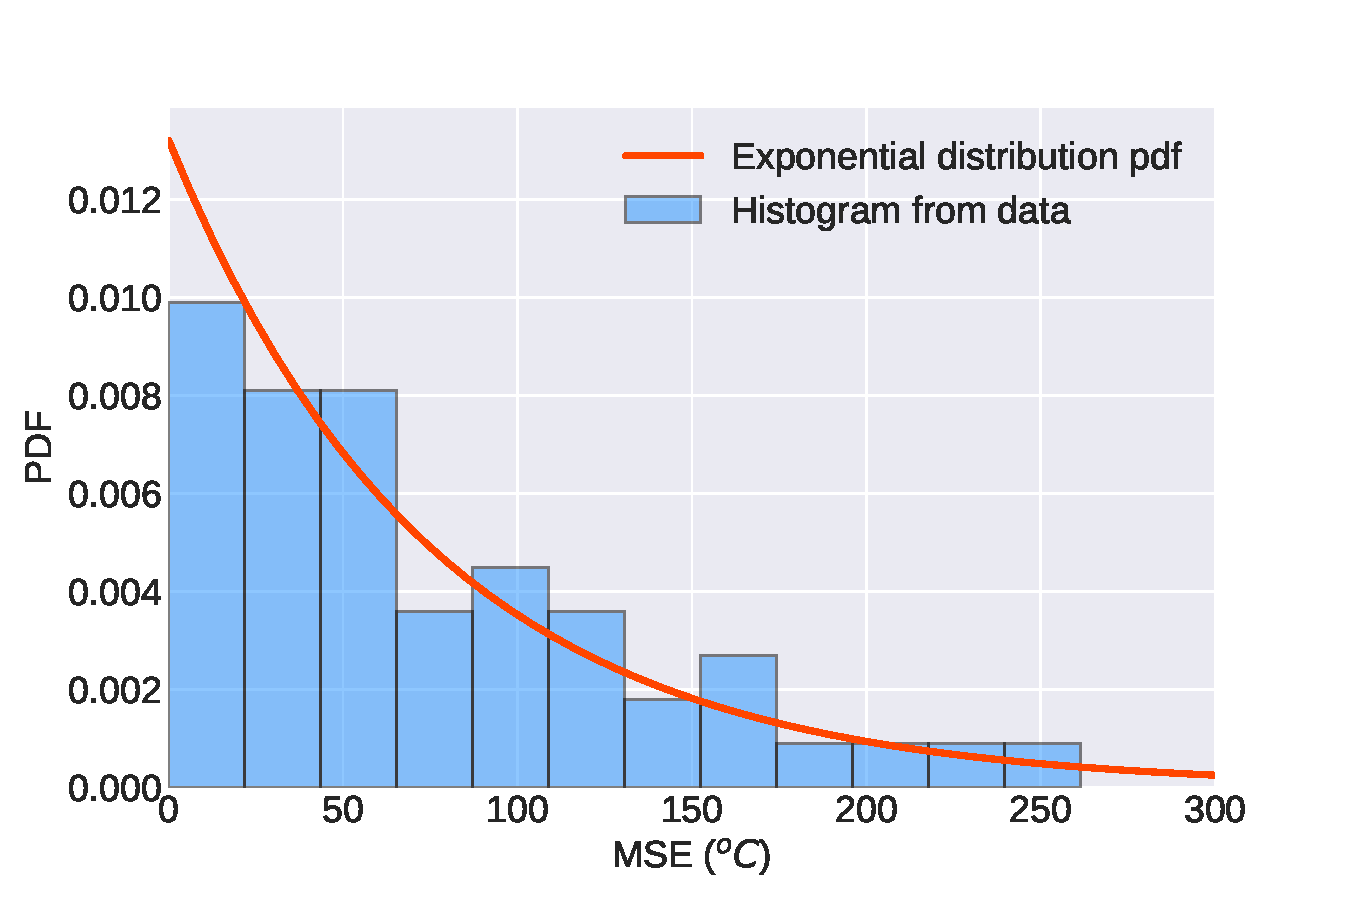
\includegraphics[width=\textwidth,keepaspectratio]{figures/misfit_pdf.pdf}
      \caption{}
      \label{fig:misfit_pdf}
  \end{subfigure}
  \begin{subfigure}[t]{.45\textwidth}
      \centering
      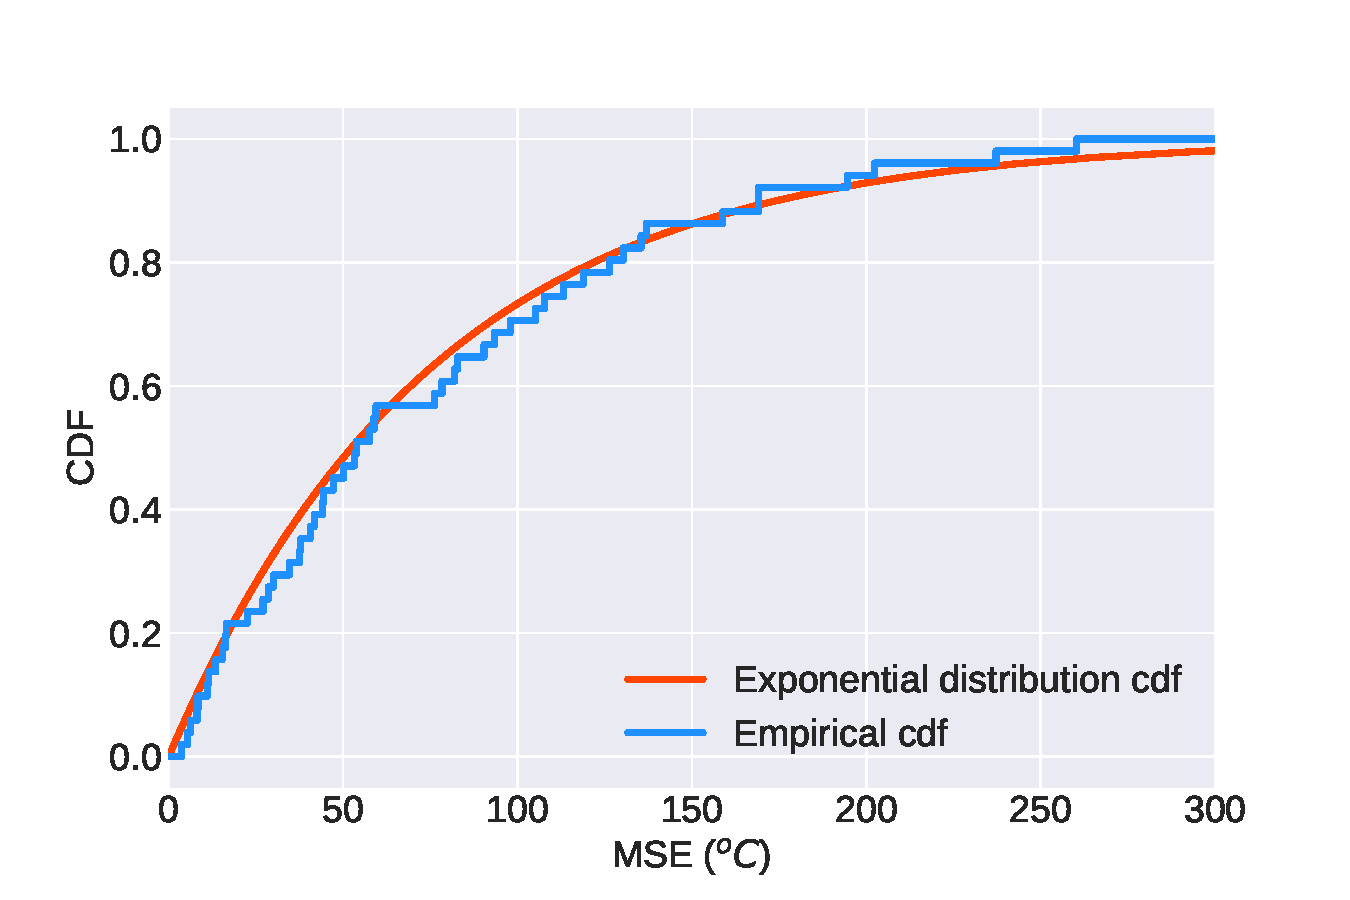
\includegraphics[width=\textwidth ,keepaspectratio]{figures/misfit_cdf.pdf}
      \caption{}
      \label{fig:misfit_cdf}
  \end{subfigure}
  \caption{} 
  \label{fig:misfit_distribution}
\end{figure}

\begin{figure}[htbp]
  \centering
  \begin{subfigure}[t]{.45\textwidth}
      \centering
      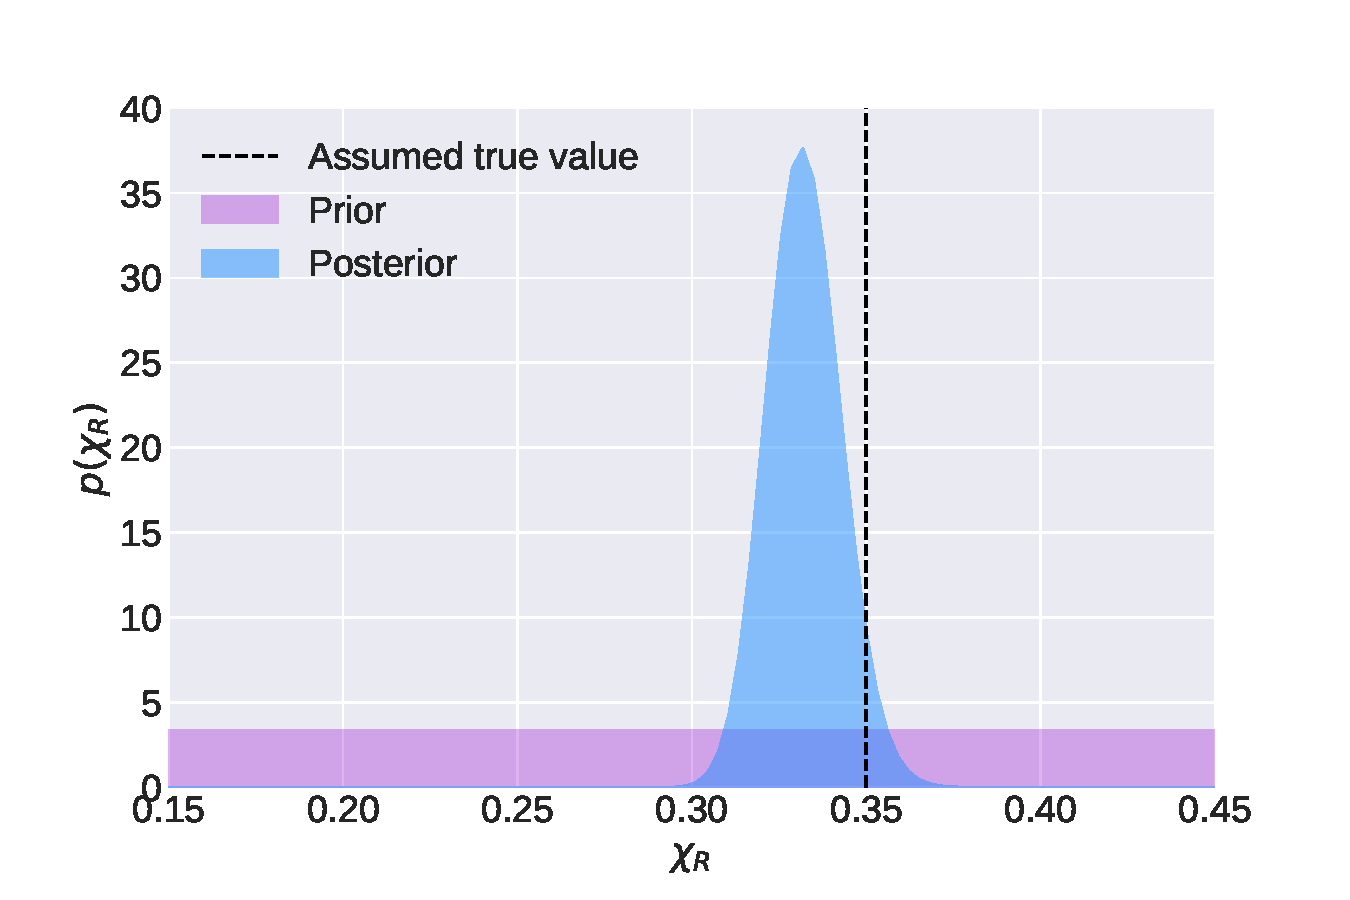
\includegraphics[width=\textwidth,keepaspectratio]{figures/bayes_distributions.pdf}
      \caption{}
      \label{fig:bayes_distributions}
  \end{subfigure}
  \begin{subfigure}[t]{.45\textwidth}
      \centering
      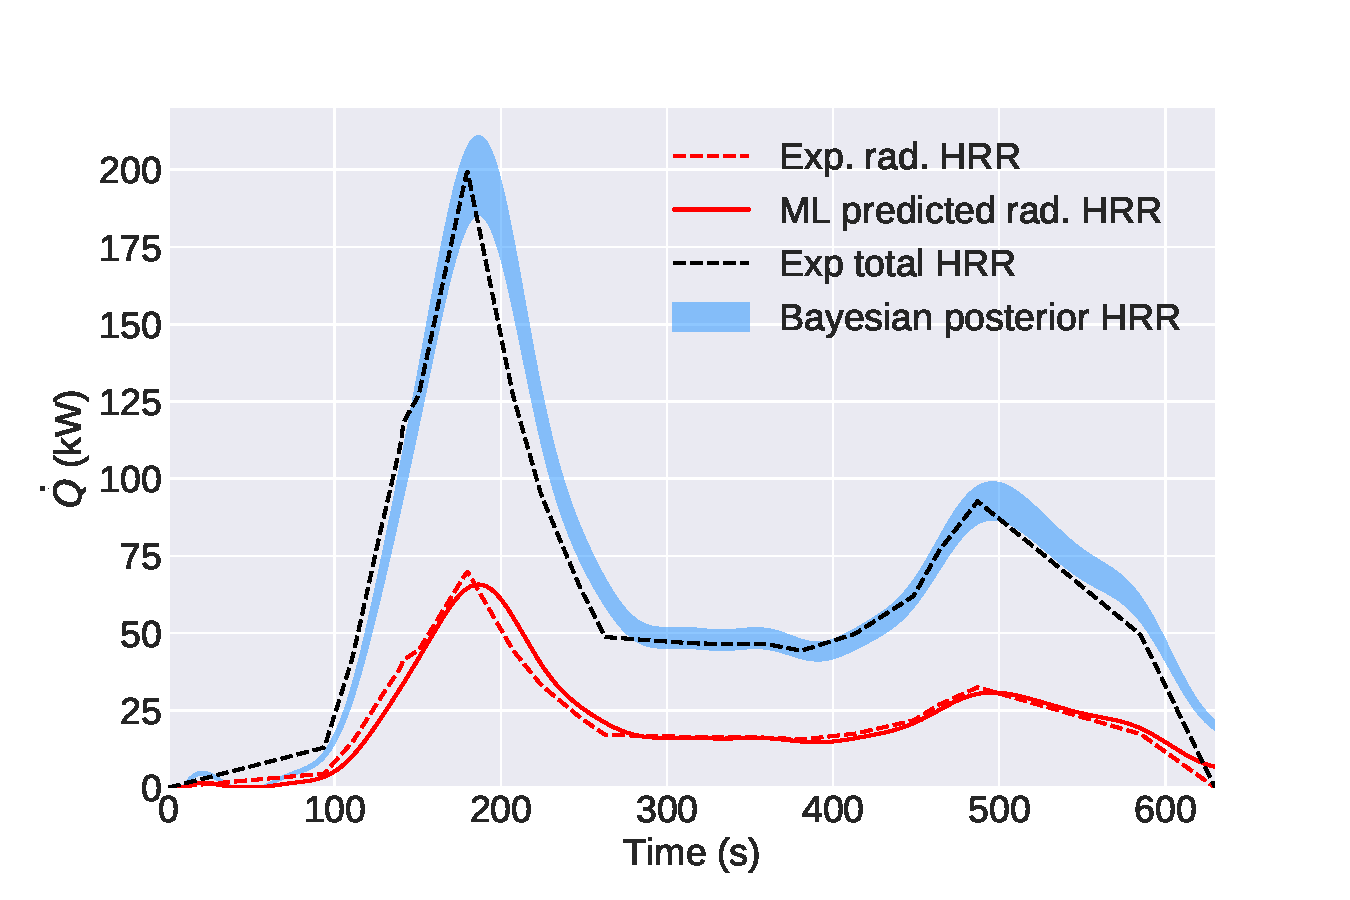
\includegraphics[width=\textwidth ,keepaspectratio]{figures/bayes_burner_result.pdf}
      \caption{}
      \label{fig:burner_result}
  \end{subfigure}
  \caption{} 
  \label{fig:bayes_result}
\end{figure}

\clearpage
\subsubsection{Backward FDS emulators}

\begin{figure}[htbp]
  \centering
  \begin{subfigure}[t]{.45\textwidth}
      \centering
      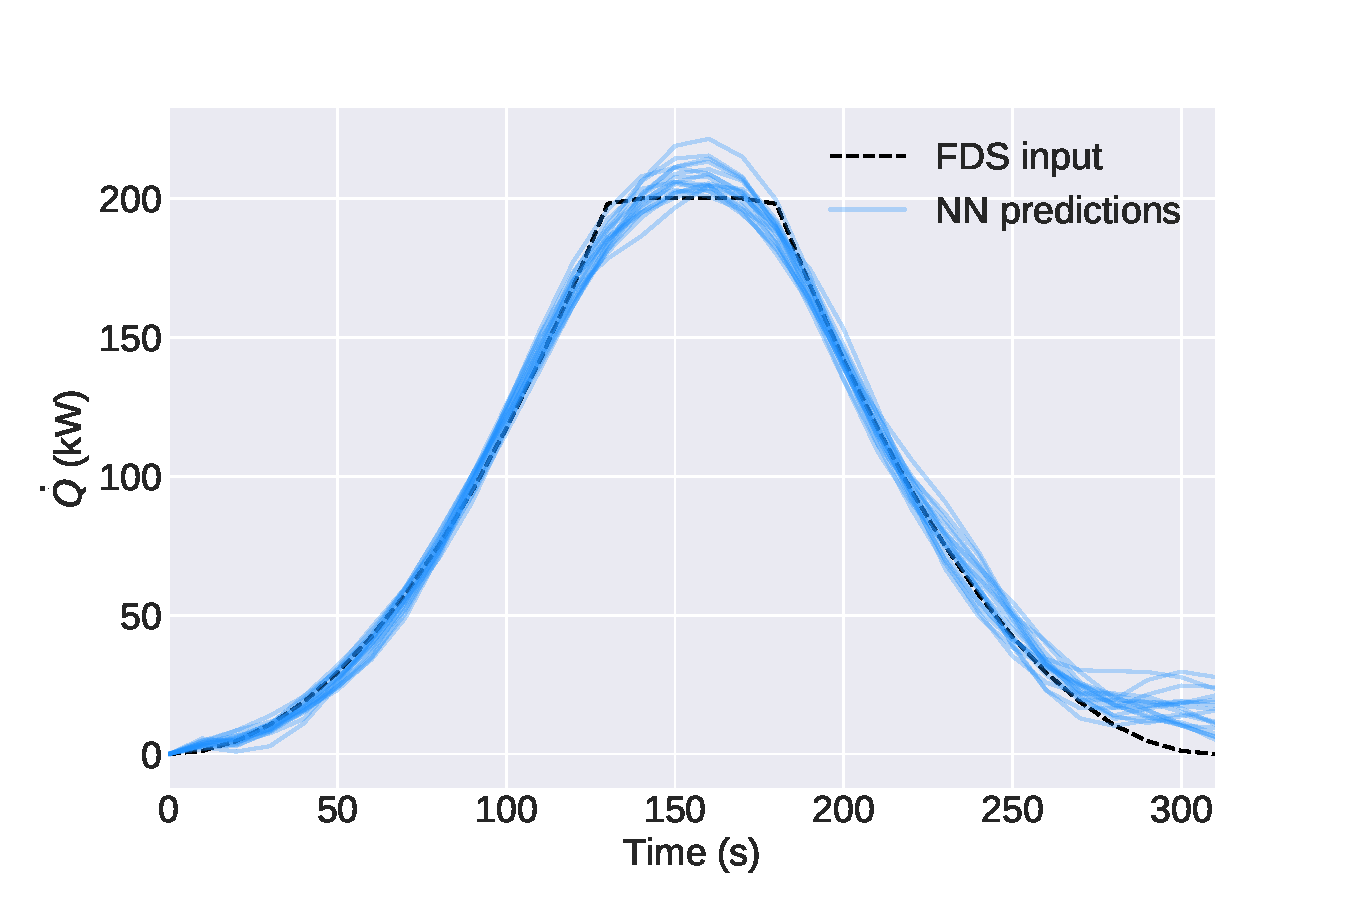
\includegraphics[width=\textwidth,keepaspectratio]{figures/backward_NN_examples.pdf}
      \caption{}
      \label{fig:backward_NN_examples}
  \end{subfigure}
  \begin{subfigure}[t]{.45\textwidth}
      \centering
      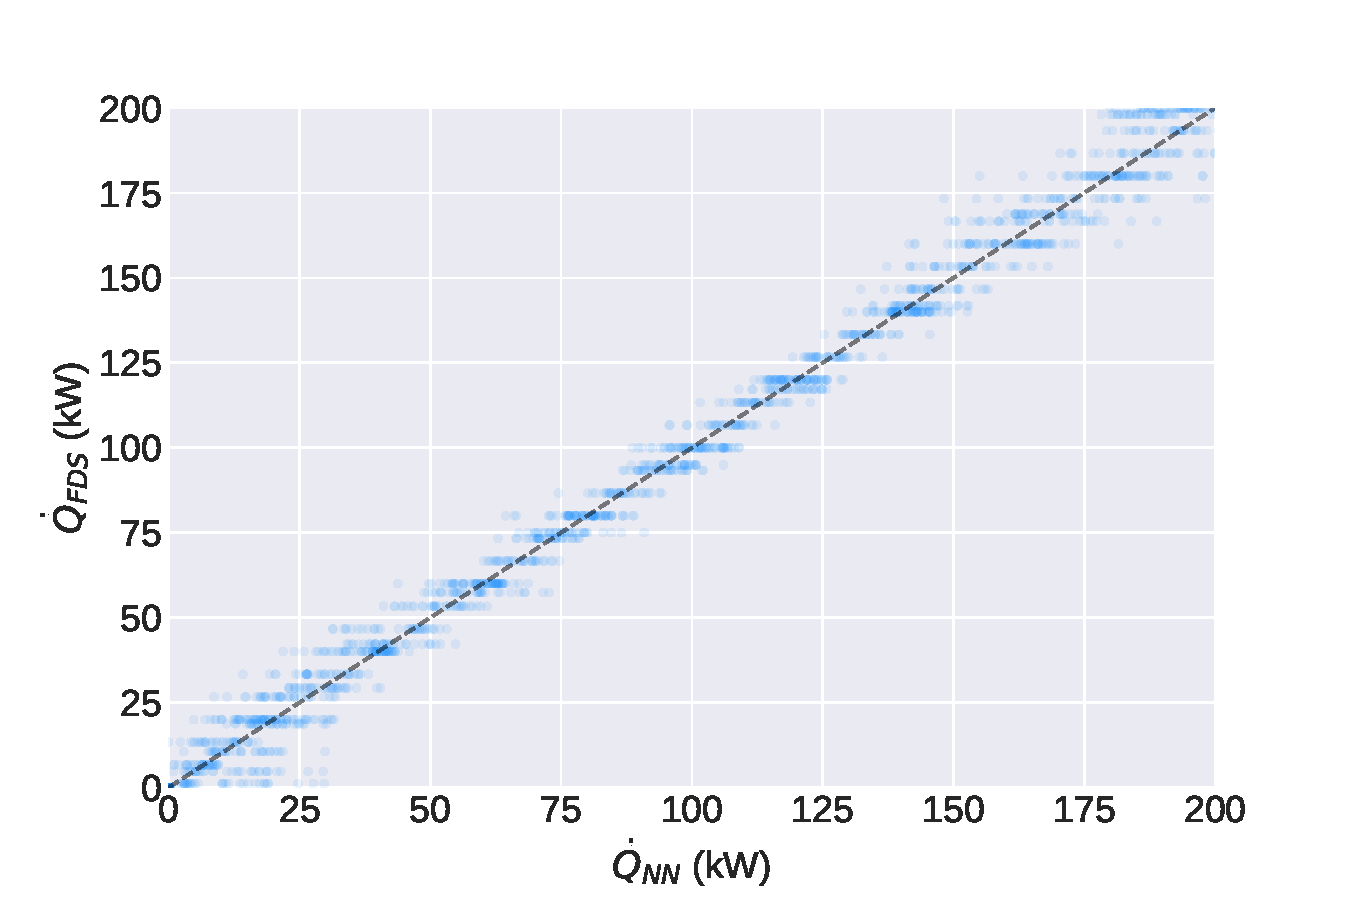
\includegraphics[width=\textwidth ,keepaspectratio]{figures/backward_error_scatter.pdf}
      \caption{}
      \label{fig:backward_error_scatter}
  \end{subfigure}
  \caption{} 
  \label{fig:backward_examples}
\end{figure}


\begin{figure}[htb] \centering
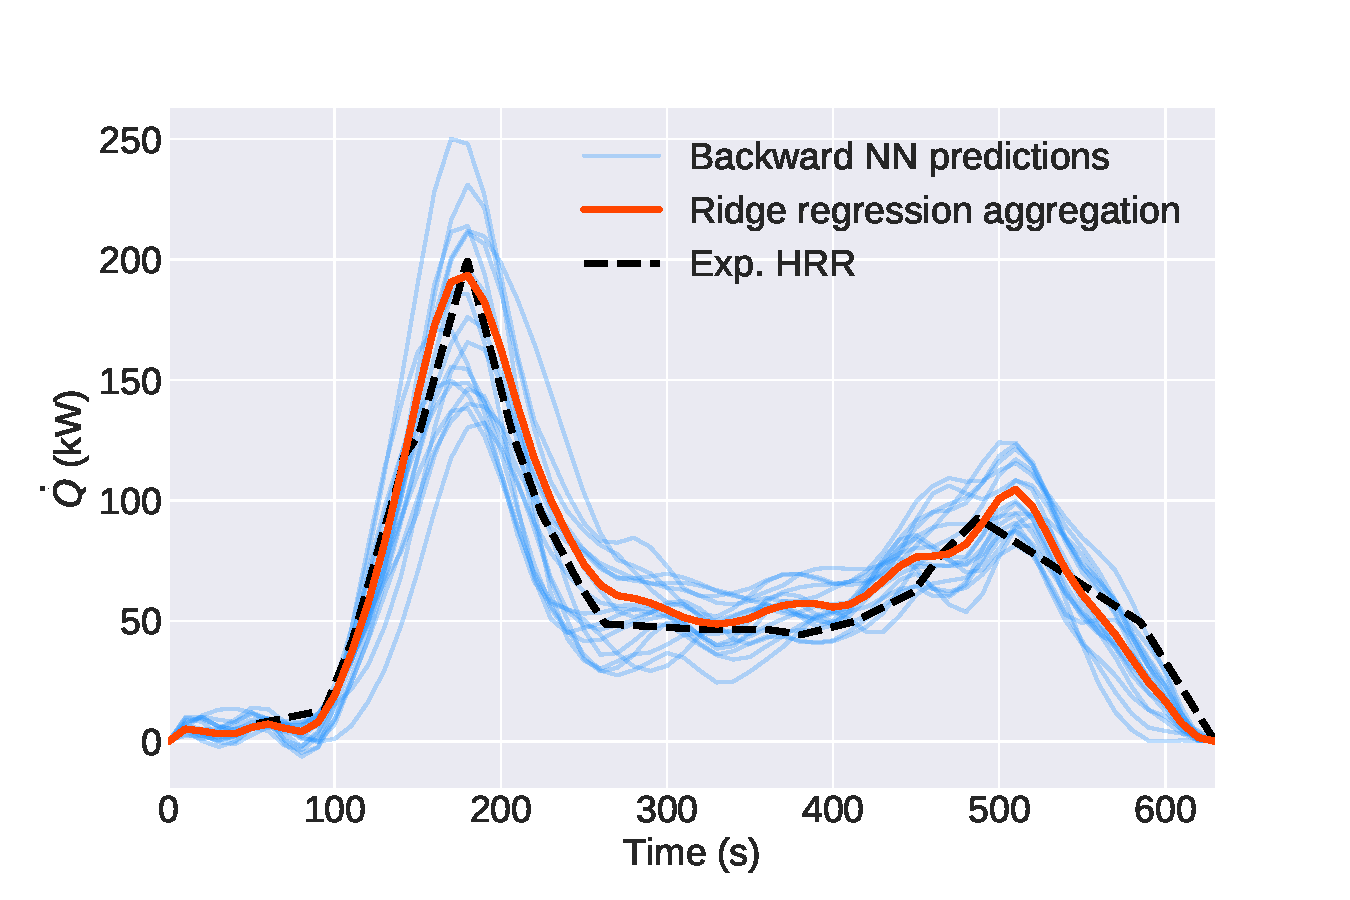
\includegraphics[width=.75\textwidth]{figures/backward_ridge_aggregation.pdf}
\caption{}
\label{fig:backward_ridge_aggregation}
\end{figure}


\begin{figure}[htbp]
  \centering
  \begin{subfigure}[t]{.45\textwidth}
      \centering
      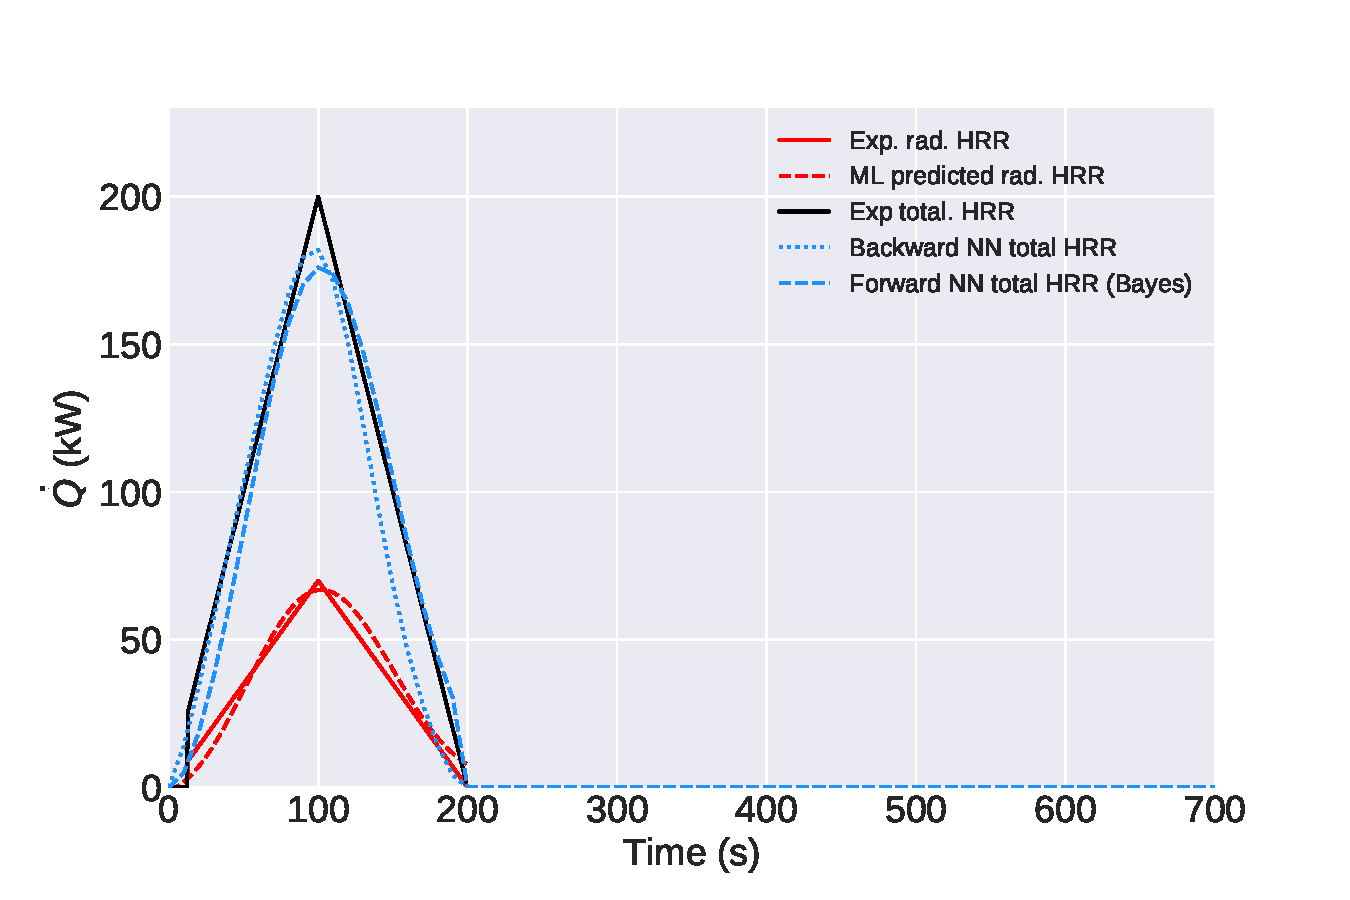
\includegraphics[width=\textwidth,keepaspectratio]{figures/100s_triangle_final.pdf}
      \caption{}
      \label{fig:final_result_100s_triangle}
  \end{subfigure}
  \begin{subfigure}[t]{.45\textwidth}
      \centering
      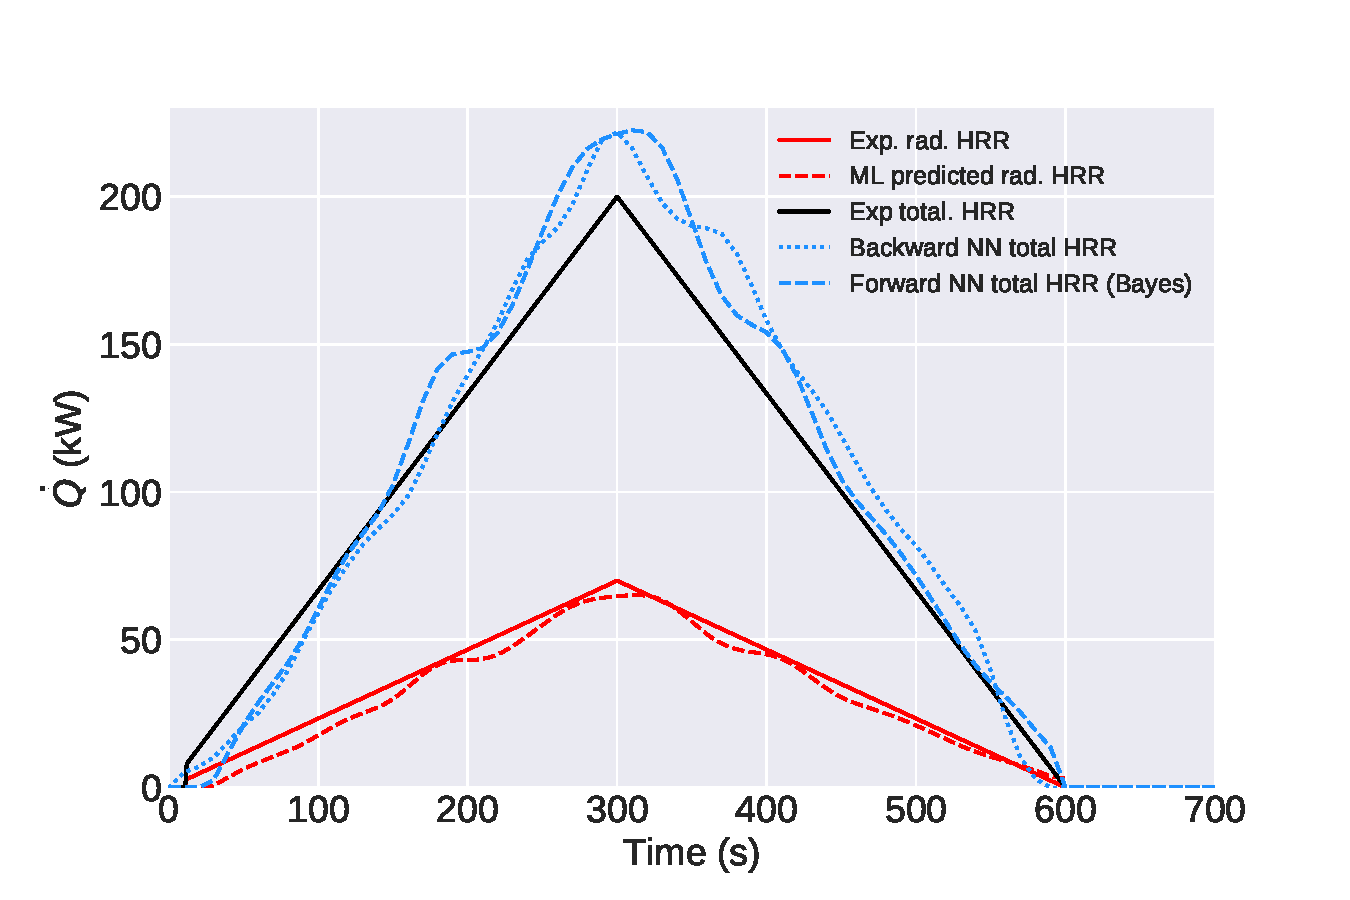
\includegraphics[width=\textwidth ,keepaspectratio]{figures/300s_triangle_final.pdf}
      \caption{}
      \label{fig:final_result_300s_triangle}
  \end{subfigure}
   \begin{subfigure}[t]{.45\textwidth}
      \centering
      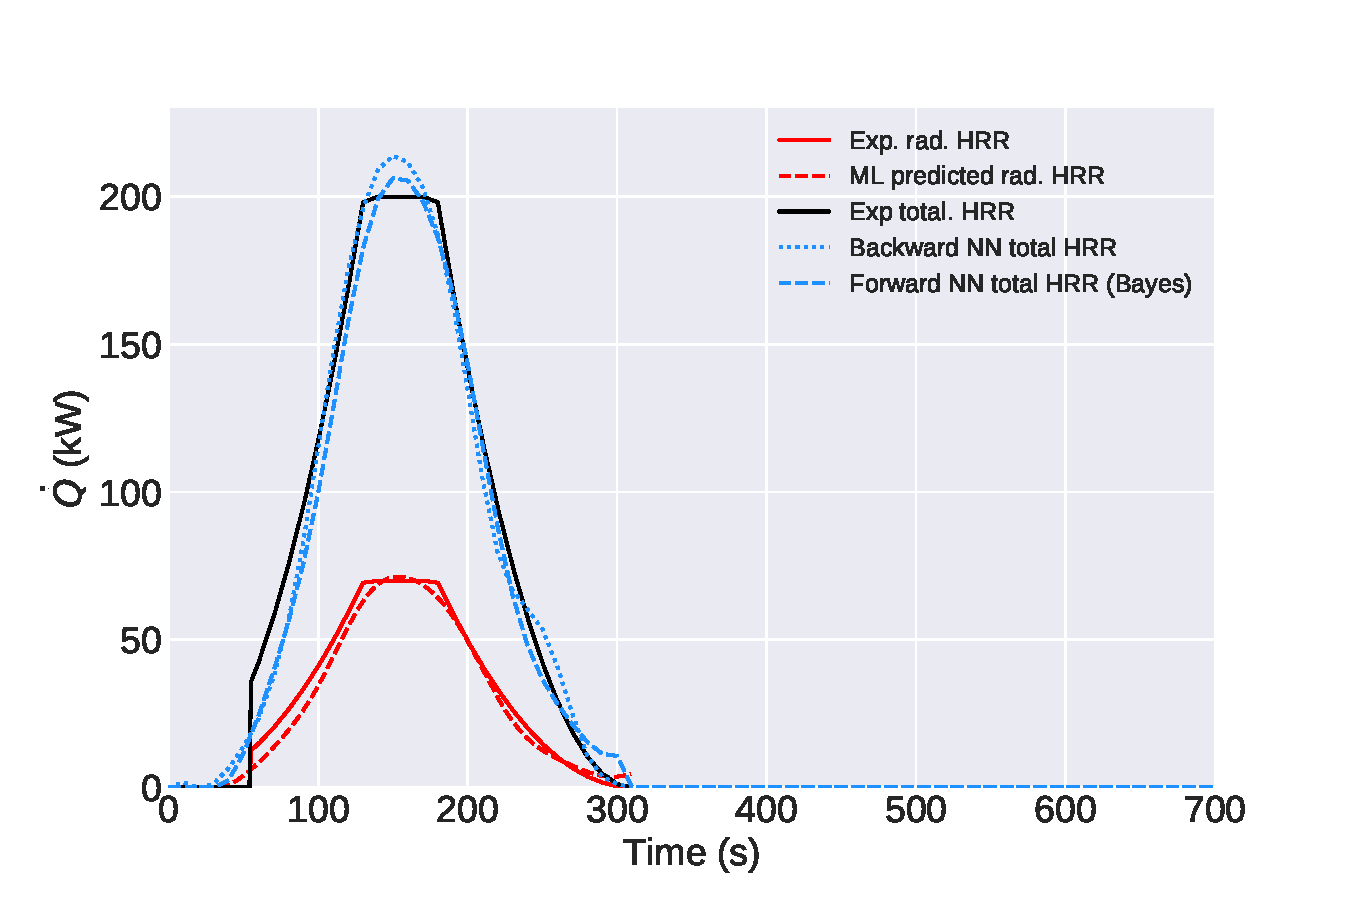
\includegraphics[width=\textwidth ,keepaspectratio]{figures/t_squared_final.pdf}
      \caption{}
      \label{fig:final_result_t_squared}
  \end{subfigure}
    \begin{subfigure}[t]{.45\textwidth}
      \centering
      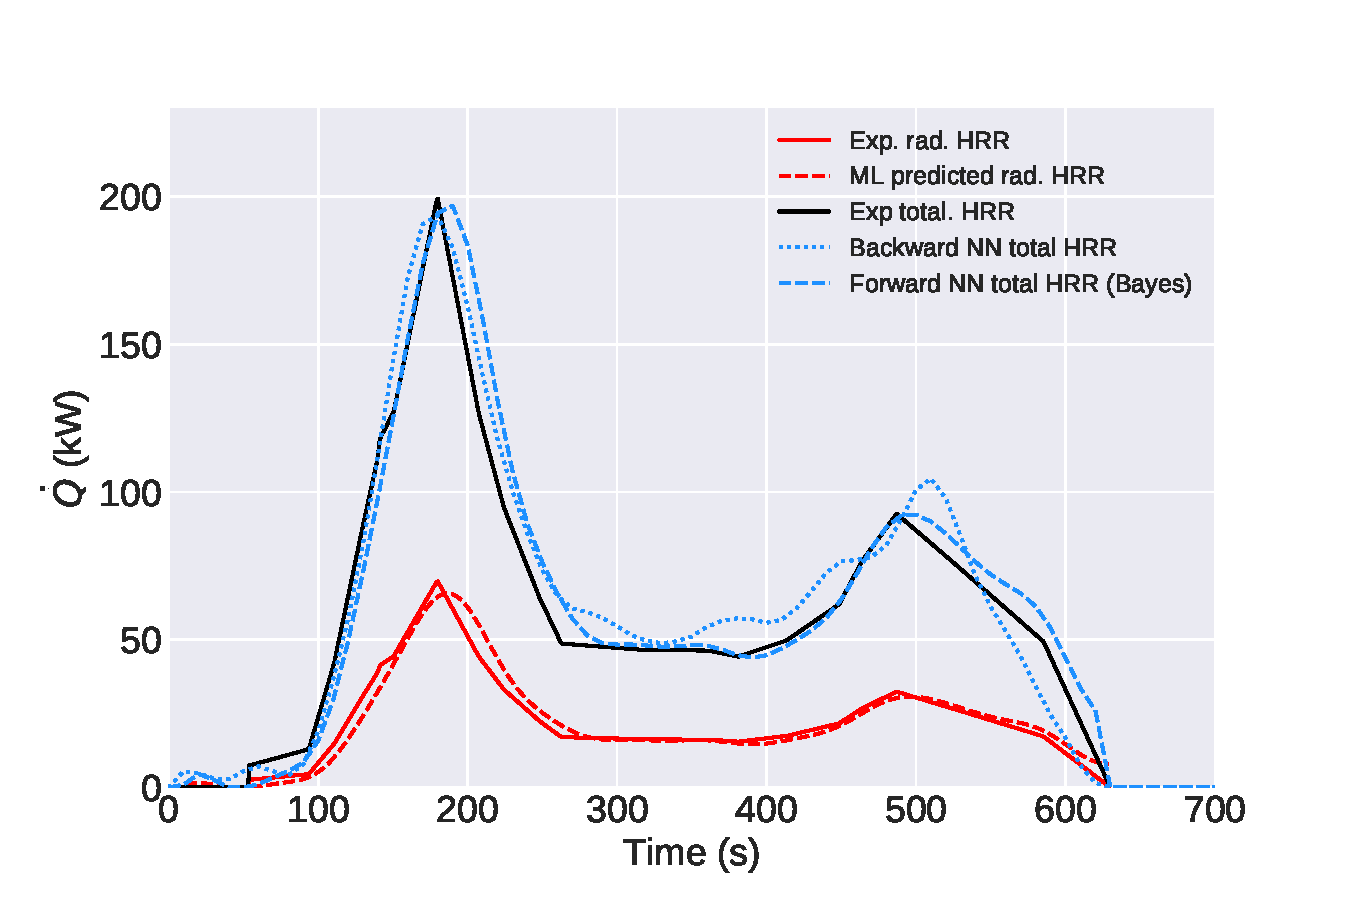
\includegraphics[width=\textwidth ,keepaspectratio]{figures/weird_curve_final.pdf}
      \caption{}
      \label{fig:final_result_weird_curve}
  \end{subfigure}
  \caption{} 
  \label{fig:final_burner_results}
\end{figure}


\begin{figure}[htbp]
  \centering
  \begin{subfigure}[t]{.45\textwidth}
      \centering
      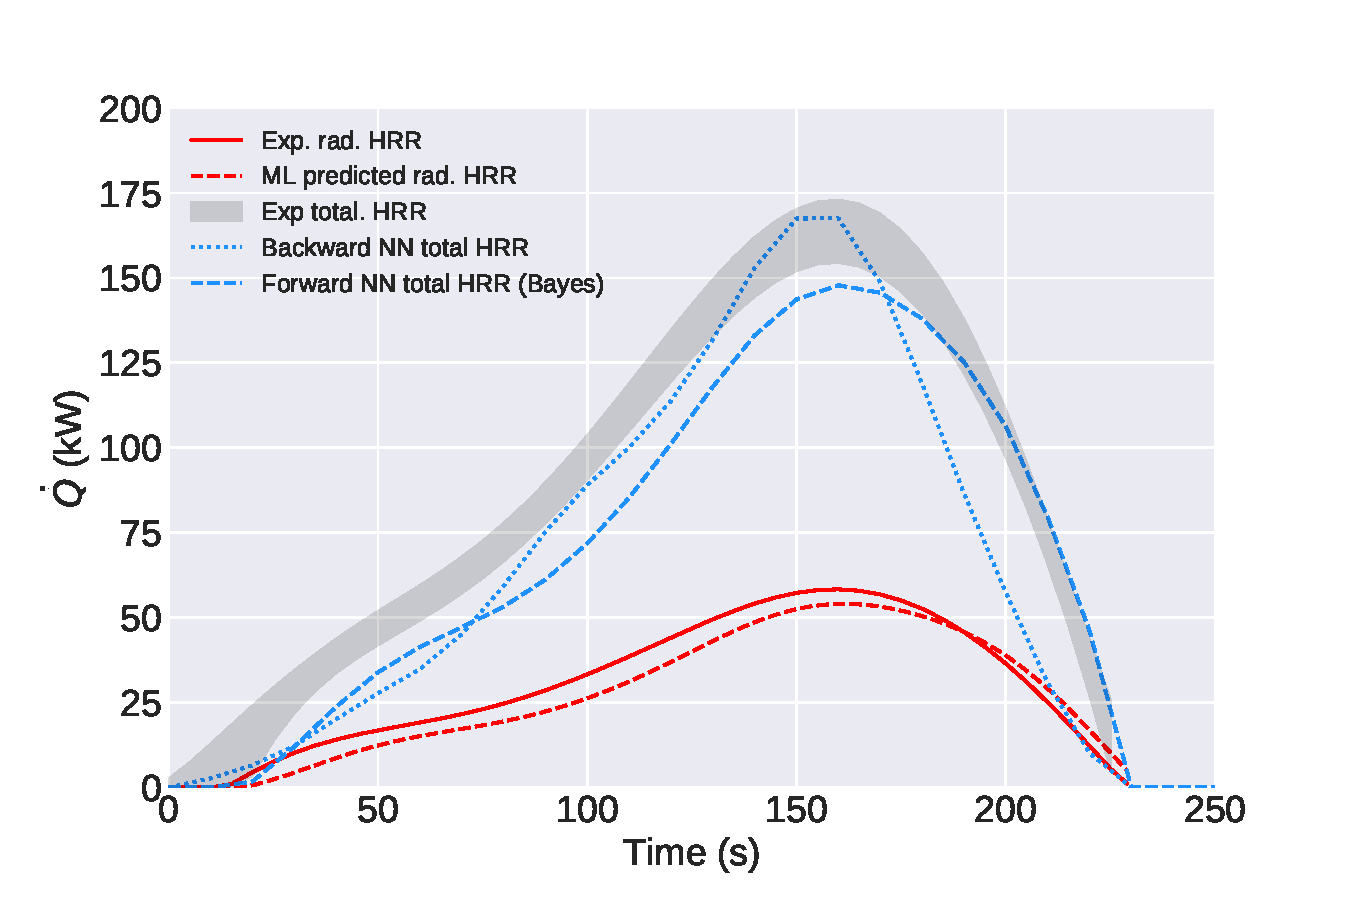
\includegraphics[width=\textwidth,keepaspectratio]{figures/nhex_12in_1_final.pdf}
      \caption{}
      \label{fig:nhex_12in_1}
  \end{subfigure}
  \begin{subfigure}[t]{.45\textwidth}
      \centering
      \includegraphics[width=\textwidth ,keepaspectratio]{figures/nhex_12in_2_final.pdf}
      \caption{}
      \label{fig:nhex_12in_2}
  \end{subfigure}
  \caption{} 
  \label{fig:nhex_fires}
\end{figure}


\begin{figure}[htbp]
  \centering
  \begin{subfigure}[t]{.45\textwidth}
      \centering
      \includegraphics[width=\textwidth,keepaspectratio]{figures/meth_22in_1_final.pdf}
      \caption{}
      \label{fig:meth_22in_1}
  \end{subfigure}
  \begin{subfigure}[t]{.45\textwidth}
      \centering
      \includegraphics[width=\textwidth ,keepaspectratio]{figures/meth_22in_2_final.pdf}
      \caption{}
      \label{fig:meth_22in_2}
  \end{subfigure}
  \caption{} 
  \label{fig:meth_fires}
\end{figure}
\clearpage


\bibliographystyle{unsrtnat}
\bibliography{./references.bib}
\end{document}
